
\documentclass{article} % For LaTeX2e
\usepackage{iclr2026_conference,times}

% Optional math commands from https://github.com/goodfeli/dlbook_notation.
\input{math_commands.tex}

\usepackage{hyperref}
\usepackage{url}

\usepackage{tcolorbox}
\usepackage{mdframed}
\usepackage{enumitem}
% \usepackage{graphicx}
\usepackage{booktabs}
\usepackage{multirow}

\usepackage{algorithm}
\usepackage{algorithmic}
\usepackage{subcaption}
\usepackage{amsmath}
% \usepackage{amssymb}
\usepackage{pifont}
\usepackage{tabularx}
% \usepackage{float}
% \usepackage{wrapfig}
% \usepackage{subfig}
\usepackage{colortbl}
\usepackage{enumitem}
\usepackage{fancyhdr}
% \usepackage{bbding}
% \usepackage{lipsum} % For filler text
\usepackage{mdframed}
\usepackage{amsmath,amssymb,amsthm}
% \usepackage[most]{tcolorbox}

\usepackage{times}
\usepackage{latexsym}
\usepackage{titletoc}

\usepackage{inconsolata}
\usepackage{makecell}
\usepackage[utf8]{inputenc}
\usepackage[T1]{fontenc}

\usepackage{wrapfig}

\definecolor{lightpink}{RGB}{255, 230, 230} % #FFCCCC
\definecolor{darkred}{RGB}{185, 38, 74}    
\definecolor{darkgreen}{RGB}{0,100,0}
\newmdenv[
  backgroundcolor=gray!5,
  skipabove=1em,
  skipbelow=0em,
  leftline=true,
  topline=false,
  bottomline=false,
  rightline=false,
  linecolor=gray!70,
  linewidth=1.5pt
]{githubquote}


% \DeclareCaptionStyle{ruled}{labelfont=normalfont,labelsep=colon,strut=off} % DO NOT CHANGE THIS
% \lstset{%
% 	basicstyle={\footnotesize\ttfamily},% footnotesize acceptable for monospace
% 	numbers=left,numberstyle=\footnotesize,xleftmargin=2em,% show line numbers, remove this entire line if you don't want the numbers.
% 	aboveskip=0pt,belowskip=0pt,%
% 	showstringspaces=false,tabsize=2,breaklines=true}
% \floatstyle{ruled}
% \newfloat{listing}{tb}{lst}{}
% \floatname{listing}{Listing}


\newtcolorbox{myboxi}[1][Default Title]{
  % breakable,
  title=#1,
  % colback=white,
  colback=red!5,
  colbacktitle=red!5,
  coltitle=black,
  fonttitle=\bfseries,
  bottomrule=0pt,
  toprule=0pt,
  leftrule=1.5pt,
  rightrule=1.5pt,
  titlerule=0.5pt,
  arc=0pt,
  outer arc=0pt,
  colframe=red!50,
}


\title{Beyond Student: An Asymmetric Network for Neural Network Inheritance}



% Authors must not appear in the submitted version. They should be hidden
% as long as the \iclrfinalcopy macro remains commented out below.
% Non-anonymous submissions will be rejected without review.

\author{Yiyun Zhou~$^{\spadesuit}$\thanks{Equal contribution.} ~~ Jingwei Shi~$^{\heartsuit}$\footnotemark[1] ~~ Mingjing Xu~$^{\clubsuit}$\footnotemark[1] ~~ Zhonghua Jiang~$^{\spadesuit}$ ~~ Jingyuan Chen~$^{\spadesuit}$\thanks{Corresponding author.} \\\\
$^\spadesuit$Zhejiang University ~~ $^{\heartsuit}$Shanghai University of Finance and Economics ~~ $^{\clubsuit}$ Swansea University \\
\texttt{\{yiyunzhou, jiangzhonghua, jingyuanchen\}@zju.edu.cn} ~~ \texttt{shijingwei@stu.sufe.edu.cn} ~~ \\ \texttt{mingjing.xu@swansea.ac.uk} \\\\
Demo Code:~\url{https://github.com/zyy-2001/InherNet-Demo}
}
% 
% The \author macro works with any number of authors. There are two commands
% used to separate the names and addresses of multiple authors: \And and \AND.
%
% Using \And between authors leaves it to \LaTeX{} to determine where to break
% the lines. Using \AND forces a linebreak at that point. So, if \LaTeX{}
% puts 3 of 4 authors names on the first line, and the last on the second
% line, try using \AND instead of \And before the third author name.

\newcommand{\fix}{\marginpar{FIX}}
\newcommand{\new}{\marginpar{NEW}}

%\iclrfinalcopy % Uncomment for camera-ready version, but NOT for submission.
\iclrfinalcopy
\begin{document}


\theoremstyle{definition}                % for facts & assumptions
\newtheorem{assumption}{Assumption}[section]   % resets each \section
\newtheorem{definition}{Definition}[section]

\theoremstyle{plain}                     % for results that need italics
\newtheorem{theorem}{Theorem}[section]
\newtheorem{lemma}[theorem]{Lemma}       % shares counter with theorem
\newtheorem{proposition}[theorem]{Proposition}
\newtheorem{corollary}[theorem]{Corollary}

\theoremstyle{remark}                    % for side comments
\newtheorem{remark}{Remark}[section]

% \DeclareMathOperator{\Var}{Var}


\maketitle


\begin{abstract}
Knowledge Distillation (KD) has emerged as a powerful technique for model compression, enabling lightweight student networks to benefit from the performance of redundant teacher networks. However, the inherent capacity gap often limits the performance of student networks. Inspired by the expressiveness of pretrained teacher networks, a compelling research question arises: \textit{is there a type of network that can not only inherit the teacher's structure but also maximize the inheritance of its knowledge?} Furthermore, \textit{how does the performance of such an inheriting network compare to that of student networks, all benefiting from the same teacher network?} To further explore this question, we propose InherNet, a neural network inheritance method that performs asymmetric low-rank decomposition on the teacher's weights and reconstructs a lightweight yet expressive network without significant architectural disruption. By leveraging Singular Value Decomposition (SVD) for initialization to ensure the inheritance of principal knowledge, InherNet effectively balances depth, width, and compression efficiency. Experimental results across unimodal and multimodal tasks demonstrate that InherNet achieves higher performance compared to student networks of similar parameter sizes. Our findings reveal a promising direction for future research in efficient model compression beyond traditional distillation.
\end{abstract}

\section{Introduction}
\label{sec: introduction}


\begin{wrapfigure}{r}{0.5\textwidth}
    \vspace{-0.4cm}
    \centering
    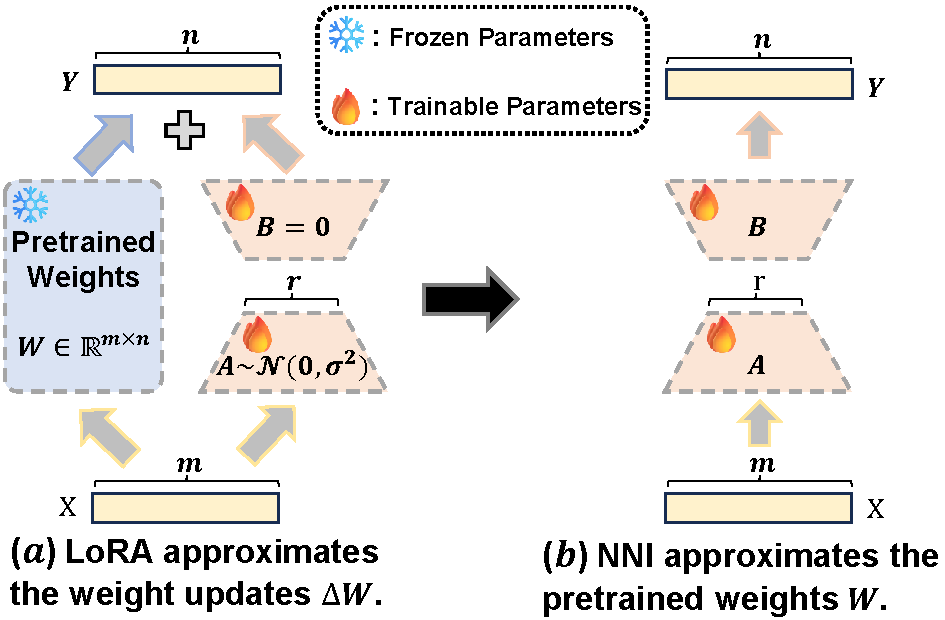
\includegraphics[width=0.5\textwidth]{figures/Motivation.pdf}
    \vspace{-0.6cm}
    \caption{The difference between LoRA and NNI.}
    \label{fig:motivation}
    \vspace{-0.4cm}
\end{wrapfigure}
In recent years, Knowledge Distillation (KD)~\citep{hinton2015distilling} has gained widespread attention and recognition in both academia and industry as an efficient model compression technique~\citep{zhou2018rocket,  xu2024survey}. Its core idea is to transfer knowledge from a large, pretrained teacher network to a lightweight student network, thereby improving the student's performance without significantly increasing additional computational cost. Initially, KD is mainly applied to unimodal tasks, such as visual tasks~\citep{hinton2015distilling, jin2023multi} and textual tasks~\citep{jiao2019tinybert, kang2023distill}. With the advancement of multimodal learning, KD has also been extended to multimodal scenarios for cross-modal knowledge transfer and fusion~\citep{dai2022enabling, yang2024clip}.



However, despite its effectiveness, a widely accepted view is that the performance of student networks is typically inferior to that of teacher networks due to limited capacity~\citep{gou2021knowledge, zhou2025revisiting}. This observation draws a parallel to Parameter-Efficient Fine-Tuning (PEFT)~\citep{mangrulkar2022peft, xu2023parameter, zhou2025cola}, especially the LoRA method~\citep{hu2022lora}. As illustrated in Figure~\ref{fig:motivation} (a), given the pretrained weights $W \in \mathbb{R}^{m \times n}$, LoRA approximates the weight updates $\Delta W$ using a pair of low-rank matrices: $A \in \mathbb{R}^{m \times r}$ (initialized with Gaussian noise) and $B \in \mathbb{R}^{r \times n}$ (initialized with zeros), where $r \ll \min(m, n)$. This approach significantly reduces the number of trainable parameters from $m \times n$ to $r(m + n)$. However, LoRA generally still exhibits a performance gap compared to full fine-tuning~\citep{zhang2023instruction, ding2023parameter, han2024parameter}.




Given \textbf{the strong performance of teacher networks in KD, the difficulty of designing student networks to adapt to the teacher network~\citep{gu2020search, liu2022cross}, and the parameter efficiency of low-rank approximations in LoRA}, we are naturally led to a more affinitive model compression approach: \textit{Neural Network Inheritance} (\textbf{NNI}). Instead of training a separate student network, \textbf{NNI directly inherits the capacity of the teacher network in a low-rank form}. As shown in Figure~\ref{fig:motivation} (b), NNI achieves model compression by performing low-rank decomposition on each layer of the teacher network and replacing the original weights with their decomposed counterparts. Crucially, unlike \textbf{LoRA which approximates weight updates $\Delta W$, InherNet approximates the full pre-trained weights $W$}, preserving the teacher model's expressiveness more directly.


Upon reviewing prior work, we find that a general and widely applicable method for NNI is lacking. \textbf{Existing related efforts are rather fragmented}, mainly focusing on early Convolutional Neural Network (CNN) architectures~\citep{jaderberg2014speeding, zhang2015accelerating, xu2019trained, yang2020learning}, and are mostly confined to vision tasks, with limited applicability to other modalities—particularly the increasingly prominent multimodal tasks. Moreover, \textbf{these methods~\citep{lebedev2014speeding, hu2024dota} often rely on traditional tensor decomposition techniques} (\textit{e.g.}, CP decomposition and MPO decomposition), which break a single layer into multiple sub-layers for compression, \textbf{often making networks deeper and narrower—raising risks of vanishing or exploding gradients and compromising stability and performance}. More importantly, there remains \textbf{a lack of  investigation into the teacher inheritance under KD}, especially in terms of systematically comparing inherited and student networks in performance and efficiency.



To this end, we propose InherNet—a novel and general method for efficiently inheriting the knowledge and structure of teacher networks in KD. For knowledge inheritance, unlike prior decomposition-based methods~\citep{jaderberg2014speeding}, InherNet leverages Singular Value Decomposition (SVD) for initialization (\textbf{SVD offline single-pass computation makes the training time negligible}), allowing the decomposition of only two layers without excessively deepening the network. For structure inheritance, InherNet is \textbf{architecture-agnostic} and applies low-rank approximation to convolutional or linear layers. Previous studies have shown that Mixture of Experts (MoE) models can significantly enhance performance across various tasks~\citep{zhou2022mixture, tian2024hydralora, gao2024higher, cai2024survey}. Inspired by this, InherNet adopts a similar design, enabling both deepening and widening of the network to mitigate the potential risks of gradient vanishing or explosion. This design enables InherNet to remain structurally aligned with the teacher network while also inheriting its representational capacity more faithfully. Notably, our experiments reveal a compelling insight: \textbf{InherNet converges significantly faster than traditional student networks}. We attribute this phenomenon to the extended SVD-based initialization and provide a detailed theoretical analysis to support this claim. Additionally, each layer of the teacher network inherited by InherNet uses a \textbf{fixed} asymmetric design (\textit{i.e.}, a single dimensionality reduction matrix and multiple dimensionality expansion matrices). \textbf{We provide empirical evidence and theoretical support for this fixed design in Appendix~\ref{sec:asymmetric}.}


To summarize, our contributions are in four aspects:
\begin{itemize}
    \item{We propose InherNet, a novel method that explicitly inherits both the knowledge and structure of powerful teacher networks in KD. Unlike implicit knowledge distillation, InherNet constructs a wider, deeper, yet lightweight network without the challenges of heterogeneous knowledge transfer.}
    \item{We uncover and analyze three pivotal insights regarding InherNet, as presented in Sec.~\ref{sec:observation}. These findings illuminate the underlying principles of neural network inheritance and offer clear directions for future research in this area.}
    \item{We provide extensive and rigorous theoretical analysis to explain the empirically observed phenomenon of InherNet's accelerated convergence with comparable parameter sizes. Our proofs formally attribute this efficiency advantage to its SVD-based initialization, establishing a solid theoretical foundation for its design.}
    \item{We conduct systematic experiments across various network architectures and modal tasks, including both unimodal and multimodal scenarios. The results consistently demonstrate that InherNet outperforms traditional student networks in both efficiency and effectiveness.}
\end{itemize}




% 原始的夹型模型在4亿张图像文本对上进行了32个时期的预训练，花费了数千个GPU天。 这给蒸馏带来了重大的成本挑战。
% 在手动继承中，TinyCLIP通过减少图像编码器的宽度和文本编码深度来分别压缩图像编码器和文本编码器

% 总之，提出的继承方法具有：1) 更高的性能。2) 更少的参数。3) 更快的收敛速度。
% 继承网络逆转变换回教师网络

\vspace{-0.2cm}
\section{Methodology}
\label{sec:method}
\setlength{\abovedisplayskip}{3.5pt}
\setlength{\belowdisplayskip}{3.5pt}

\begin{figure*}[t]
    % \vspace{-0.1cm}
    \centering
    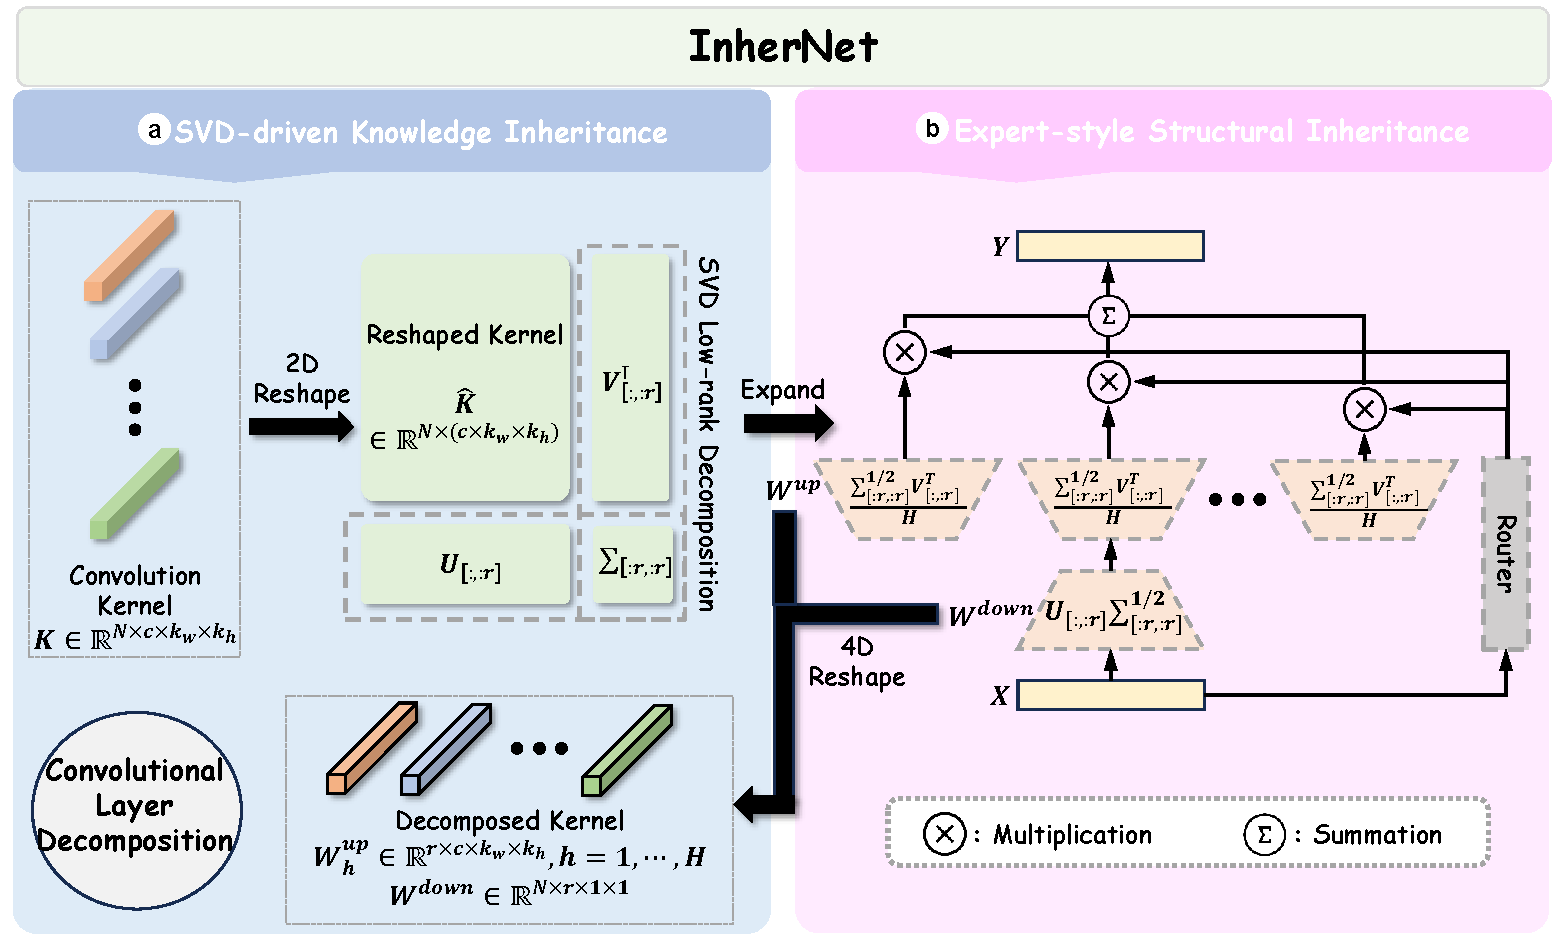
\includegraphics[width=0.8\linewidth]{figures/Method_new.pdf}
    \vspace{-0.3cm}
    \textbf{\caption{Overview of the proposed InherNet (\textit{e.g.}, decomposition of a convolutional layer). InherNet consists of two parts: (a) Knowledge Inheritance and (b) Structure Inheritance. Note that the low-rank decomposition of linear layer is similar, with the key being to satisfy the properties of the 2D SVD operation.}
    \label{fig:method}}
    \vspace{-0.5cm}
\end{figure*}

In this section, we introduce our proposed InherNet method, which consists of knowledge inheritance and structure inheritance, as shown in Figure~\ref{fig:method}. Next, we will provide theoretical analyses of the method's convergence guarantees and parameter efficiency.

% 我们在这一节中介绍我们提出的InherNet方法，其由知识继承和结构继承组成，如图~\ref{fig:method}所示。然后给出我们的方法在收敛速度方面的理论分析。

\subsection{InherNet}


% Recent advances in model compression primarily focus on KD approaches~\citep{hinton2015distilling,gou2021knowledge}, where knowledge from teacher networks is transferred to smaller student networks. Despite their successes, traditional KD methods often face limitations due to a significant capacity gap between the teacher and student networks~\citep{yang2023categories}. Motivated by the parameter efficiency of low-rank optimization~\citep{hu2022lora,meng2024pissa} and the expressive power inherent to pretrained teacher networks, we propose \textit{InherNet}, a novel Neural Network Inheritance (NNI) approach that directly inherits the structure and knowledge of a teacher network via SVD.

\subsubsection{Knowledge Inheritance}

For a linear layer, consider a pretrained teacher network with a weight matrix \( W \in \mathbb{R}^{m\times n} \). InherNet employs SVD to factorize \( W \) into a compact low-rank approximation. Specifically, we have:
\begin{equation}
W = U \Sigma V^\top \approx U_r \Sigma_r V_r^\top,\label{eq:svd}
\end{equation}

where \( U_r \in \mathbb{R}^{m\times r} \), \(\Sigma_r \in \mathbb{R}^{r\times r}\), and \( V_r \in \mathbb{R}^{n\times r} \) represent truncated matrices derived from the top-\( r \) singular values and vectors. Therefore, the original layer is approximated by two consecutive low-rank layers, $U_r\Sigma_r$ and $\Sigma_r V_r^\top$. The approximation is supported by Theorem~\ref{thm:young}.

% \begin{theorem}\label{thm:young}
% If the SVD of $W \in \mathbb{R}^{n \times m}$ is $U \Sigma V^{\top}$, then the optimal rank- $r$ approximation of $W$ is $U_{[:n, :r]} \Sigma_{[: r, :r]} V_{[:m, :r]}^{\top}$.
% \end{theorem}
\begin{theorem}[Eckart-Young-Mirsky theorem]\label{thm:young}
Given a weight matrix \( W \in \mathbb{R}^{m \times n} \) with singular value decomposition \( W = U \Sigma V^\top \), the optimal rank-\( r \) approximation in terms of Frobenius norm is given by: \(W_r = U_{[:, :r]} \Sigma_{[:r, :r]} V_{[:, :r]}^\top\). Moreover, the approximation error is minimized, specifically:
\begin{equation}
\|W - W_r\|_F = \sqrt{\sum_{i=r+1}^{\min(m,n)}\sigma_i^2(W)},
\end{equation}
where \(\sigma_i(W)\) denotes the \(i\)-th singular value of \(W\)~\citep{golub1987generalization,eckart1936approximation,golub2013matrix}.
\end{theorem}

For a convolutional layer, as shown in Figure~\ref{fig:method} (a), formally, there exists a convolution kernel $K \in \mathbb{R}^{N \times c \times k_w \times k_h}$, where $n, c, k_w, k_h$ represent the number of kernels, the number of input channels, and the width and height of the filter, respectively. Our work focuses on the channel decomposition method~\citep{zhang2015accelerating} to decompose the convolution layer. Specifically, $K$ is first reshaped into a 2D matrix $\hat{K} \in \mathbb{R}^{N \times (c \times k_w \times k_h)}$, and SVD initialization is applied. The resulting decomposed layers are reshaped to have convolutional kernel weights $W^{down} \in \mathbb{R}^{N \times r \times 1 \times 1}$ and $W^{up} \in \mathbb{R}^{r \times c \times k_w \times k_h}$.

% 对于一个卷积层$\mathcal{L}_i$，如图~\ref{fig:method}~(a)所示，形式上，一个卷积滤波器$K$可以通过一个张量表示: $W\in \mathbb{R}^{n\times c\times w\times h}$，这里$n, c, w, h$分别表示滤波器的数量、输入通道的数量、滤波器的宽度和高度。我们的工作主要关注通道分解方法~\citep{zhang2015accelerating}来分解卷积层，即$K$首先被重塑为一个二维矩阵$\hat{K}\in \mathbb{R}^{n\times (c\times w\times h)}$，然后对其执行SVD初始化，得到的分解层重塑后分别具有卷积核权重$W^{down}\in \mathbb{R}^{n\times r \times 1 \times 1}$和$W^{up}\in \mathbb{R}^{r\times c \times w \times h}$。

\subsubsection{Structure Inheritance}

Unlike previous low-rank decomposition methods~\citep{jaderberg2014speeding, zhang2015accelerating, zhou2025cuff}, we adopt an expert-style inheritance structure inspired by the Mixture of Experts (MoE) paradigm, which has been widely proven effective across various domains~\citep{tian2024hydralora, gao2024higher, cai2024survey}. As illustrated in Figure~\ref{fig:method} (b), in order to strike a good balance between performance and efficiency, we design an asymmetric expert-head structure. Specifically, given input features $X\in \mathbb{R}^m$, the output $Y\in \mathbb{R}^n$ of InherNet is formulated as:

\begin{equation}
Y = \sum_{h=1}^{H} G_h(X) \cdot W^{up}_h\left(W^{down}(X)\right),
% \label{eq:one_down}
\end{equation}
where \(H\) denotes the number of expert heads, \(W^{down}\) and \(W^{up}_h\) represent the ``down'' projection of the backbone branch and the ``up'' projection of the \(h\)-th expert head, respectively. $W^{down}$ and $W^{up}_h$ are initialized using $U_{[:, :r]}\Sigma_{[:r,:r]}^{1/2}$ and $\frac{\Sigma_{[:r,:r]}^{1/2}V_{[:,:r]}^\top}{H}$ from Eq.~\ref{eq:svd}, and the matrix slicing notations follow the same convention as in PyTorch. \(G(X)\) represents adaptive gating fusion weights computed as:
\begin{equation}
G(X) = \text{softmax}\left(W^g(X)\right),
\end{equation}
where $W^g\in \mathbb{R}^{m\times H}$ is a learnable parameter.

% To enhance the representational flexibility, we introduce a multi-head decomposition inspired by Mixture of Experts (MoE)~\citep{cai2024survey}. Instead of a single reconstruction, we initialize multiple lightweight heads based on the SVD decomposition. Specifically, the decomposition includes two steps:

% \textbf{Embedding Step:} The original input is embedded into a low-dimensional space through a compressed transformation initialized from \( V_r^\top \).

% \textbf{Multi-Head Reconstruction Step:} Multiple parallel expert heads, initialized using the truncated matrices \(U_r \Sigma_r\), independently reconstruct output features.

% To dynamically aggregate information from multiple heads, we introduce an adaptive gating network. This gating mechanism computes soft weighting coefficients based on input context, allowing the network to select the most effective combination of experts during inference. Given input features \( X \), the output \( Y \) of InherNet is formulated as:
% \begin{equation}
% Y = \sum_{h=1}^{H} G_h(X) \cdot \mathcal{F}^{(h)}_{\text{head}}\left(\mathcal{F}_{\text{embed}}(X)\right),
% \end{equation}
% where \(H\) denotes the number of heads, and \(G_h(X)\) represents adaptive gating weights computed as: \(G(X) = \text{softmax}\left(\phi(\text{GAP}(X))\right)\). Here, \(\text{GAP}(\cdot)\) denotes global average pooling, and \(\phi(\cdot)\) is a tiny learnable fully connected layer.

The InherNet's procedure can be found in Appendix~\ref{app:algo}. We also provide empirical and theoretical support for InherNet's fixed asymmetric structural design in Appendix~\ref{sec:asymmetric}. Note that InherNet inherently benefits from SVD and gating mechanism, theoretically enabling excellent convergence and parameter efficiency, as rigorously analyzed in Sec.~\ref{sec:convergence} and Sec.~\ref{sec:parameter}. By directly inheriting structural knowledge through decomposition and adaptively aggregating expert heads, InherNet provides an efficient and expressive solution, as demonstrated by our experiments in Sec.~\ref{sec:experiments}.

% \begin{algorithm}[!htbp]
%     \caption{InherNet: SVD-Driven Neural Network Inheritance}
%     \label{alg:inhernet}
%     \begin{algorithmic}[1]
%         \REQUIRE Pretrained teacher weight \(W \in \mathbb{R}^{m \times n}\), rank \(r\), number of heads \(H\), input \(X\)
%         \ENSURE Output \(Y\)

%         \STATE Perform truncated SVD: \(W \approx U_r\Sigma_r V_r^\top\).
%         \STATE Set backbone branch: \(W^{down}(\cdot)\leftarrow U_r \Sigma_r^{1/2}\).
%         \FOR{\(h=1,2,\dots,H\)}
%             \STATE Set \textit{h}-th head: \(W^{up}_{h}(\cdot)\leftarrow \frac{1}{H} \Sigma_r^{1/2} V_r^\top\).
%         \ENDFOR

%         \STATE Compute backbone branch output: \(X_r = W^{down}(X)\).
%         \FOR{\(h=1,2,\dots,H\)}
%             \STATE Compute expert head outputs: \(Z^{(h)} = W^{up}_h(X_r)\).
%         \ENDFOR

%         \STATE Compute gating weights: \(G(X)=\text{softmax}\left(W^g(X)\right)\).

%         \STATE Aggregate outputs dynamically: \(Y=\sum_{h=1}^{H}G_h(X)\cdot Z^{(h)}\)


%         \RETURN \(Y\)
%     \end{algorithmic}
% \end{algorithm}



\subsection{Theoretical Analysis of Convergence Guarantees}
\label{sec:convergence}

We analyze the convergence properties of InherNet, focusing on its structured low-rank decomposition, multi-head gating mechanism, and SVD-based initialization. Our goal is to establish that, despite the compression from low-rank projections, InherNet has stable and efficient optimization under stochastic gradient descent (SGD).

Let $\mathcal{L}(\theta) = \mathbb{E}_{(x,y)\sim \mathcal{P}}[\ell(f_\theta(x), y)]$ be the expected loss, where $(x, y) \sim \mathcal{P}$ denotes data sampled from the underlying distribution. Let $\theta \in \mathbb{R}^d$ denote the parameters of an InherNet, and let $\theta^{(t)}$ be the model parameters at iteration $t$ updated via stochastic gradients.

We impose the following assumptions, which are common in the analysis of stochastic optimization for nonconvex problems~\citep{patel2022global, xu2024psmgd, lei2019stochastic, pham2020proxsarah}:

\begin{assumption}[Lipschitz Continuity]
\label{assumption:lipschitz}
The expected loss gradient is $L$-Lipschitz continuous:
\begin{equation}
    \|\nabla \mathcal{L}(\theta) - \nabla \mathcal{L}(\theta')\| \leq L\|\theta - \theta'\|, \quad \forall \theta, \theta' \in \mathbb{R}^d.
\end{equation}
\end{assumption}

\begin{assumption}[Bounded Variance]
\label{assumption:variance}
The stochastic gradient $\nabla_\theta \ell(f_\theta(x), y)$ is unbiased and has bounded variance:
\begin{equation}
    \mathbb{E}[\nabla_\theta \ell(f_\theta(x), y)] = \nabla \mathcal{L}(\theta), \quad
\mathbb{E}\left[\left\|\nabla_\theta \ell - \nabla \mathcal{L}(\theta)\right\|^2\right] \leq \sigma^2.
\end{equation}
\end{assumption}

\begin{assumption}[Bounded Representations]
\label{assumption:bounded}
There exist constants $B_x, B_f > 0$ such that $\|x\| \leq B_x$ and $\|f_\theta(x)\| \leq B_f$ for all $(x,y)\sim \mathcal{P}$.
\end{assumption}

\subsubsection{Gradient Decomposition under InherNet}

InherNet models each module as a low-rank gated composition:
\begin{equation}
f_\theta(x) = \sum_{h=1}^H G_h(x;\theta_g)\, W^{\text{up}}_h(W^{\text{down}}(x)),
\end{equation}
where $W^{\text{down}}$ is the shared projection, $W^{\text{up}}_h$ is the $h$-th expert head, and $G_h(.)$ is a gating weight.


% \begin{lemma}[Gradient Decomposition]
% \label{lemma:gradient-decomposition}
% Total gradient $\nabla_\theta \ell(f_\theta(x), y)$ decomposes into two additive components:
% \begin{equation}
% \nabla_\theta \ell = \sum_{h=1}^H G_h(x)\, \nabla_{\theta_h} \ell + \sum_{h=1}^H \Delta_h\, \nabla_{\theta_g} G_h(x),
% \end{equation}
% where $\theta_h$ and $\theta_g$ are the parameters of expert head $h$ and the gating network, respectively, and $\Delta_h = \frac{\partial \ell}{\partial f_h(x)}$.
% \end{lemma}
\begin{lemma}[Gradient Decomposition]
\label{lemma:gradient-decomposition}
Under the InherNet parameterization, the gradient of the loss splits naturally into contributions from each head and from the gating network. The total gradient $\nabla_\theta \ell(f_\theta(x), y)$ decomposes into:
\begin{equation}
\begin{aligned}
\nabla_\theta \ell\!\bigl(f_\theta(x),y\bigr)
&= \sum_{h=1}^H G_h\!\bigl(x;\theta_g\bigr)\,\nabla_{\theta_h}\ell\!\bigl(f_\theta(x),y\bigr) + \sum_{h=1}^H \Delta_h\,\nabla_{\theta_g} G_h\!\bigl(x;\theta_g\bigr),
\end{aligned}
\end{equation}
where $\theta_h$ and $\theta_g$ are the parameters of expert head $h$ and the gating network, respectively, and $\Delta_h = \frac{\partial \ell(f_\theta(x),y)}{\partial f_h(x)}$ represents the gradient of the loss with respect to the output of the $h$-th head, with $f_h(x) = W^{\text{up}}_h(W^{\text{down}}(x))$.
\end{lemma}

This gradient routing allows InherNet to specialize experts during training, directing gradient flow to the most relevant parameters for each input. It is beneficial when compressing teacher networks.

\subsubsection{Effect of SVD-Based Initialization and Convergence Guarantee}

Let $W$ denote the pretrained weight from a teacher network. InherNet initializes each module using truncated SVD. The initialized parameters are: \(W^{\text{down}} = U_r \Sigma_r^{1/2}, \quad W^{\text{up}}_h = \frac{1}{H} \Sigma_r^{1/2} V_r^\top.\)

\begin{proposition}[Stability via Orthonormal Initialization]
\label{prop:stability}
If $U_r$ and $V_r$ are initialized with orthonormal columns, then under Assumption~\ref{assumption:lipschitz}, the effective gradient Lipschitz constant is reduced from $L$ to $L' \approx L / \kappa$, where $\kappa$ is the condition number of $W$.
\end{proposition}

This improved conditioning reduces curvature imbalance during early training and stabilizes convergence, particularly when the teacher model is well-trained~\citep{wang2024model, lim2024simple, saxe2013exact}.

% \subsubsection{Convergence Guarantee}

\begin{theorem}[Non-Convex Convergence]
\label{thm:convergence}
Under Assumptions~\ref{assumption:lipschitz}--\ref{assumption:bounded}, and adopting a diminishing learning rate schedule $\eta_t = \frac{\eta}{\sqrt{t}}$, the sequence of parameters $\{\theta^{(t)}\}$ generated by InherNet satisfies the following convergence rate:
\begin{equation}
    \frac{1}{T}\sum_{t=1}^{T}\mathbb{E}\left[\|\nabla\mathcal{L}(\theta^{(t)})\|^2\right]=\mathcal{O}\left(\frac{1}{\sqrt{T}}\right).
\end{equation}
\end{theorem}


The convergence rate matches classical result for non-convex optimization problems~\citep{xu2024psmgd}. Because of the SVD-based orthonormal initialization and adaptive gating mechanism, InherNet achieves convergence rate of $\mathcal{O}(1/\sqrt{T})$ with practical scaling as $\mathcal{O}(L/\kappa)$. The improved convergence behavior stems from Proposition~\ref{prop:stability}, where the Lipschitz constant for gradient updates is reduced from $L$ to $L' \approx L/\kappa$. This reduction in curvature imbalance commits to lower gradient variance and faster gradient descent in early stages, as empirically verified in Sec.~\ref{sec:observation}.

% \begin{itemize}[leftmargin=*, topsep=2pt, itemsep=2pt]
%   \item \textbf{Full-rank Networks}: A full-rank network achieves $\mathcal{O}(1/\sqrt{T})$ convergence with constants that scale as $\mathcal{O}(L)$, where $L$ is proportional to the condition number $\kappa$ of the original weight matrices, causing slower practical convergence.
  
%   \item \textbf{LoRA}~\citep{hu2022lora}: Although LoRA achieves the same theoretical convergence rate $\mathcal{O}(1/\sqrt{T})$, it typically inherits the poor conditioning of the original network since it lacks explicit orthonormal initialization, thereby limiting practical convergence speed~\citep{yuan2024bridging,qin2024convergence}.
  
%   \item \textbf{InherNet (Proposed)}: Due to the SVD-based orthonormal initialization and adaptive gating mechanism, InherNet achieves a convergence rate of $\mathcal{O}(1/\sqrt{T})$ with practical constants scaling as $\mathcal{O}(L/\kappa)$. Thus, InherNet theoretically improves practical convergence speed by a factor proportional to the condition number $\kappa$, enhancing early-phase training stability and efficiency.
% \end{itemize}

% The improved convergence behavior stems primarily from Proposition~\ref{prop:stability}, where the Lipschitz constant for gradient updates is effectively reduced from $L$ to $L' \approx L/\kappa$. This reduction in curvature imbalance directly translates into lower gradient variance and faster gradient descent, especially in the initial stages of training, as empirically verified in Observation 3 in Sec.~\ref{sec:observation}.

% \begin{remark}[Convergence in Different Optimization Regimes]
% Our analysis primarily addresses non-convex optimization scenarios, as these are most relevant for training neural networks. Nonetheless, the convergence guarantees provided by InherNet naturally extend to other standard optimization scenarios:
% \begin{itemize}[leftmargin=*, topsep=2pt, itemsep=2pt]
%     \item For general convex objectives, InherNet achieves the standard SGD rate of $\mathcal{O}(1/T)$, but with improved constants due to orthonormal initialization.
%     \item In $\mu$-strongly convex settings, InherNet achieves an exponential convergence rate of $\mathcal{O}(e^{-\eta\mu T})$ for a learning rate $\eta$, with significant improvements arising again from orthonormal parameter initialization.
% \end{itemize}
% \end{remark}


% \subsubsection{Convergence Guarantee}

% \begin{theorem}[Non-Convex Convergence]
% \label{thm:convergence}
% Under Assumptions~\ref{assumption:lipschitz}–\ref{assumption:bounded}, and using a learning rate schedule $\eta_t = \eta / \sqrt{t}$, the parameter sequence $\{\theta^{(t)}\}$ produced by InherNet satisfies:
% \begin{equation}
%     \frac{1}{T} \sum_{t=1}^T \mathbb{E}[\|\nabla \mathcal{L}(\theta^{(t)})\|^2] = \mathcal{O}\left(\frac{1}{\sqrt{T}}\right).
% \end{equation}
% \end{theorem}

% While this matches the asymptotic rate for SGD in non-convex settings, the specific convergence properties differ substantially between methods:

% \begin{itemize}
%   \item \textbf{Full-rank networks}: Under standard initialization, a full-rank network achieves $\mathcal{O}(1/\sqrt{T})$ convergence with constants that scale as $\mathcal{O}(L)$, where $L \propto \kappa$ (the condition number of weight matrices). This results in slow practical convergence.
  
%   \item \textbf{LoRA}~\citep{hu2022lora}: Achieves $\mathcal{O}(1/\sqrt{T})$ convergence but operates only within restricted low-rank subspaces. And it inherits the conditioning issues of the original weight space, as it lacks explicit orthogonalization in its parameterization~\citep{yuan2024bridging}.
  
%   \item \textbf{DeepLinearNet}~\citep{saxe2013exact}: Achieves $\mathcal{O}(1/\sqrt{T})$ convergence with improved constants via orthogonal initialization, but lacks gating and non-linearity.
  
%   \item \textbf{InherNet}: Achieves $\mathcal{O}(1/\sqrt{T})$ convergence with constants that scale as $\mathcal{O}(L/\kappa)$ due to orthonormal initialization from SVD. This yields a theoretical speedup factor of $\kappa$ in early convergence while maintaining parameter efficiency through decomposition and adaptive multi-head design.
% \end{itemize}

% For InherNet, the Lipschitz constant of the compressed parameterization is $L' \approx L/\kappa$ (per Proposition~\ref{prop:stability}), leading to reduced gradient variance and faster descent in the initial training phase. This theoretical advantage is confirmed in Sec.~\ref{sec:experiments}.

% \begin{remark}[Convergence in Different Optimization Regimes]
% While our analysis focuses on the non-convex case most relevant to neural networks, the convergence properties of InherNet extend to other optimization regimes with the following guarantees:

% \begin{itemize}
%     \item For convex functions, under the same assumptions and learning rate schedule, InherNet would achieve the standard $\mathcal{O}(1/T)$ convergence rate with improved constants due to SVD-based initialization.
    
%     \item For $\mu$-strongly convex functions, the convergence rate would improve to $\mathcal{O}((1-\eta\mu)^T)$ or equivalently $\mathcal{O}(e^{-\eta\mu T})$ for appropriate learning rate $\eta$, again with conditioning benefits from orthonormal initialization.
% \end{itemize}
% \end{remark}


% \subsubsection*{Summary}

% Despite its low-rank parameterization, InherNet preserves expressive optimization dynamics via gated expert structures and principled SVD-based initialization. Theoretical convergence guarantees match those of unconstrained SGD, while improved conditioning and adaptive gradient flow explain the method's superior convergence and robustness.

% \subsubsection*{Comparison with other compression methods}

% LoRA~\citep{hu2021lora} introduces additive low-rank adapters to frozen pretrained layers and requires manually tuned rank schedules and training heuristics. It does not modify the main weight matrix and often requires auxiliary regularization for stability. In contrast, InherNet directly inherits structural priors from the teacher via truncated SVD, enabling a stable and expressive parameterization without freezing or decoupling.

% DeepLinearNet~\citep{saxe2013exact} shows that linear deep networks with orthogonal initialization can achieve optimal conditioning, but its theory assumes fixed architectures without gating or compositionality. InherNet generalizes this structure by supporting dynamic, gated multi-head routing with non-linear activations, yielding both richer expressiveness and empirically faster convergence.


% \subsection{InherNet: Neural Network Inheritance via Low-Rank Decomposition}

% Recent advances in model compression primarily focus on knowledge distillation (KD) approaches~\citep{hinton2015distilling,gou2021knowledge}, where knowledge from large teacher networks is transferred to smaller student networks. Despite their successes, traditional KD methods often face limitations due to a significant capacity gap between the teacher and student models~\citep{yang2023categories}. Motivated by the parameter efficiency of Low-Rank Adaptation (LoRA)~\citep{hu2022lora,meng2024pissa} and the expressive power inherent to pretrained teacher networks, we propose \textit{InherNet}, a novel Neural Network Inheritance (NNI) approach that directly inherits the structure and knowledge of a teacher network via SVD.

% Consider a pretrained teacher network with a weight matrix \( W \in \mathbb{R}^{m\times n} \). InherNet employs SVD to factorize \( W \) into a compact low-rank approximation. Specifically, we have:
% \[
% W = U \Sigma V^\top \approx U_r \Sigma_r V_r^\top,
% \]
% where \( U_r \in \mathbb{R}^{m\times r} \), \(\Sigma_r \in \mathbb{R}^{r\times r}\), and \( V_r \in \mathbb{R}^{n\times r} \) represent truncated matrices derived from the top-\( r \) singular values and vectors.

% To enhance the representational flexibility, we introduce a multi-head decomposition inspired by Mixture of Experts (MoE)~\citep{cai2024survey}. Instead of a single reconstruction, we initialize multiple lightweight heads based on the SVD decomposition. Specifically, the decomposition includes two steps:

% \textbf{Embedding Step:} The original input is embedded into a low-dimensional space through a compressed transformation initialized from \( V_r^\top \).

% \textbf{Multi-Head Reconstruction Step:} Multiple parallel expert heads, initialized using the truncated matrices \(U_r \Sigma_r\), independently reconstruct output features.

% To dynamically aggregate information from multiple heads, we introduce an adaptive gating network. This gating mechanism computes soft weighting coefficients based on input context, allowing the network to select the most effective combination of experts during inference. Given input features \( X \), the output \( Y \) of InherNet is formulated as:
% \begin{equation}
% Y = \sum_{h=1}^{H} G_h(X) \cdot \mathcal{F}^{(h)}_{\text{head}}\left(\mathcal{F}_{\text{embed}}(X)\right),
% \end{equation}
% where \(H\) denotes the number of heads, and \(G_h(X)\) represents adaptive gating weights computed as: \(G(X) = \text{softmax}\left(\phi(\text{GAP}(X))\right)\). Here, \(\text{GAP}(\cdot)\) denotes global average pooling, and \(\phi(\cdot)\) is a tiny learnable fully connected layer.

% The full procedure of InherNet is shown in Algorithm~\ref{alg:inhernet}. InherNet inherently benefits from the orthogonality constraints imposed by SVD, theoretically enabling stable initialization and faster convergence, as rigorously analyzed in Subsection 3.2 and 3.3. By directly inheriting structural knowledge through SVD decomposition and adaptively aggregating expert heads, InherNet provides an efficient and expressive solution, as demonstrated by our experiments in Sec.~4.


\subsection{Theoretical Proof of Parameter Efficiency}
\label{sec:parameter}

We analyze parameter efficiency of InherNet, establishing theoretical guarantees on both parameter reduction and representational power preservation. Our analysis formalizes the efficiency-expressivity tradeoff through three metrics:

\begin{definition}[Parameter Efficiency (PE)]\label{def:pe_}
For network $f_\theta$ parameterized by $\theta \in \mathbb{R}^p$, we define $\text{PE}(f_\theta) = \frac{\text{Representational Capacity}(f_\theta)}{|\theta|}$. Representational capacity measures the network's approximation ability and $|\theta|$ denotes parameter count.
\end{definition}

\begin{definition}[Approximation Error]\label{def:approx-error_}
Given a target function $f^*$ and a neural network $f_\theta$, the approximation error is 
$\mathcal{E}(f_\theta, f^*) = \mathbb{E}_{x \sim \mathcal{D}}[\|f_\theta(x) - f^*(x)\|^2]$,
where $\mathcal{D}$ is the data distribution.
\end{definition}

\begin{definition}[Expressivity-to-Parameter Ratio (EPR)]\label{def:epr_}
The EPR of network $f_\theta$ with respect to function class $\mathcal{F}$ is 
$\text{EPR}(f_\theta, \mathcal{F}) = \frac{1}{|\theta|\inf_{f^* \in \mathcal{F}} \mathcal{E}(f_\theta, f^*)}$,
measuring the inverse of minimum achievable approximation error per parameter.
\end{definition}

\subsubsection{Compression Bounds for InherNet}

We first quantify the parameter reduction achieved by InherNet relative to a standard network, which directly improves the PE as defined in Definition~\ref{def:pe_}.

\begin{theorem}[Parameter Reduction Bounds]
\label{thm:reduction_}
Consider a layer \(W\in\mathbb R^{m\times n}\).  The InherNet parameterization with rank \(r\) and \(H\) heads uses $H\,r\,(m+n)\;+\;H\,(r+1)$ trainable parameters, yielding a compression ratio:
\begin{equation}
\rho
=\;
\frac{m\,n}
     {H\,r\,(m+n) + H\,(r+1)}
=\;
\frac{m\,n}
     {H\,r\,(m+n)}
\Bigl(1+O\bigl(\tfrac1{m+n}\bigr)\Bigr)
\end{equation}
Thus, it achieves an approximately \(\rho\)-fold increase in Definition~\ref{def:pe_}, under the assumption that a rank-\(H\,r\) subspace preserves the layer's representational capacity.
\end{theorem}

To ensure low Approximation Error (Definition~\ref{def:approx-error_}) despite compression, we establish:

\begin{lemma}[Spectral Energy Preservation]\label{lem:spectral_}
Let $W \in \mathbb{R}^{m \times n}$ have singular values $\sigma_1 \ge \sigma_2 \ge \cdots \ge \sigma_{\min(m,n)}$. If the rank $r$ is selected such that:
\begin{equation}
\frac{\sum_{i=1}^{r} \sigma_i^2}{\sum_{i=1}^{\min(m,n)} \sigma_i^2} \ge 1 - \epsilon
\end{equation}
then by Theorem~\ref{thm:young}, the Frobenius-norm error of the optimal rank-$r$ approximation $W_r$ is bounded by: \(\|W - W_r\|_F^2 \leq \epsilon\|W\|_F^2\).
% \begin{equation}
% \|W - W_r\|_F^2 \leq \epsilon\|W\|_F^2
% \end{equation}
Consequently, the Definition~\ref{def:approx-error_} between an InherNet-compressed layer and the original layer is bounded by $\epsilon$ under the $L_2$ norm squared.
\end{lemma}

\begin{proposition}[Knowledge Preservation Rate]\label{prop:knowledge-preservation_}
Let $f_W$ be a teacher network with weight matrices $\{W_l\}$ and $f_r$ be the corresponding InherNet with rank $r$. The functional similarity between $f_W$ and $f_r$ is lower-bounded by:
\begin{equation}
\text{Sim}(f_W, f_r) \geq 1 - \sum_{l=1}^L \alpha_l \left(1 - \frac{\sum_{i=1}^{r} \sigma_{l,i}^2}{\sum_{i=1}^{\min(m_l,n_l)} \sigma_{l,i}^2}\right)
\end{equation}
where $\alpha_l$ represents the layer's influence on output, and $\sigma_{l,i}$ are the singular values of $W_l$. This bound is monotonically increasing with $r$ but not with $H$, establishing that rank is the primary metric of inherited knowledge preservation.
\end{proposition}

\subsubsection{Representational Power Preservation}

InherNet also maintains the representational power of the original network, preserving a beneficial EPR (Definition~\ref{def:epr_}):

\begin{theorem}[Representational Power Preservation]\label{thm:rep-power_}
Let $\mathcal{F}_W$ be functions representable by a standard network with weights $\{W_l\}_{l=1}^L$. For any $f^* \in \mathcal{F}_W$ and $\delta > 0$, there exists an InherNet network with appropriate ranks $\{r_l\}$ and head counts $\{H_l\}$ such that the Approximation Error (Definition~\ref{def:approx-error_}) satisfies:
\begin{equation}
\mathcal{E}(f_{\text{InherNet}}, f^*) \le \delta
\end{equation}
while the parameter count is reduced by $\Omega(\min_{l} \frac{\min(m_l,n_l)}{r_l H_l})$ relative to the standard network. Consequently, the InherNet architecture attains an EPR (Definition~\ref{def:epr_}) higher than that of the standard architecture by at least the same factor.
\end{theorem}

This preservation stems from two complementary mechanisms:
1. \textbf{Layer-wise low-rank approximation:} Capturing the dominant spectral components of each weight matrix;
2. \textbf{Multi-head specialization:} Allowing different heads to specialize on different input subspaces.

\begin{corollary}[Universal Approximation]\label{cor:universal_}
InherNet retains the universal function approximation property of standard neural networks while using asymptotically fewer parameters. For any continuous target function, a sufficiently large InherNet network can approximate it arbitrarily well (to Approximation Error $\delta \to 0$) with significantly higher Parameter Efficiency and EPR than a standard network of comparable accuracy.
\end{corollary}

% \subsubsection{Optimal Parameter Allocation}

% We establish principles for optimally allocating parameters across layers to maximize the EPR:

% \begin{theorem}[Optimal Parameter Distribution]\label{thm:optimal-allocation}
% Under a fixed parameter budget $C$, the optimal allocation between layers $i$ and $j$ satisfies:
% \begin{equation}
% \frac{r_i H_i}{r_j H_j} \approx \sqrt{\frac{m_i n_i \lambda_i}{m_j n_j \lambda_j}}
% \end{equation}
% where $\lambda_l$ represents layer $l$'s sensitivity coefficient—the marginal contribution of this layer's approximation error to the overall network performance.
% \end{theorem}

% \begin{corollary}[Rank–Head Trade-off]\label{cor:rank-vs-head}
% Given a fixed parameter budget for a single layer, the optimal trade-off between the rank $r$ and number of heads $H$ depends on the diversity of patterns in the layer's input. Specifically, for input distributions with high diversity or multiple modes, increasing $H$ at the expense of a smaller $r$ yields lower approximation error.
% \end{corollary}

% Please add the following required packages to your document preamble:
% \usepackage{booktabs}
% \usepackage{multirow}
% \usepackage{graphicx}
\begin{table*}[th!]
\centering
% \setlength{\tabcolsep}{0.4mm}

\caption{Comparison of top-1 Accuracy (\%) on the CIFAR-100 validation set between InherNet and previous state-of-the-art knowledge distillation methods. \textbf{Best results} are in bold, and the \underline{second-best} are underlined.}
\label{tab:cifar}
\vspace{-0.3cm}
\resizebox{\columnwidth}{!}{
\begin{tabular}{@{}c|c|ccccccc@{}}
\toprule[1.3pt]
\multirow{4}{*}{KD Type}     & \multirow{2}{*}{Teacher} & ResNet32$\times 4$ & VGG13 & WRN-40-2 & WRN-40-2 & ResNet56 & ResNet110 & ResNet110 \\
                          &                          & 79.42              & 74.64 & 75.61    & 75.61    & 72.34    & 74.31     & 74.31     \\ \cmidrule(l){2-9} 
                          & \multirow{2}{*}{Student} & ResNet8$\times 4$  & VGG8  & WRN-40-1 & WRN-16-2 & ResNet20 & ResNet32  & ResNet20  \\
                          &                          & 72.50              & 70.36 & 71.98    & 73.26    & 69.06    & 71.14     & 69.06     \\ \midrule
\multirow{5}{*}{Feature}  & CRD                      & 75.51              & 73.94 & 74.14    & 75.48    & 71.16    & 73.48     & 71.46     \\
                          & OFD                      & 74.95              & 73.95 & 74.33    & 75.24    & 70.98    & 73.23     & 71.29     \\
                          & ReviewKD                 & 75.63              & 74.84 & 75.09    & 76.12    & 71.89    & 73.89     & 71.34     \\
                          & SimKD                    & 78.08              & 74.89 & 74.53    & 75.53    & 71.05    & 73.92     & 71.06     \\
                          & CAT-KD                   & 76.91              & 74.65 & 74.82    & 75.60    & 71.62    & 73.62     & 71.37     \\ \midrule
\multirow{5}{*}{Logit}    & KD                       & 73.33              & 72.98 & 73.54    & 74.92    & 70.66    & 73.08     & 70.67     \\
                          & KD+CTKD                  & 73.39              & 73.52 & 73.93    & 75.45    & 71.19    & 73.52     & 70.99     \\
                          & DKD                      & 76.32              & 74.68 & 74.81    & 76.24    & 71.97    & 74.11     & 71.06     \\
                          & MLKD                     & 77.08              & 75.18 & 75.35    & \underline{76.63}    & 72.19    & 74.11     & 71.89     \\
                          & MLKD+Logit Std.          & \underline{78.28}
                          & \underline{75.22} & 75.56    & \textbf{76.95}    & 72.33    & \underline{74.32}     & 72.27     \\ \midrule
\multirow{2}{*}{InherNet} & Small                    & 77.57              & \textbf{75.68} & \underline{76.04}    & 76.04    & \underline{72.67}    & 74.13     & \underline{74.13}     \\ \cmidrule(l){2-9} 
                          & Large                    & \textbf{78.53}              & 75.16 & \textbf{76.39}    & 76.39    & \textbf{73.67}    & \textbf{75.88}     & \textbf{75.88}     \\ \bottomrule[1.3pt]
\end{tabular}%
}

\vspace{-0.5cm}
\end{table*}

\begin{proposition}[Diminishing Returns of Multiple Heads]\label{prop:head-diminishing_}
For a given layer with rank $r$, the marginal reduction in approximation error from adding the $(H+1)$-th head satisfies:
\begin{equation}
\mathcal{E}(r,H) - \mathcal{E}(r,H+1) \leq \frac{c}{H^2}\mathcal{E}(r,1)
\end{equation}
where $c$ is a constant depending on input distribution characteristics, and $\mathcal{E}(r,H)$ denotes the approximation error with rank $r$ and $H$ heads. This establishes that benefits from additional heads diminish at a rate of $\Omega(1/H^2)$.
\end{proposition}

The theoretical results explain empirical insights in Sec.~\ref{sec:observation}: (1) rank plays the primary role in preserving teacher knowledge as formalized in Proposition~\ref{prop:knowledge-preservation_}, and (2) while multiple heads outperform a single head, adding more heads yields diminishing returns as quantified in Proposition~\ref{prop:head-diminishing_}. \textbf{Detailed theoretical proofs and extended discussions are provided in Appendix~\ref{app:all}}.

% \subsection{Theoretical Proof of Parameter Efficiency}
% \label{sec:parameter}

% We analyze the parameter efficiency of InherNet, establishing theoretical guarantees on parameter reduction and preservation of representational capacity despite compression. We formalizes the efficiency-expressivity tradeoff through key metrics defined below:

% \begin{definition}[Parameter Efficiency (PE)]\label{def:pe_}
% For a network $f_\theta$ parameterized by $\theta \in \mathbb{R}^p$, we define $\text{PE}(f_\theta) = \frac{\text{Representational Capacity}(f_\theta)}{|\theta|}$. Representational capacity measures the approximation ability and $|\theta|$ denotes parameter count.
% \end{definition}

% \begin{definition}[Approximation Error]\label{def:approx-error_}
% Given a target function $f^*$ and a neural network $f_\theta$, the approximation error is 
% $\mathcal{E}(f_\theta, f^*) = \mathbb{E}_{x \sim \mathcal{D}}[\|f_\theta(x) - f^*(x)\|^2]$,
% where $\mathcal{D}$ is the data distribution.
% \end{definition}

% \begin{definition}[Expressivity-to-Parameter Ratio (EPR)]\label{def:epr_}
% The EPR of network $f_\theta$ with respect to function class $\mathcal{F}$ is 
% $\text{EPR}(f_\theta, \mathcal{F}) = \frac{1}{|\theta|\inf_{f^* \in \mathcal{F}} \mathcal{E}(f_\theta, f^*)}$,
% measuring the inverse of minimum achievable approximation error per parameter.
% \end{definition}

% \subsubsection{Compression Bounds for InherNet}

% We first quantify the parameter reduction achieved by InherNet relative to a standard network, which directly improves the PE as defined in Definition~\ref{def:pe_}.

% \begin{theorem}[Parameter Reduction Bounds]\label{thm:reduction_}
% Consider a neural network layer with weight matrix $W \in \mathbb{R}^{m \times n}$. The InherNet parameterization with rank $r$ and $H$ heads yields a compression ratio:
% \begin{equation}
% \rho = \frac{mn}{rH(m+n) + H(n+1)} = \frac{mn}{rH(m+n)}\left(1 + O\left(\frac{1}{m}\right)\right) \approx \frac{mn}{rH(m+n)}
% \end{equation}
% This corresponds to an approximately $\rho$-fold increase in Parameter Efficiency (Definition~\ref{def:pe_}), assuming the layer's representational capacity is largely preserved.
% \end{theorem}

% To ensure low Approximation Error (Definition~\ref{def:approx-error_}) despite compression, we establish:

% \begin{lemma}[Spectral Energy Preservation]\label{lem:spectral_}
% Let $W \in \mathbb{R}^{m \times n}$ have singular values $\sigma_1 \ge \sigma_2 \ge \cdots \ge \sigma_{\min(m,n)}$. If the rank $r$ is selected such that:
% \begin{equation}
% \frac{\sum_{i=1}^{r} \sigma_i^2}{\sum_{i=1}^{\min(m,n)} \sigma_i^2} \ge 1 - \epsilon
% \end{equation}
% then by the Eckart-Young-Mirsky theorem (Theorem~\ref{thm:young}), the Frobenius-norm error of the optimal rank-$r$ approximation $W_r$ is bounded by:
% \begin{equation}
% \|W - W_r\|_F^2 \leq \epsilon\|W\|_F^2
% \end{equation}
% Consequently, the Approximation Error (Definition~\ref{def:approx-error_}) between an InherNet-compressed layer and the original layer is bounded by $\epsilon$ under the squared Euclidean norm.
% \end{lemma}


% \subsubsection{Representational Power Preservation}

% Despite parameter reduction, InherNet maintains the expressive power of the original network, preserving a beneficial EPR (Definition~\ref{def:epr_}):

% \begin{theorem}[Representational Power Preservation]\label{thm:rep-power_}
% Let $\mathcal{F}_W$ be functions representable by a standard network with weights $\{W_l\}_{l=1}^L$. For any $f^* \in \mathcal{F}_W$ and $\delta > 0$, there exists an InherNet network with appropriate ranks $\{r_l\}$ and head counts $\{H_l\}$ such that the Approximation Error (Definition~\ref{def:approx-error_}) satisfies:
% \begin{equation}
% \mathcal{E}(f_{\text{InherNet}}, f^*) \le \delta
% \end{equation}
% while the parameter count is reduced by $\Omega(\min_{l} \frac{\min(m_l,n_l)}{r_l H_l})$ relative to the standard network. Consequently, the InherNet architecture attains an EPR (Definition~\ref{def:epr_}) higher than that of the standard architecture by at least the same factor.
% \end{theorem}

% This preservation of representational power stems from two complementary mechanisms:
% 1. \textbf{Layer-wise low-rank approximation:} Capturing the dominant spectral components of each weight matrix
% 2. \textbf{Multi-head specialization:} Allowing different heads to specialize on different input subspaces

% \begin{corollary}[Universal Approximation]\label{cor:universal_}
% InherNet retains the universal function approximation property of standard neural networks while using asymptotically fewer parameters. For any continuous target function, a sufficiently large InherNet network can approximate it arbitrarily well (to Approximation Error $\delta \to 0$) with significantly higher Parameter Efficiency and EPR than a standard network of comparable accuracy.
% \end{corollary}

% \subsubsection{Optimal Parameter Allocation}

% We establish principles for optimally allocating parameters across layers to maximize the EPR:

% \begin{theorem}[Optimal Parameter Distribution]\label{thm:optimal-allocation}
% Under a fixed parameter budget $C$, the optimal allocation between layers $i$ and $j$ satisfies:
% \begin{equation}
% \frac{r_i H_i}{r_j H_j} \approx \sqrt{\frac{m_i n_i \lambda_i}{m_j n_j \lambda_j}}
% \end{equation}
% where $\lambda_l$ represents layer $l$'s sensitivity coefficient—the marginal contribution of this layer's approximation error to the overall network performance.
% \end{theorem}

% \begin{corollary}[Rank–Head Trade-off]\label{cor:rank-vs-head}
% Given a fixed parameter budget for a single layer, the optimal trade-off between the rank $r$ and number of heads $H$ depends on the diversity of patterns in the layer's input. Specifically, for input distributions with high diversity or multiple modes, increasing $H$ (more heads specialized to different subsets of inputs) at the expense of a smaller per-head rank $r$ yields a lower approximation error and thus a higher EPR, reflecting the adaptive capacity allocation of InherNet's gating mechanism. Experimental studies can be found in Sec.~\ref{sec:observation}.
% \end{corollary}

% In summary, InherNet achieves substantial parameter efficiency improvements while preserving representational capacity. Through its combination of low-rank decomposition and adaptive multi-head gating, the architecture effectively balances compression and expressivity, yielding higher Parameter Efficiency and EPR than standard architectures.



% % Please add the following required packages to your document preamble:
% % \usepackage{booktabs}
% % \usepackage{multirow}
% % \usepackage{graphicx}
% \begin{table*}[t]
% \centering
% \setlength{\tabcolsep}{0.95mm}
% \begin{tabular}{@{}cc|ccccccc@{}}
% \toprule[1.2pt]
% \multicolumn{2}{c|}{\multirow{2}{*}{Teacher}}           & ResNet32$\times 4$ & VGG13           & WRN-40-2         & WRN-40-2         & ResNet56         & ResNet110        & ResNet110        \\
% \multicolumn{2}{c|}{}                                   & 7.43M              & 9.46M           & 2.26M            & 2.26M            & 861.62K          & 1.74M            & 1.74M            \\ \midrule
% \multicolumn{2}{c|}{\multirow{2}{*}{Student}}           & ResNet8$\times 4$  & VGG8            & WRN-40-1         & WRN-16-2         & ResNet20         & ResNet32         & ResNet20         \\
% \multicolumn{2}{c|}{}                                   & 1.23M              & 3.97M           & 569.78K          & 703.28K          & 278.32K          & 472.76K          & 278.32K          \\ \midrule
% \multicolumn{1}{c|}{\multirow{2}{*}{InherNet}} & Small & 907.19K$_{r=4}$    & 3.82M$_{r=128}$ & 540.55K$_{r=16}$ & 540.55K$_{r=16}$ & 212.05K$_{r=8}$  & 417.12K$_{r=8}$  & 222.34K$_{r=4}$  \\ \cmidrule(l){2-9} 
% \multicolumn{1}{c|}{}                          & Large & 1.76M$_{r=8}$      & 6.91M$_{r=256}$ & 1.01M$_{r=32}$   & 1.01M$_{r=32}$   & 388.88K$_{r=16}$ & 773.18K$_{r=32}$ & 417.12K$_{r=8}$ \\ \bottomrule[1.2pt]
% \end{tabular}%
% \vspace{-0.2cm}
% \caption{The parameter sizes of the teacher network, student network, and the proposed InherNet on the CIFAR-100 dataset.}
% \label{tab:param}
% \vspace{-0.1cm}
% \end{table*}




\section{Experiments}
\label{sec:experiments}

% In this section, we first evaluate the performance of the proposed InherNet on unimodal and multimodal tasks (Sec.~\ref{sec:vision}, Sec.~\ref{sec:language}, and Sec.~\ref{sec:vision-language}). Next, we present several key insights about InherNet (Sec.~\ref{sec:observation}), and finally, we analyze the impact of different components within InherNet (Sec.~\ref{sec:ablation}). 

We provide all implementation details (including a detailed introduction to the datasets and baselines) of the experiments, along with the parameter sizes of the teacher and student networks and InherNet (introducing two variants, InherNet$_{\ \text{Small}}$ and InherNet$_{\ \text{Large}}$), in Appendix~\ref{sec:implementation}.


% 在本节中，我们首先评估提出的 InherNet 在单模态与多模态任务中的表现（Sec.\ref{sec:vision}、Sec.\ref{sec:language} 和 Sec.\ref{sec:vision-language}）。随后，我们展示对 InherNet 的一些关键观察（Sec.\ref{sec:observation}），并在最后分析InherNet中不同组件的影响（Sec.~\ref{sec:ablation}）。







\subsection{Vision: Image Classification}
\label{sec:vision}
% - 视觉任务（Vision Model with）

% \subsubsection{Settings}


In this task, we conduct extensive experiments to validate the advantages of the proposed InherNet over traditional KD methods. The experimental setup is as follows:

\textbf{Datasets.} We use two widely adopted image classification datasets—CIFAR-100~\citep{krizhevsky2009learning} and ImageNet~\citep{russakovsky2015imagenet}.

\textbf{Baselines.} We compare against several mainstream KD methods, including logit-based methods: KD~\citep{hinton2015distilling}, CTKD~\citep{li2022curriculum}, DKD~\citep{zhao2022decoupled}, MLKD~\citep{jin2023multi}, and Logit Std.~\citep{sun2024logit}; as well as feature-based methods: CRD~\citep{peng2019correlation}, OFD~\citep{heo2019comprehensive}, ReviewKD~\citep{chen2021distilling}, SimKD~\citep{chen2022knowledge}, and CAT-KD~\citep{guo2023class}.

% \textbf{Implementation Details.} Following previous works~\citep{chen2021distilling, zhao2022decoupled, jin2023multi, sun2024logit}, we use SGD optimizer with an initial learning rate of 0.05, momentum of 0.9, and weight decay of 0.0005. On CIFAR-100, all methods train for 240 epochs except MLKD, which uses 480 epochs. On ImageNet, all methods train for 100 epochs. For InherNet, the default number of experts $H$ is set to 3, and the rank $r$ is adjusted based on the student network. All experiments are repeated four times, and we report the average performance. More details on experimental settings and hyperparameters are provided in the supplementary material.


% 在本任务中，我们进行了大量实验，以验证所提出的 InherNet 相较于传统知识蒸馏方法的优势。具体的实验设置如下：

% 数据集：我们选用了两个常用的图像分类数据集——CIFAR-100~\citep{krizhevsky2009learning} 和 ImageNet~\citep{russakovsky2015imagenet}。其中，CIFAR-100 包含 100 个类别，共有 50,000 张训练图像和 10,000 张验证图像；ImageNet 包含 1,000 个类别，约有 128 万张训练图像和 50,000 张验证图像。

% 基线方法：我们对比了多种主流的 KD 方法，包括基于 logit 的方法：KD~\citep{hinton2015distilling}、CTKD~\citep{li2022curriculum}、DKD~\citep{zhao2022decoupled}、MLKD~\citep{jin2023multi}、Logit Std.~\citep{sun2024logit}，以及基于特征的方法：CRD\citep{peng2019correlation}、OFD~\citep{heo2019comprehensive}、ReviewKD~\citep{chen2021distilling}、SimKD~\citep{chen2022knowledge} 和 CAT-KD~\citep{guo2023class}。

% 实现细节：我们遵循了以往研究的实验设置~\citep{chen2021distilling, zhao2022decoupled, jin2023multi, sun2024logit}，使用 SGD 优化器，初始学习率为 0.05，动量为 0.9，权重衰减系数为 0.0005。在 CIFAR-100 上，除 MLKD 设置为 480 个训练 epoch 外，其他方法均使用 240 个 epoch；在 ImageNet 上，训练 epoch 统一为 100。对于 InherNet，默认专家数量 $H$ 设置为 3，rank $r$ 根据所对比的学生网络进行调整。所有实验均重复运行 4 次，并报告平均性能。更详细的实验设置和超参数信息可见于补充材料。


% 我们在这个任务中做了大量实验来验证相比于传统的KD方法 提出的InherNet的优势。下面是具体的实验设置：
% - Dataset。我们选择两个常用的图像分类数据集——CIFAR-100~\citep{krizhevsky2009learning}和Imagenet~\citep{russakovsky2015imagenet}。其中CIFAR-100共100个类别，包含50000张训练图像和10000张验证图像，Imagenet共1000个类别，大约128万张训练图像和50000张验证图像。
% - Baseline。我们比较的KD方法包括基于logit的：KD~\citep{hinton2015distilling}, CTKD~\citep{li2022curriculum}, DKD~\citep{zhao2022decoupled}, MLKD~\citep{jin2023multi}, Logit Std.~\citep{sun2024logit}和基于feature的：CRD~\citep{peng2019correlation}, OFD~\citep{heo2019comprehensive}, ReviewKD~\citep{chen2021distilling}, SimKD~\citep{chen2022knowledge}, CAT-KD~\citep{guo2023class}。

% - 实现细节。遵循之前的工作~\citep{chen2021distilling, zhao2022decoupled, jin2023multi, sun2024logit}，the SGD optimizer 被使用 with an initial learning rate of 0.05, a momentum of 0.9, and a weight decay of 0.0005，在CIFAR-100上的实验，除了MLKD设置为480，其他方法epoch设置为240，而Imagenet上的实验的epoch设置为100。提出的InherNet默认专家数量$H$设置为3，rank $r$根据比较的学生网络进行调整。所有实验执行4次并报告平均性能。更详细的实验细节在补充材料中。
\subsubsection{Results on CIFAR-100}
\label{sec:result_cifar}
Table~\ref{tab:cifar} compares the top-1 accuracy of InherNet with previous state-of-the-art KD methods.
All methods used 240 epochs, except for MLKD for 480 epochs. The choice of 240 epochs is because all methods, including InherNet (even with faster convergence due to SVD initialization, as validated by Insight 3 in Appendix~\ref{sec:observations} and Figure~\ref{fig:loss}), converge within this period, except for MLKD. With 240 epochs, MLKD has not yet converged; using ResNet56 as the teacher and ResNet20 as the student, MLKD even achieves lower accuracy than the student's. This result is consistent with previous studies~\cite{jin2023multi, sun2024logit}. In contrast to such unfair evaluations, we exclude the unfair baselines in our other analyses.
The main findings are as follows:
% Table~\ref{tab:param} presents the parameter sizes of the teacher network, student network, and the proposed InherNet on the CIFAR-100 dataset, while Table~\ref{tab:cifar} compares the top-1 accuracy of InherNet with previous state-of-the-art KD methods. The main findings are as follows:
\begin{itemize}[leftmargin=*]
    \item{Among all baselines, the recently proposed MLKD and Logit Std. achieve the best performance. This may be due to the unfair comparison settings in previous works~\citep{jin2023multi, sun2024logit}, where these methods are trained for more epochs, as they converge more slowly and perform poorly with fewer epochs (\textit{e.g.}, with 240 epochs, MLKD only achieves 60.05\% accuracy when using ResNet56 as teacher and ResNet20 as student). In contrast, other KD methods use fewer epochs but show limited improvement.}
    \item{Under fair experimental settings (excluding MLKD and Logit Std.), a significant performance gap remains between student and teacher networks. This is not only due to the limited capacity and architecture of the student network, but also because of the underlying objective of KD—using the teacher network as a reference to guide the student network toward its performance limit.}
    \item{The proposed InherNet strikes a balance between efficiency and effectiveness. With fewer epochs, the lightweight InherNet$_{\ \text{Small}}$ achieves competitive performance compared to the state-of-the-art KD method Logit Std., while the slightly larger InherNet$_{\ \text{Large}}$ consistently outperforms other methods and significantly narrows the performance gap with the teacher network. We attribute this to the proposed extended SVD initialization, which inherits most of the teacher's forward knowledge, and the asymmetric MoE inheritance structure, which enables robust generalization during training. Moreover, \textbf{InherNet empirically shows faster convergence} (Sec.~\ref{sec:observation}) and \textbf{better parameter efficiency}, backed by theoretical convergence guarantees (Sec.~\ref{sec:convergence}) and parameter efficiency proofs (Sec.~\ref{sec:parameter}).}
\end{itemize}


% 表~\ref{tab:param}展示了在CIFAR-100数据集中使用的教师网络、学生网络和提出的InherNet的参数量，而表~\ref{tab:cifar}显示了提出的InherNet和之前先进的知识蒸馏方法在top-1准确率上的性能比较。主要发现如下：
% - 在所有基线中，最新提出的MLKD和Logit Std.取得最佳性能，这可能是因为之前的工作~\citep{jin2023multi, sun2024logit}设置更多的epoch的不公平比较，因为这些方法往往收敛较慢，如果设置的epoch太少则达不到预期的效果（例如，当epoch=240时，教师网络和学生网络分别为ResNet56和ResNet20时MLKD的准确率仅为60.05），而其他KD方法虽然设置更少的epoch但性能并不显著。
% - 在公平的实验设置中（排除MLKD和Logit Std.），学生网络和教师网络之间仍存在着显著的的性能差距，这不仅是因为学生网络受限的容量和结构，还跟知识蒸馏潜在的目标有关——即将教师网络的知识作为一种标杆，指导学生网络逐步逼近其性能极限。
% - 而我们提出的InherNet在效率和效果上达到了平衡，在更少的epoch中，带着更少的参数的InherNet$_{Small}$甚至在性能上能与最先进的KD方法Logit Std.分庭抗礼，而带着稍微更多参数的InherNet$_{Large}$取得一致的领先性能，并且大幅度拉近与教师网络之间的性能差距。我们将其归因于提出的扩展SVD初始化能继承教师网络中的大部分正向知识，使其与教师网络性能相当，而非对称的MoE继承结构在后续的训练过程中可以高效学习更加鲁棒的泛化知识。此外，InherNet在经验上具有更快的收敛速度(Sec.~\ref{sec:observation})和参数效率，带着严格的收敛理论保证(Sec.~\ref{sec:convergence})和参数效率证明(Sec.~\ref{sec:parameter})。








\subsubsection{Results on ImageNet}

In Apppendix~\ref{sec:results}, we provide experimental results on ImageNet, showing that InherNet$_{\ \text{Large}}$ continues to demonstrate leading performance on the large-scale dataset, while InherNet$_{\ \text{Small}}$ achieves a good balance between efficiency and effectiveness. All methods are trained for 100 epochs.

% Table~\ref{tab:imagenet} presents a comparison of top-1 and top-5 accuracy between InherNet and various distillation methods on the ImageNet dataset. It can be observed that InherNet$_{\ \text{Large}}$ continues to demonstrate leading performance on the large-scale dataset, while InherNet$_{\ \text{Small}}$ achieves a good balance between efficiency and effectiveness.

% 表~\ref{tab:imagenet} 展示了 InherNet 与多种蒸馏方法在 ImageNet 数据集上的 top-1 和 top-5 准确率对比结果。可以观察到，在大规模数据集上，所提出的 InherNet$\ \text{Large}$ 依然展现出领先的性能表现，而 InherNet$\ \text{Small}$ 则实现了效率与效果之间的良好平衡。

% % Please add the following required packages to your document preamble:
% % \usepackage{booktabs}
% % \usepackage{graphicx}
% \begin{table*}[t]
% \centering
% \setlength{\tabcolsep}{0.01mm}
% \begin{tabular}{@{}c|cc|ccccc|ccccc|cc@{}}
% \toprule[1.5pt]
% Accuracy & Teacher & Student & CRD   & OFD   & ReviewKD & SimKD & CAT-KD & KD    & KD+CTKD & DKD   & MLKD  & MLKD+Logit Std. & InherNet$_{\text{\ Small}}$ & InherNet$_{\text{\ Large}}$ \\ \midrule
% top-1    & 73.31              & 69.75              & 71.17 & 70.81 & 71.61    & 71.59 & 71.26  & 71.03 & 71.38   & 71.70 & 71.90 & \underline{72.08}           & 71.83              & \textbf{72.46}              \\
% top-5    & 91.42              & 89.07              & 90.13 & 89.98 & 90.51    & 90.48 & 90.45  & 90.05 & 90.27   & 90.41 & 90.55 & \underline{90.74}           & 90.73              & \textbf{90.88}              \\ \bottomrule[1.5pt]
% \end{tabular}%
% \vspace{-0.2cm}
% \caption{Comparison of top-1 and top-5 Accuracy (\%) on the ImageNet validation set between InherNet and previous state-of-the-art knowledge distillation methods, using ResNet34 as the teacher and ResNet18 as the student.}
% \label{tab:imagenet}
% \vspace{-0.2cm}
% \end{table*}

% \begin{figure*}
%     % \vspace{-0.1cm}
%     \centering
%     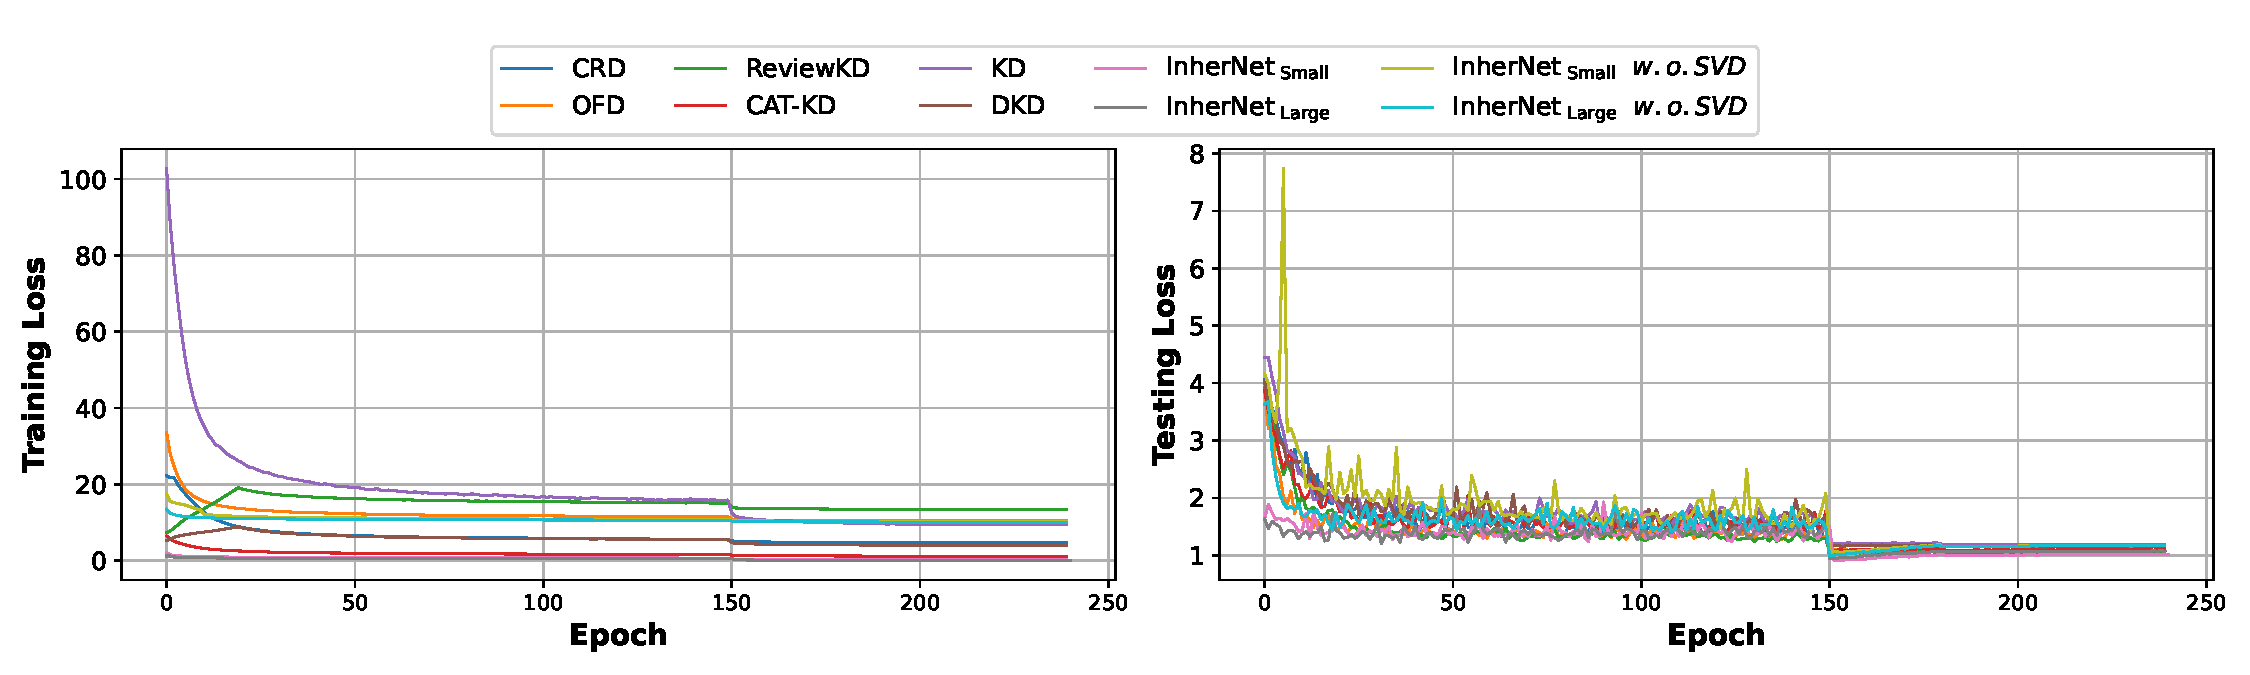
\includegraphics[width=0.7\linewidth]{figures/loss.pdf}
%     \vspace{-0.3cm}
%     \textbf{\caption{The training and testing loss curves of InherNet and various KD methods during training.}
%     \label{fig:loss}}
%     % \vspace{-0.5cm}
% \end{figure*}



\subsection{Language: GLUE Benchmark}
\label{sec:language}
% - 语言任务（Language Model with T5）

% \subsubsection{Settings}
In this task, we evaluate InherNet's performance on multiple text tasks. The experimental setup is as follows:

\textbf{Datasets.} To remain consistent with prior research~\citep{raffel2019exploring}, we train and evaluate InherNet's performance on the GLUE benchmark~\citep{wang2018glue}.

% \footnote{Following prior work~\citep{raffel2019exploring, devlin2019bert}, we do not experiment with the WNLI dataset due to its adversarial nature.}





\textbf{Baselines.} Our experiments are based on the T5 model~\citep{raffel2019exploring} implemented in HuggingFace~\citep{wolf-etal2020transformers}. Due to the lack of widely known and reproducible T5-based KD methods, we use the traditional KD method~\citep{hinton2015distilling}, with a teacher-student setup of T5-Base/T5-Small with parameters 222M/60M.

Beyond the T5 experiments, we also apply InherNet to a larger decoder-only LM, LLaMA-2-7B~\cite{raffel2019exploring,touvron2023llama}. For such autoregressive LMs, conventional token-level KD is difficult to deploy due to the $32$K-dimensional vocabulary softmax, strict teacher-forcing requirements, and tokenizer mismatches between teacher and student, so we do not include standard KD baselines here. Instead, we compare a self-distilled LLaMA-2-7B baseline (teacher and student sharing the same weights, offering no compression) with an InherNet model constructed from the same teacher. As detailed in Appendix~\ref{app:inhernet-llama}, the resulting $4.2$B-parameter model slightly outperforms the $7$B teacher on GSM8K while maintaining competitive performance on MMLU-style evaluations, indicating that our inheritance mechanism scales to large Transformer LMs without relying on KD.


% \textbf{Experimental Details.} We use the AdamW optimizer~\citep{loshchilov2017decoupled} with a training learning rate of 0.0003 and a distillation learning rate of 0.0005, with weight decay set to 0.1. The number of training epochs is 10, the batch size is 32, and the distillation coefficient and temperature are set to 0.3 and 4.0, respectively. The rank and number of expert heads of InherNet are set to 128 and 2, respectively, with a total of 128M parameters.

% 在本任务中，我们评估了InherNet在多个文本任务上的表现，实验设置如下：

% 数据集
% 为了与之前的研究一致~\citep{raffel2019exploring}，我们在GLUE基准~\citep{wang2018glue}上训练和评估InherNet的性能。该基准包含多个任务：释义检测（MRPC, QQP）、情感分类（SST-2）、自然语言推理（MNLI, RTE, QNLI）和语言可接受性（CoLA）~\footnote{遵循之前工作~\citep{raffel2019exploring, devlin2019bert}的做法，由于WNLI数据集具有对抗性，我们未对WNLI进行实验。}。由于原始测试集并未公开，我们在GLUE的验证集上进行了测试。

% 基准模型
% 我们的实验基于HuggingFace实现~\citep{wolf-etal2020transformers}的T5模型~\citep{raffel2019exploring}。由于缺乏广为人知且可复现的基于T5的KD方法，我们采用传统的知识蒸馏（KD）方法~\citep{hinton2015distilling}，教师-学生设置为T5-Small/T5-Base。我们还实现了一个基于T5的简易KD框架，并已在匿名仓库中公开。

% 实验细节
% 由于缺乏相关文献可供参考，我们统一设置了实验参数。我们使用AdamW优化器~\citep{loshchilov2017decoupled}带着训练学习率和蒸馏学习率分别为0.0003和0.0005，权重衰减为0.1。训练轮数设为10，批次大小为32，蒸馏系数和温度分别设置为0.3和4.0。

% 在该任务中，我们评估InherNet在多个文本任务上的表现，实验设置如下：
% - Datasets
% % 遵循之前的研究~\citep{raffel2019exploring}，我们在GLUE基准~\citep{wang2018glue}上训练和评估InherNet的性能。该基准包括多个functions：释义检测 (MRPC, QQP)、情感分类 (SST-2)、自然语言推理 (MNLI, RTE, QNLI) 和语言可接受性 (CoLA)\footnote{遵循之前的工作~\citep{raffel2019exploring, devlin2019bert}的常见做法，由于WNLI数据集在训练集方面具有对抗性，我们不对WNLI进行实验。}。由于原始测试集并不公开，所以我们在GLUD的验证集上进行测试。
% - Baselines
% 我们的实验基于HuggingFace实现~\citep{wolf-etal2020transformers}的T5模型~\citep{raffel2019exploring}。然而目前缺乏基于T5模型广为人知且可复现的KD方法，因此我们的方法基于传统的KD方法~\citep{hinton2015distilling}，教师-学生设置为T5-Small/T5-Base。我们自己实现了一个简单基于T5的KD框架，其公开在提供的匿名仓库中。

% - 实验细节
% 由于缺乏可参考的solid相关文献，我们在该任务中统一设置实验参数。我们采用AdamW优化器~\citep{loshchilov2017decoupled}，带着训练学习率和蒸馏学习率分别为0.0003和0.0005，权重衰减为 0.1。epoch设置为10，批次大小设置为32。蒸馏系数和温度分别设置为0.3和4.0。

% \subsubsection{Performance}

Table~\ref{tab:glue} shows the performance of InherNet and the distillation method on GLUE tasks. As shown in the table, there is still a performance gap between the distilled student network and the teacher network. However, the InherNet method we proposed narrows this gap through explicit inheritance, which distinguishes it from the traditional implicit learning approach used in KD.
% 表~\ref{tab:glue}展示了InherNet与蒸馏方法在GLUE任务上的表现。由表中可以看出，蒸馏后的学生网络与教师网络之间仍然存在性能差距，而我们提出的InherNet方法，通过显式继承的方式，缩小了这一差距，区别于KD这种传统的隐式学习方式。
% 表~\ref{tab:glue}呈现了InherNet和蒸馏方法在GLUE任务上的性能，从表中我们可以看出蒸馏后的学生网络和教师网络之间仍然存在的一致的性能差距，而我们提出的InherNet这种并非KD这种隐式学习而是显示继承的方法拉近了这种差距。


% Please add the following required packages to your document preamble:
% \usepackage{booktabs}
% \usepackage{graphicx}
\begin{table*}[t]
\centering
\caption{The performance (\%) of InherNet and the distillation method on GLUE tasks. For MRPC, QQP, SST-2, MNLI, RTE, and QNLI, we report Accuracy. For CoLA, we report the Matthews correlation coefficient. For STS-B, we report Pearson and Spearman correlation coefficients.}
\label{tab:glue}
\vspace{-0.3cm}
% \setlength{\tabcolsep}{4.2mm}
\resizebox{0.85\columnwidth}{!}{
\begin{tabular}{@{}c|cccccccc@{}}
\toprule[1.2pt]
Method      & MRPC  & QQP   & SST-2 & MNLI  & RTE   & QNLI  & COLA  & STS-B       \\ \midrule
T5-Base     & 89.21 & 86.54 & 90.71 & 54.93 & 77.98 & 90.13 & 57.00 & 89.04 / 88.88 \\ \midrule
T5-Small    & \underline{88.38} & 81.05 & 87.78 & 53.67 & 72.71 & 87.97 & 48.12 & 85.55 / \underline{86.50} \\
T5-Small+KD & 88.23 & \textbf{84.92} & 89.01 & 53.81 & \textbf{74.31} & \underline{88.76} & \underline{49.31} & \textbf{88.05} / \textbf{87.85} \\ \midrule
InherNet    & \textbf{88.74} & 84.69 & \textbf{89.07} & \textbf{56.34} & \underline{72.93} & \textbf{90.29} & \textbf{50.63} & \underline{86.70} / 86.36 \\ \bottomrule[1.2pt]
\end{tabular}%
}

\vspace{-0.3cm}
\end{table*}




\subsection{Vision $\Leftrightarrow$ Language: Multi-modal Evaluation}
\label{sec:vision-language}
% - 视觉-语言任务（Vision-language Model with CLIP，Image-Text Tasks）
% Image-Text Tasks with CLIP



% \subsubsection{Settings}

In this task, we validate the effectiveness of InherNet in multimodal scenarios and compare it with the recent CLIP-KD~\citep{yang2024clip}. The experimental setup is as follows:

\textbf{Dataset.} We use Conceptual Captions 3M (CC3M)~\citep{sharma2018conceptual} for visual-language pretraining. Additionally, we use the ImageNet validation set for zero-shot classification, with the evaluation protocol consistent with CLIP-related works~\citep{wei2022icar, li2023scaling}.

\textbf{Baselines.} In this task, ResNet-101 serves as the teacher network, while ResNet-18~\citep{he2016deep}, EfficientNet-B0~\citep{tan2019efficientnet} and MobileNetV3~\citep{howard2019searching} are used as students.

% \textbf{Implementation Details.} This experiment follows the setup of CLIP-KD, with all experimental parameters matching theirs. The default settings for InherNet are: a visual encoder rank of 32, a text encoder rank of 64, and 2 expert heads. Retrieval performance is measured by Recall@K (R@K), and other training details can be found in the supplementary material.


% 我们在本任务中验证了InherNet在多模态场景下的有效性，实验设置如下：

% - 数据集
% 由于计算资源限制，我们采用Conceptual Captions 3M (CC3M)~\citep{sharma2018conceptual}进行视觉与语言预训练。CC3M验证集包含13K图像-文本对，用于跨模态检索评估。此外，我们还使用了ImageNet (IN)验证集进行零样本分类，评估协议与CLIP相关工作~\citep{wei2022icar, li2023scaling}一致。

% - 基准
% 表~\ref{tab:conf}展示了多模态评估中使用的视觉和文本编码器配置。ResNet-101作为教师网络，InherNet的默认设置为视觉编码器的rank=32，文本编码器rank=64，专家头数量为2。

% 实现细节
% 本实验遵循CLIP-KD~\citep{yang2024clip}的设置，所有实验参数与其一致，采用Recall@K (R@K)衡量检索性能，其他训练细节见补充材料。

% - 我们在这个任务中检验提出的InherNet在多模态场景下的有效性，实验设置如下：

% - 数据集
% 由于有限的计算资源，我们使用Conceptual Captions 3M (CC3M)~\citep{sharma2018conceptual}进行视觉和语言预训练。其中CC3M 验证集，包括 13K 图像-文本对，用于跨模态检索评估。另外我们使用ImageNet (IN) 验证集用于零样本分类，并遵循与CLIP相关工作~\citep{wei2022icar, li2023scaling}一致的评估协议。

% - baselines。如表~\ref{tab:conf}所示展示了在多模态评估中使用的视觉和文本编码器的配置，其中ResNet-101作为教师网络，InherNet默认设置visual encoder的rank为32，text encoder的rank为64，专家头的数量为2。

% - 实现细节
% 我们follow CLIP-KD~\citep{yang2024clip}的实验设置，实验的参数设置跟其保持一致，采用 Recall@K (R@K) 来衡量在K个最近邻居中的检索性能，其他训练设置在补充材料中。
% 我们采用AdamW优化器，带着学习率为0.001，权重衰减为 0.1。应用余弦学习率调度，在 30 个 epoch 内线性预热 10K 次迭代。 批次大小设置为1024，对于CLIP-KD的超参数设置与原论文~\citep{yang2024clip}一致，其他训练设置遵循原始CLIP~\citep{radford2021learning}。值得注意的是，由于有限的计算资源，我们的实验仅在CC3M进行预训练，其他实验设置与CLIP-KD原论文保持一致。遵循标准设置，我们采用 Recall@K (R@K) 来衡量在K个最近邻居中的检索性能。




% % Please add the following required packages to your document preamble:
% % \usepackage{booktabs}
% % \usepackage{multirow}
% % \usepackage{graphicx}
% \begin{table}[t]
% \centering
% \setlength{\tabcolsep}{1mm}
% \begin{tabular}{@{}cc|cccc@{}}
% \toprule[1.2pt]
% \multicolumn{2}{c|}{Visual encoder: CNN}                           & \multicolumn{4}{c}{Text encoder: Transformer}                                                                                                            \\ \midrule
% \multicolumn{1}{c|}{Model}           & \multicolumn{1}{l|}{Params} & \multicolumn{1}{c|}{Layer}               & \multicolumn{1}{c|}{Width}                & \multicolumn{1}{c|}{Head}               & Params                  \\ \midrule
% \multicolumn{1}{c|}{ResNet-101}      & 56.26M                      & \multicolumn{1}{c|}{12}                  & \multicolumn{1}{c|}{512}                  & \multicolumn{1}{c|}{8}                  & 37.83M                  \\ \midrule
% \multicolumn{1}{c|}{ResNet-18}       & 11.43M                      & \multicolumn{1}{c|}{\multirow{3}{*}{12}} & \multicolumn{1}{c|}{\multirow{3}{*}{384}} & \multicolumn{1}{c|}{\multirow{3}{*}{6}} & \multirow{3}{*}{21.29M} \\
% \multicolumn{1}{c|}{EfficientNet-B0} & 4.66M                       & \multicolumn{1}{c|}{}                    & \multicolumn{1}{c|}{}                     & \multicolumn{1}{c|}{}                   &                         \\
% \multicolumn{1}{c|}{MobileNetV3}     & 2.04M                       & \multicolumn{1}{c|}{}                    & \multicolumn{1}{c|}{}                     & \multicolumn{1}{c|}{}                   &                         \\ \midrule
% \multicolumn{1}{c|}{InherNet}        & 12.74M                      & \multicolumn{1}{c|}{12}                  & \multicolumn{1}{c|}{512}                  & \multicolumn{1}{c|}{8}                  & 18.95M                  \\ \bottomrule[1.2pt]
% \end{tabular}%
% \vspace{-0.2cm}
% \caption{Configuration of paired visual and text encoders used in multimodal evaluation.}
% \label{tab:conf}
% \vspace{-0.3cm}
% \end{table}

% \subsubsection{Performance}


Table~\ref{tab:cross_model} shows the cross-modal retrieval performance on the CC3M validation set and zero-shot classification performance on ImageNet validation set for InherNet and its student network distilled through CLIP-KD trained on the CC3M dataset. The proposed InherNet generally outperforms other baseline methods in various multimodal tasks, with its performance consistently significantly higher than that of the teacher network, further validating the effectiveness of InherNet in multimodal scenarios.
% 表~\ref{tab:cross_model}展示了在CC3M数据集上训练的InherNet及其通过CLIP-KD蒸馏的学生网络，在CC3M验证集上的跨模态检索性能和零样本ImageNet分类性能。我们观察到，蒸馏后的EfficientNet-B0模型性能始终优于教师网络，这可能是因为在训练样本不足时，教师网络容易出现参数冗余，而学生网络能够更充分地进行学习。此外，提出的InherNet在不同的多模态任务中普遍优于其他基准方法，且其性能 consistently 显著高于教师网络，进一步验证了在多模态场景中InherNet的有效性。

% 表~\ref{tab:cross_model}报告了在CC3M训练的InherNet和带着CLIP-KD蒸馏的学生网络在CC3M验证集的跨模态检索和零样本ImageNet分类的性能。我们注意到蒸馏的EfficientNet-B0一致超过教师网络，这可能是由于当训练样本数不够时，教师网络容易参数冗余，而学生网络更能充分学习，而提出的InherNet在不同的多模态任务中普遍优于其他baselines，且一致显著高于教师网络，表明InherNet的有效性。







% % % \noindent
% \begin{figure}[t]
%     \centering
%     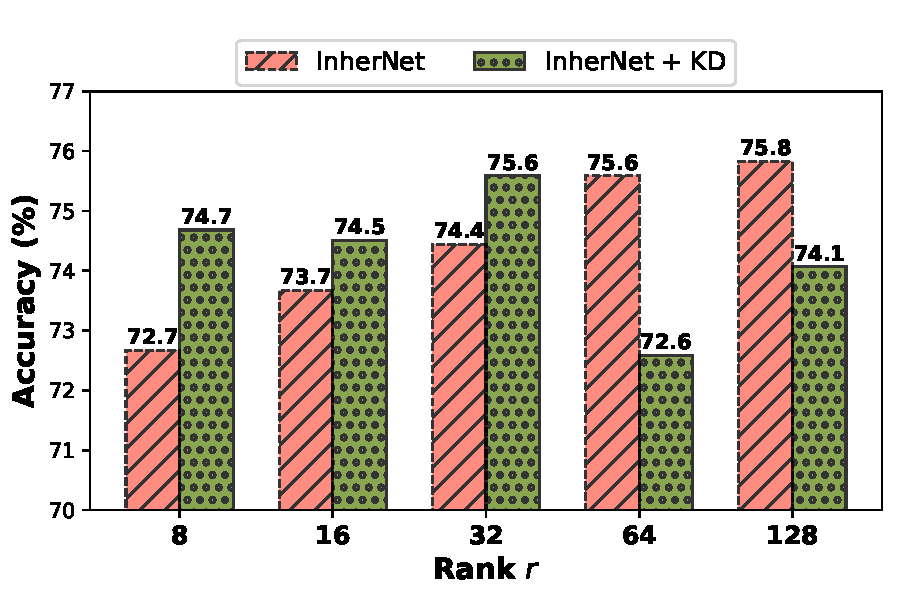
\includegraphics[width=0.8\linewidth]{figures/inhernet_kd_.pdf}
%     \vspace{-0.3cm}
%     \textbf{\caption{\small The impact of distillation on InherNet of different scales with varying ranks.}
%     \label{fig:inhernet_kd}}
%     % \vspace{-0.5cm}
% \end{figure}


% \begin{figure}[t]
%     \centering
%     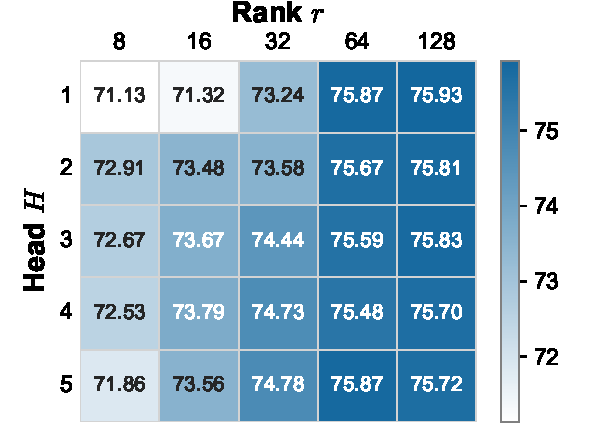
\includegraphics[width=0.8\linewidth]{figures/rank_head.pdf}
%     \vspace{-0.3cm}
%     \textbf{\caption{\small The impact of rank size $r$ and the number of expert heads $H$ on the performance of the  proposed InherNet.}
%     \label{fig:rank_head}}
%     % \vspace{-0.5cm}
% \end{figure}





% \begin{figure}
% %     % \vspace{-0.1cm}
%     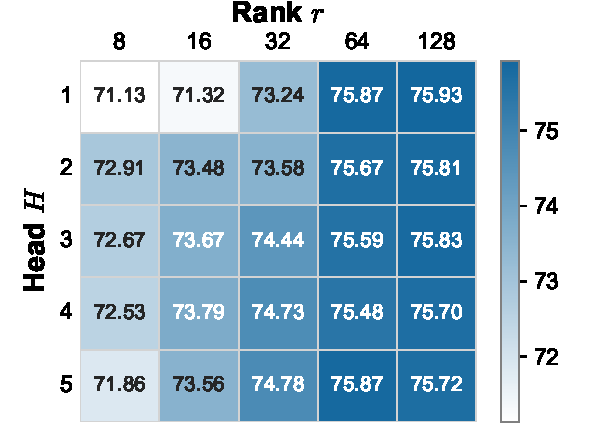
\includegraphics[width=0.7\linewidth]{figures/rank_head.pdf}
%     \vspace{-0.45cm}
%     \textbf{\caption{The impact of rank size $r$ and the number of expert heads $H$ on the performance of the  proposed InherNet.}
%     \label{fig:rank_head}}
%     % \vspace{-0.5cm}
% \end{figure}

% Please add the following required packages to your document preamble:
% \usepackage{booktabs}
% \usepackage{multirow}
% \usepackage{graphicx}
\begin{table*}[t]
\centering
\caption{Comparison of cross-modal retrieval on the CC3M validation set and zero-shot classification on ImageNet validation set performance (\%) between InherNet and the student networks distilled with CLIP-KD trained on CC3M dataset.}
\label{tab:cross_model}
\vspace{-0.3cm}
% \setlength{\tabcolsep}{4.7mm}
\resizebox{0.75\columnwidth}{!}{
\begin{tabular}{@{}c|ccc|ccc|cc@{}}
\toprule[1.2pt]
\multirow{2}{*}{Method} & \multicolumn{3}{c|}{I2T} & \multicolumn{3}{c|}{T2I} & \multicolumn{2}{c}{Classification} \\ \cmidrule(l){2-9} 
                        & R@1    & R@5    & R@10   & R@1    & R@5    & R@10   & top-1        & top-5       \\ \midrule
ResNet-101              & 30.58  & 53.95  & 63.49  & 29.31  & 54.13  & 63.31  & 15.70            & 32.75           \\ \midrule
ResNet-18               & 31.03  & 56.41  & 65.82  & 30.78  & 55.74  & 65.35  & 15.93            & 33.83           \\
EfficientNet-B0         & \textbf{33.65}  & \textbf{58.72}  & \textbf{68.28}  & \underline{32.65}  & \underline{58.21}  & \underline{67.92}  & \underline{17.30}            & \underline{35.75}           \\
MobileNetV3             & 29.07  & 53.43  & 63.59  & 28.10  & 53.11  & 63.35  & 14.59            & 31.68           \\ \midrule
InherNet                & \underline{32.17}  & \underline{57.17}  & \underline{67.82}  & \textbf{33.01}  & \textbf{59.88}  & \textbf{68.72}  & \textbf{17.39}            & \textbf{36.65}           \\ \bottomrule[1.2pt]
\end{tabular}%
}

\vspace{-0.5cm}
\end{table*}






\subsection{Insights on InherNet}
\label{sec:observation}


Based on the image classification task, we conduct analytical experiments under the teacher-student setup of ResNet56/ResNet20. We provide experimental details and results for all insights in Appendix~\ref{sec:observations}. The observed insights are as follows.

% 基于图像分类任务，我们在ResNet56/ResNet20的教师/学生设置，一种常见的设置中进行分析实验，观察结果如下。
% 观察1：蒸馏继承网络有时并不一定能带来更好的收益，特别是小的继承模型蒸馏往往带来正收益，而大的继承网络蒸馏往往带来负收益，未来探索其他KD的效果
% 观察2：继承网络很多情况下甚至超过教师网络，这跟提出的MoE方法有关（对应理论分析部分），此外探索增加rank，以及增加专家头的关系并跟教师网络比较
% 观察3：跟KD方法相比，提出的InherNet收敛要更快。
% - KD往往能给小的继承网络带来性能收益，而有损大的继承网络的性能
% - Rank显著影响模型性能，多个专家头效果比单头更好
% - 相比于传统的蒸馏方法，提出的InherNet的收敛速度显著更快。
% \begin{githubquote}

% \end{githubquote}
\textbf{Insight 1.} \textit{Distillation benefits small-scale InherNet, but harms the performance of large-scale InherNet.} It is aligned with our theory: as the rank $r$ grows, the InherNet $f_r$ converges in function space toward the teacher $f_W$ in Proposition~\ref{prop:knowledge-preservation_}. In the high-rank regime, the task loss alone can drive it to that generalize slightly better than the teacher. In contrast, the KD loss penalizes any deviation from the teacher's logits, acting as an overly strong regularizer. More details are shown in Appendix~\ref{app:distill-large-r}.

% We construct InherNets of different scales based on various ranks ($r = 8, 16, 32, 64, 128$), using them as student networks, and adopt ResNet-56 as the teacher network for knowledge distillation~\citep{hinton2015distilling}. Figure~\ref{fig:inhernet_kd} shows the performance changes of InherNets of different scales before and after distillation. The results indicate that small-scale InherNets ($r \leq 32$) benefit significantly from distillation, with smaller models showing greater improvement. In contrast, large-scale InherNets experience a performance drop after distillation. We speculate that this is because large-scale InherNets already inherit most of the teacher's knowledge and may even outperform the teacher through independent training (as shown in Table~\ref{tab:cifar}, InherNet\textsubscript{\ Large} consistently outperforms the teacher network). Therefore, further distillation offers little benefit to such networks and may even have a negative effect.

% 我们根据不同的rank（$r=8, 16, 32, 64, 128$）构建了不同规模的InherNet，并将其作为学生网络，采用ResNet-56作为教师网络进行知识蒸馏~\citep{hinton2015distilling}。图~\ref{inhernet_kd}展示了蒸馏前后，不同规模InherNet的性能变化。从图中可以看出，小规模的InherNet（$r \leq 32$）在蒸馏后性能有显著提升，且网络规模越小，提升越明显。相比之下，大规模InherNet在蒸馏后反而出现了性能下降。我们推测这是由于大规模InherNet已能充分继承教师网络的知识，其自身训练过程中甚至能够超越教师网络的性能（如图~\ref{fig:cifar}所示，InherNet\textsubscript{Large}几乎在各项指标上全面优于教师网络），因此，此类网络再进行蒸馏已无明显收益，甚至可能适得其反。

% 我们根据rank的不同(r=8,16,32,64和128)设置了不同规模的InherNet，并将其作为学生网络，ResNet56充当教师网络进行蒸馏~\citep{hinton2015distilling}。图~\ref{inhernet_kd}展示了蒸馏前后不同规模的InherNet的性能比较。从图中可以看出，小规模继承网络($r\leq 32$)蒸馏后性能显著提升，且规模越小提升越明显，而蒸馏大规模继承网络有损性能，我们认为这是因为大规模继承网络已经充分继承教师网络知识，后天学习过程甚至超过教师网络（这可以从图~\ref{fig:cifar}中可以看出，InherNet_{Large}几乎全面超过教师网络），即这样的蒸馏失去了价值。

% \begin{githubquote}

% \end{githubquote}
\textbf{Insight 2.} \textit{Rank significantly affects model performance; using multiple expert heads performs better than a single head.}

% We investigate the impact of rank size $r$ and the number of expert heads $H$ on the performance of InherNet. As shown in Figure~\ref{fig:rank_head}, rank exerts a more significant influence on InherNet. We attribute this to the fact that rank directly determines how well InherNet inherits core knowledge from the teacher network, which is crucial for subsequent learning—an advantage that cannot be compensated by simply increasing model parameters such as the number of expert heads. Moreover, we also observe that single-head structures perform worse than multi-head ones. However, increasing the number of heads beyond one ($H > 1$) does not necessarily lead to further gains. We speculate that while multi-head mechanisms combined with gating improve generalization and diversity, too many expert heads may cause overfitting.

% 我们探讨了秩的大小$r$和专家头的数量$H$对InherNet性能的影响。从图~\ref{fig:rank_head}可以看出，秩对InherNet的影响更为显著。我们认为这是因为rank直接决定了InherNet能够继承教师网络核心知识的程度，这对于后续学习至关重要，而这一点并不能通过简单增加模型参数（如增加专家头数量）来弥补。此外，我们还观察到，相较于多头结构，单头结构的效果较差；然而，当采用多头结构（即 head $H > 1$）时，继续增加头的数量并不一定带来性能提升。我们推测，这可能是因为多头机制结合门控策略有助于提升模型的泛化能力和多样性，而专家头数量过多反而可能导致模型过拟合。

% 我们探索了rank $r$和专家头$H$对继承网络性能的影响，从图~\ref{fig:rank_head}中可以看出，rank对InherNet的影响更大，我们认为这是因为rank直接决定了InherNet继承教师网络主要知识的多少，这对于后天的学习至关重要，而并非增加参数（专家头的数量）所能弥补。此外我们也发现单头效果不如多头好，而多个头（head $h>1$）时增加头个数不一定使模型性能受益，我们将其归因于多头以及门控机制使模型更加泛化多样，而过多的专家头容易使模型过拟合。


% \begin{githubquote}

% \end{githubquote}
\textbf{Insight 3.} \textit{Compared to traditional distillation methods, InherNet converges significantly faster.}

% We select the commonly used KD method with epoch=240 from Sec.~\ref{sec:result_cifar} as the subject for studying model convergence speed. Figure~\ref{fig:loss} shows the change in training and testing loss during the training process for different methods in a single experiment. The results indicate that InherNet converges significantly faster than traditional KD methods. However, InherNet without SVD initialization shows highly unstable generalization performance during training. This phenomenon strongly supports the effectiveness of the proposed extended SVD method in accelerating model convergence and further confirms the correctness of the theoretical analysis in Sec.~\ref{sec:convergence} and Sec.~\ref{sec:parameter}.

% 我们选取了Sec.~\ref{sec:result_cifar}中常见且epoch=240的KD方法，作为研究模型收敛速度的对象。图~\ref{fig:loss}展示了不同方法在一次实验中训练与测试损失随训练过程的变化曲线。结果表明，InherNet收敛速度显著快于传统KD方法；而未经过SVD初始化的InherNet在训练过程中泛化性能极不稳定性，这一现象有力验证了所提出的扩展SVD方法在加速模型收敛方面的显著优势，并进一步印证了Sec.\ref{sec:convergence}与Sec.\ref{sec:parameter}中相关理论分析的正确性。
% 我们选择在Sec.~\ref{sec:result_cifar}中常见的且epoch一致的KD方法用于研究收敛速度，图~\ref{fig:loss}展示了在一次实验中不同方法的训练和测试loss曲线的变化。我们发现，InherNet的很快收敛，跟传统知识蒸馏相比更加显著，而没有经过SVD初始化的InherNet在训练时泛化性能极端不稳定，这有力证实了提出的扩展SVD在加速收敛方面的显著优势并进一步证实了Sec.~\ref{sec:convergence}和Sec.~\ref{sec:parameter}中理论分析的正确性。

\subsection{Ablation Study}
\label{sec:ablation}
% Please add the following required packages to your document preamble:
% \usepackage{booktabs}
% \usepackage{graphicx}
% \begin{table}[t]
% \centering
% \setlength{\tabcolsep}{0.5mm}
% \begin{tabular}{@{}c|cccc@{}}
% \toprule[1.1pt]
% Variants  & ResNet32$\times$4 &  WRN-40-2 & ResNet56 & ResNet110 \\ \midrule
% w.o. svd  & 76.68         & 75.42    & 69.35    & 74.13     \\
% w.o. gate & 78.17          & 76.08    & 73.22    & 75.64     \\
% w. sym.    & 77.92         & 75.98    & 73.28    & 75.45     \\ \midrule
% InherNet  & \textbf{78.53}             & \textbf{76.39}    & \textbf{73.67}    & \textbf{75.88}     \\ \bottomrule[1.1pt]
% \end{tabular}%
% \vspace{-0.2cm}
% \caption{Ablation study of different variants on InherNet.}
% \label{tab:ablation}
% \vspace{-0.4cm}
% \end{table}


\begin{wraptable}{r}{0.6\textwidth} % 'r' 代表表格在右侧, 'l' 代表在左侧。 '0.5\textwidth' 是表格的宽度，您可以根据需要调整。
    % \vspace{-0.1cm} % 调整与上方文本的垂直间距
    \centering
    \caption{Ablation study of different variants on InherNet.}
    \label{tab:ablation}
    \vspace{-0.3cm}
    % \setlength{\tabcolsep}{0.5mm}
    \resizebox{0.55\columnwidth}{!}{
    \begin{tabular}{@{}c|cccc@{}}
    \toprule[1.1pt]
    Variants  & ResNet32$\times$4 &  WRN-40-2 & ResNet56 & ResNet110 \\ \midrule
    w.o. svd  & 76.68           & 75.42     & 69.35    & 74.13     \\
    w.o. gate & 78.17           & 76.08     & 73.22    & 75.64     \\
    w. sym.   & 77.92           & 75.98     & 73.28    & 75.45     \\ \midrule
    InherNet  & \textbf{78.53}  & \textbf{76.39}  & \textbf{73.67}  & \textbf{75.88}  \\ \bottomrule[1.1pt]
    \end{tabular}%
    }
    \vspace{-0.4cm} % 调整与下方文本的垂直间距
\end{wraptable}

We construct three variants of InherNet$_{\ \text{Large}}$ with the teacher network ResNet56 on CIFAR-100 to investigate the critical roles of different components. Specifically, ``w.o. svd'' denotes the absence of SVD initialization, "w.o. gate" removes the gating mechanism, and "w. sym." adopts a symmetric structure (with two branches and two expert heads, similar to LoRA+MoE~\citep{liu2024moemeetsllmsparameter}). The experimental results are shown in Table~\ref{tab:ablation}, from which we observe the following: (1) SVD initialization contributes the most to performance improvement. This is not only because it allows the network to inherit a substantial amount of beneficial knowledge from the teacher network, but also because it stabilizes training, accelerates convergence, and helps the model find the optimal solution more quickly and accurately, as illustrated in Insight 3 of Sec.~\ref{sec:observation}. (2) The gating mechanism enables effective dynamic routing in most cases, and it is especially crucial for lightweight inherited networks. (3) Under the same parameter size, the symmetric architecture underperforms compared to asymmetric ones. This is because the asymmetric architecture introduces a structural inductive bias~\citep{parton2020mixtures}, which enhances the diversity among experts.

% 我们在CIFAR-100上构建了三种InherNet$_{\ \text{Large}}$变体，以探讨不同组件的关键作用。其中，"w.o. svd"表示未使用SVD初始化，"w.o. gate"表示移除门控机制，"w. sym"表示采用对称结构（主干分支与专家头的数量均为2）。实验结果如表~\ref{tab:ablation}所示，由表中可以发现：

% (1) SVD初始化对性能提升最显著，这不仅因为 SVD 初始化能较好地继承教师网络的大量有益知识，还能稳定训练过程、加快收敛，并更快、更准确地找到最优解，如Sec.~\ref{sec:observation}的观察3所诠释。
% (2) 门控机制在多数场景下能实现有效的动态路由，特别是在参数规模较小的继承网络中尤为关键。
% (3) 在参数量相同的条件下，对称结构表现不如非对称结构，因为非对称结构引入了结构性归纳偏置~\citep{parton2020mixtures}，有助于增强专家间的差异性。


% 我们通过在CIFAR-100上正对不同的教师网络构建三种不同的InherNet$_{\ \text{Large}}$变体以探讨不同组件的关键影响。"w.o. svd"表示InherNet没有SVD初始化，"w.o. gate"指移除门控机制，"w. sym"指的是InherNet采用对称结构(即主干分支和专家头数都设置为2)，结果如表~\ref{tab:ablation}所示，从表中可以看出：(1) SVD初始化对模型性能影响最大，这是因为SVD初始化不仅仅继承教师网络的绝大部分有益知识，根据Sec.~\ref{sec:observation}中的观察3还能够稳定模型训练，加速收敛的同时更快更好找到最优解。(2) 门控机制在大部分情况下都能发挥动态路由的作用，特别适用于参数规模较小的继承网络。(3) 在同等参数量的条件下，对称结构不如非对称结构，这是因为非对称结构本身引入了结构上的归纳偏置~\citep{parton2020mixtures}，使不同专家更容易区分.

% - 没有SVD初始化
% - 没有路由机制
% - 在相同参数的情况下，非对称和对称结构的比较

\vspace{-0.2cm}
\section{Related Work}
% \label{sec:related_work}
% - 知识蒸馏
We summarize previous research of knowledge distillation (KD)~\citep{hinton2015distilling} and low-rank decomposition~\citep{denton2014exploiting}; extensive discussion and comprehensive comparisons appear in Appendix~\ref{sec:related_work}.

% - 低秩分解

% 然而这些方法仅仅在视觉任务上而并没有扩展到其他模态任务上
% \subsection{Knowledge Distillation}
% Knowledge distillation (KD)~\citep{hinton2015distilling} is an efficient model compression technique that helps a smaller student network learn better during training by transferring the knowledge of a larger teacher network. Traditional knowledge distillation methods typically focus on minimizing the prediction differences between the teacher and student networks, typically using loss functions like KL divergence calculated from the teacher's logit outputs. ecent research has focused on two main directions: logit distillation~\citep{hinton2015distilling, chen2020online, li2020online, li2022curriculum, zhao2022decoupled, jin2023multi, zhang2023blindly, sun2024logit} and feature distillation~\citep{yim2017gift, peng2019correlation, heo2019comprehensive, chen2021distilling, li2021online, chen2022knowledge, lin2022knowledge, guo2023class}. In logit distillation, the goal is to optimize the similarity of the outputs by matching the prediction probabilities of the teacher and the student, while feature distillation focuses on transferring the intermediate feature representation within the model, providing more fine-grained learning information. However, due to the limited capacity of the student network, especially the performance ceiling imposed by the teacher network, the student's performance often struggles to match that of the teacher~\citep{gou2021knowledge, hu2023teacher, xu2024survey}.


% % 知识蒸馏~\citep{hinton2015distilling}是一种高效的模型压缩技术，它通过将大型教师网络的知识迁移到较小的学生网络，帮助后者在训练过程中更好地学习。传统的知识蒸馏方法通常侧重于最小化教师与学生网络预测之间的差异，常用的损失函数如KL散度，通常是通过教师网络的logit输出计算的。近年来，相关研究主要集中在logit蒸馏~\citep{hinton2015distilling, chen2020online, li2020online, li2022curriculum, zhao2022decoupled, jin2023multi, zhang2023blindly, sun2024logit}和特征蒸馏~\citep{yim2017gift, peng2019correlation, heo2019comprehensive, chen2021distilling, li2021online, chen2022knowledge, lin2022knowledge, guo2023class}两大方向。在logit蒸馏中，目标是通过匹配教师和学生的预测概率来优化输出的相似性，而特征蒸馏则专注于传递模型内部的中间表示特征，提供更为细粒度的学习信息。然而，由于学生网络容量的限制，尤其是教师网络性能上限的影响，学生网络的性能往往难以达到教师网络的水平~\citep{gou2021knowledge, hu2023teacher, xu2024survey}。


% % 知识蒸馏~\citep{hinton2015distilling}是一种有效的模型压缩方法，通过将大型教师网络的知识转移到较小的学生网络中，帮助学生网络在训练过程中更好地学习。传统的知识蒸馏方法通常基于最小化教师与学生网络预测之间的差异，常见的损失函数如KL散度，通常通过教师网络的logit输出计算。近年来的相关研究集中在logit蒸馏~\citep{hinton2015distilling, chen2020online, li2020online, li2022curriculum, zhao2022decoupled, jin2023multi, zhang2023blindly, sun2024logit}和特征蒸馏~\citep{yim2017gift, peng2019correlation, heo2019comprehensive, chen2021distilling, li2021online, chen2022knowledge, lin2022knowledge, guo2023class}两大方向发展，其中，logit蒸馏通过匹配教师和学生的预测概率来优化输出的相似性，而特征蒸馏则专注于转移模型内部的中间表示特征，通常能获得更为细粒度的学习信息。

% \subsection{Low-Rank Decomposition}

% In recent years, low-rank decomposition has become a key focus in model compression, aiming to reduce storage requirements and improve inference efficiency by approximating weight matrices through the product of low-rank matrices. Initially applied to the weight matrices in convolutional neural networks (CNNs), particularly the 4D tensors of convolutional kernels, early studies~\citep{denton2014exploiting, lebedev2014speeding, tai2015convolutional, xu2019trained, yang2020learning} focused on effective matrix and tensor decomposition methods, such as using CP decomposition to decompose convolutional kernels into multiple low-rank layers~\citep{lebedev2014speeding}. While this approach reduces model complexity, it can lead to issues like vanishing or exploding gradients when scaling to large, deep networks, making training and fine-tuning more challenging~\citep{tai2015convolutional}. To address this, subsequent research has reshaped high-dimensional tensors into 2D matrices and applied techniques like singular value decomposition (SVD) for compression, effectively reducing computational load. For example, channel decomposition~\citep{zhang2015accelerating} using SVD reduces convolution layers to two, with one layer being a $1\times 1$ convolution, and further eliminates small singular value channels to reduce computation. However, these low-rank decomposition methods are typically applicable to specific CNN structures and vision tasks. Moreover, existing methods have not explored the potential link with student networks in KD, while our proposed InherNet aims to establish an effective bridge between the two.

% In recent years, low-rank decomposition techniques have become an important research direction in the field of model compression. The core idea is to approximate the weight matrix through the product of low-rank matrices, thereby reducing the model's storage requirements and improving inference efficiency. This technique was initially applied to the weight matrices in Convolutional Neural Networks (CNNs), particularly the 4D tensor of convolutional kernels. Early studies~\citep{denton2014exploiting, lebedev2014speeding, tai2015convolutional, xu2019trained, yang2020learning} focused on designing efficient matrix and tensor decomposition methods, especially by cascading low-rank layers to approximate the convolutional layer computations of pre-trained networks, such as using CP decomposition to decompose convolutional kernels into multiple low-rank convolutional layers~\citep{lebedev2014speeding}. Although this approach has advantages in reducing model complexity, it can lead to an increased number of network layers when dealing with large-scale and deep networks, which may cause vanishing or exploding gradients, making training and fine-tuning difficult~\citep{tai2015convolutional}. To address this issue, subsequent studies have proposed reshaping high-dimensional tensors into 2D matrices and applying techniques such as Singular Value Decomposition (SVD) for compression to achieve low-rank approximation. These methods decompose convolutional kernels into multiple successive layers, effectively reducing computational load. For example, the channel decomposition method~\citep{zhang2015accelerating} uses SVD to decompose a convolutional layer into two layers, one of which is a $1 \times 1$ convolution layer, further reducing computational complexity by removing channels with smaller singular values. This method leverages channel redundancy and reduces training parameters, thereby improving computational efficiency. However, these low-rank decomposition methods are typically applicable to specific CNN structures and vision tasks, whereas the Neural Network Inheritance (NII) we propose is more versatile. Furthermore, existing methods have not explored the potential connection with the student network in Knowledge Distillation (KD), while our proposed InherNet aims to establish an effective communication bridge between the two.
% 近年来，低秩分解技术已成为模型压缩领域的重要研究方向，其核心思想是通过低秩矩阵的乘积近似权重矩阵，从而减少模型存储需求并提升推理效率。该技术最早应用于卷积神经网络（CNN）中的权重矩阵，特别是卷积核的4维张量。早期研究~\citep{denton2014exploiting, lebedev2014speeding, tai2015convolutional, xu2019trained, yang2020learning}集中于设计有效的矩阵和张量分解方法，特别是通过级联低秩层逼近预训练网络的卷积层计算，如利用CP分解将卷积核分解为多个低秩卷积层~\citep{lebedev2014speeding}。尽管这种方法在降低模型复杂度方面具有优势，但在处理大规模和深层网络时，分解后的网络层数增加，容易导致梯度消失或爆炸，从而使训练和微调变得困难~\citep{tai2015convolutional}。为解决这一问题，后续研究提出将高维张量重塑为二维矩阵，并应用奇异值分解（SVD）等技术进行压缩，实现低秩近似。这些方法将卷积核分解为多个连续层，有效减少计算量。例如，通道分解法~\citep{zhang2015accelerating}通过SVD将卷积层分解为两层，其中一层为$1\times 1$卷积层，进一步通过去除较小奇异值的通道减小计算量。该方法利用了通道冗余，减少了训练参数，从而提高了计算效率。然而，这些低秩分解方法通常仅适用于特定CNN结构和视觉任务，而我们提出的神经网络继承（NII）则更具普适性。此外，现有方法未深入探讨与知识蒸馏（KD）中学生网络的潜在联系，而我们提出的InherNet旨在为两者建立有效的沟通桥梁。

% 近年来，低秩分解技术已成为模型压缩领域的重要研究方向。其核心思想是通过低秩矩阵的乘积来逼近权重矩阵，从而减小模型的存储需求并提升推理效率。这一思想最早被应用于卷积神经网络（CNN）的权重矩阵，尤其是卷积核的 4 维张量。早期的工作~\citep{denton2014exploiting, lebedev2014speeding, tai2015convolutional, xu2019trained, yang2020learning}集中于设计有效的矩阵和张量分解方法，特别是利用级联低秩层来逼近预训练网络的卷积层计算，例如通过 CP 分解将卷积核分解为多个连续的低秩卷积层~\citep{lebedev2014speeding}。然而，这种方法虽然在降低模型复杂度方面具有一定优势，但在进行更大规模和更深层网络的分解时，分解后的网络层数增加，容易导致梯度消失或者爆炸，使训练和微调变得困难~\citep{tai2015convolutional}。为了解决这一问题，后续研究提出了将高维张量重塑为二维矩阵，并应用奇异值分解（SVD）等矩阵分解技术来进行压缩，从而实现低秩近似。这些方法将卷积核分解为多个连续层，从而有效减少了计算量。例如，通道分解法~\citep{zhang2015accelerating}利用 SVD 将卷积层分解为两层，其中一层为 $1\times1$ 的卷积层，可以通过去除较小奇异值的通道来进一步减小计算量。这种方法利用了通道冗余，并能够减少网络的训练参数，从而提高了计算效率。然而这些低秩分解方法仅限于特定的CNN结构和视觉任务，我们提出的神经网络继承（NII）与其区分开来。此外，这些方法并没有探究与KD中学生网络的潜在关系，我们提出的InherNet旨在为两者建立一个有效的沟通桥梁。

% 用低秩矩阵的乘积来逼近权重矩阵是压缩 DNN 的一个直接想法。 该领域的早期工作侧重于设计矩阵和张量分解方案，特别是对于卷积核的 4 维张量，以便可以利用级联低秩层紧密逼近预训练网络层的运算 [15, 39, 26, 4, 19]。 张量分解技术，特别是 CP 分解，在早期工作中被用来直接将 4 维卷积核分解成 4 个连续的低秩卷积 [19]。 然而，这种分解技术会显著增加所获得网络的层数，这使得它们难以微调以获得良好的性能，尤其是在分解更大更深的模型时 [29]。 因此，后续工作提出将四维张量重塑为二维矩阵，应用奇异值分解 (SVD) 等矩阵分解技术对矩阵进行分解，最后将其重塑回四维张量以获得两个连续层。 值得注意的是，Zhang 等人 [39] 提出了通道分解法，该方法使用 SVD 将具有核大小 
% w
% ×
% h
%  的卷积层分解为两个连续层，其核大小分别为 
% w
% ×
% h
%  和 
% 1
% ×
% 1
% 。 通过利用通道冗余可以实现计算量减少，例如，去除分解层中奇异值较小的通道。 同样，Jaderberg 等人 [15] 提出将卷积层分解为两个连续层，中间通道更少。 他们进一步利用空间冗余将分解层中卷积核的大小分别减小到 
% 1
% ×
% h
%  和 
% w
% ×
% 1
% 。 这些方法为每一层提供了闭式分解。 如果 SVD 是以满秩进行的，则这些方法保证分解后的层执行与原始层相同的操作。 然而，预训练模型的权重可能并非天生就是低秩的，因此通过去除小的奇异值来进行手动施加的低秩分解，不可避免地会导致随着压缩率的增加而精度损失较高

\vspace{-0.2cm}
\section{Conclusion}
\label{sec:conclusion}
\vspace{-0.1cm}

This paper introduces InherNet, a novel approach beyond student that directly inherits both the structure and knowledge of teacher networks. By applying low-rank approximation and leveraging singular value decomposition, InherNet efficiently compresses models while maintaining the expressiveness and performance of the teacher network. Our method demonstrates faster convergence compared to traditional student networks and offers a more stable and effective solution for model compression.

\section*{Acknowledgments}
This research was partially supported by grants from the ``Pioneer'' and ``Leading Goose'' R\&D Program of Zhejiang under Grant No. 2025C02022, the National Natural Science Foundation of China (No.62307032), and Shanghai Rising-Star Program (23QA1409000). Additionally, this work was partially supported by the UK Engineering and Physical Sciences Research Council (EPSRC) [EP/W524694/1].

\newpage
\section{Ethics Statement}
This work is guided by the ethical principles outlined in the ICLR Code of Ethics, prioritizing responsible research practices, scientific rigor, and the broader well-being of society. We recognize the global community of stakeholders in machine learning research and aim to ensure our contributions are beneficial to society while minimizing potential risks. Our research adheres to high standards of integrity, transparency, and reproducibility, with methods and results presented honestly and accurately. We have carefully considered the wider implications of our work, addressing potential concerns related to privacy, safety, and fairness, and have consulted with domain experts to mitigate any unintended consequences. All data used in this study has been handled in line with ethical approvals, safeguarding privacy and confidentiality. We are committed to promoting inclusivity, avoiding bias, and ensuring that our findings are both accessible and socially responsible.

\bibliography{iclr2026_conference}
\bibliographystyle{iclr2026_conference}
\newpage
\section{Appendix}
\appendix
% \section{Supplementary Material--Beyond Distillation: SVD-Driven Low-Rank Layer Decomposition for Neural Network Inheritance}
\label{sec: appendix}





We present the following additional information to include and clarify details that could not be fully covered in the main text.
\begin{tcolorbox}[colback=lightpink, colframe=darkred, title=\textbf{Content}]
\begin{itemize}[leftmargin=*]
\item \textbf{\ref{sec:asymmetric}~Fixed Asymmetric Design}
\begin{itemize}
    \item \ref{sec:evidence}~Empirical Evidence
    \item \ref{sec:support}~Theoretical Support
\end{itemize}
\item \textbf{\ref{app:all}~Theoretical Analysis Supplement} 
\begin{itemize}
    \item \ref{app:algo}~Algorithm Overview (Detailed Procedure)
    \item \ref{app:convergence}~Convergence Guarantees
    \item \ref{app:parameter}~Parameter Efficiency
\end{itemize}
\item \textbf{\ref{sec:exp}~Experimental Details}
\begin{itemize}
    \item \ref{sec:implementation}~Implementation Details 
    \item \ref{sec:results}~Results on ImageNet 
    \item \ref{app:inhernet-llama}~Additional Experiments on Large Transformer Language Models 
    \item \ref{sec:observations}~Experimental Details of Insights on InherNet  
\end{itemize}
\item {\textbf{\ref{sec:related_work}~Related Work}
    \begin{itemize}
        \item \ref{sec:kd}~Knowledge Distillation
        \item \ref{sec:lora}~Low-Rank Decomposition
    \end{itemize} }
\item {
\textbf{\ref{sec:LLM}~The Use of Large Language Models}
}

\end{itemize}
\end{tcolorbox}

\section{Fixed Asymmetric Design}
\label{sec:asymmetric}

\subsection{Empirical Evidence}
\label{sec:evidence}

We attempt to invert InherNet into InherNet$^{\circlearrowleft}$ (\textit{i.e.}, multiple single-dimensionality reduction matrices followed by a dimensionality expansion matrix). We compare the performance of InherNet$^{\circlearrowleft}$ and InherNet across various tasks, as shown in Tables~\ref{tab:cifar_inverse}, \ref{tab:glue_inverse}, and~\ref{tab:cross_model_inverse}. From the results, we observe that InherNet$^{\circlearrowleft}$ consistently underperforms compared to InherNet across all tasks. The performance gap is especially pronounced in text-related tasks, which may be attributed to the fact that, in such tasks, the linear layers adapted for inheritance more effectively preserve and replicate the knowledge from the teacher network. In contrast, convolutional neural networks, due to their higher dimensionality and the necessity of reshaping operations, may suffer greater information loss. We plan to explore further optimization strategies for inheriting convolutional neural networks as a direction for future work.

% We attempt to invert InherNet into InherNet$^{\circlearrowleft}$ (\textit{i.e.}, multiple single-dimensionality reduction matrices and a dimensionality expansion matrix). We compare the performance of InherNet$^{\circlearrowleft}$ and InherNet across tasks，如表~\ref{tab:cifar_inverse}、\ref{tab:glue_inverse}和~\ref{tab:cross_model_inverse}所示。从中我们发现：在所有的任务中，InherNet$^{\circlearrowleft}$性能一致劣于InherNet，特别是在文本任务中性能差距越大，这可能是在文本任务中适配的线性层这一基础层更能重复继承教师网络的知识，而卷积神经网络本身维度较多且需要reshape导致信息可能存在较大损失。我们计划对于继承卷积神经网络的持续优化作为未来探索的方向。


\begin{table*}[th!]
\centering
% \setlength{\tabcolsep}{1.2mm}
\caption{Comparison of top-1 Accuracy (\%) on the CIFAR-100 validation set between InherNet$^{\circlearrowleft}$ and InherNet.}
\vspace{-0.3cm}
\resizebox{\columnwidth}{!}{
\begin{tabular}{@{}c|c|ccccccc@{}}
\toprule[1.2pt]
\multirow{4}{*}{Method}     & \multirow{2}{*}{Teacher} & ResNet32$\times 4$ & VGG13 & WRN-40-2 & WRN-40-2 & ResNet56 & ResNet110 & ResNet110 \\
                          &                          & 79.42              & 74.64 & 75.61    & 75.61    & 72.34    & 74.31     & 74.31     \\ \cmidrule(l){2-9} 
                          & \multirow{2}{*}{Student} & ResNet8$\times 4$  & VGG8  & WRN-40-1 & WRN-16-2 & ResNet20 & ResNet32  & ResNet20  \\
                          &                          & 72.50              & 70.36 & 71.98    & 73.26    & 69.06    & 71.14     & 69.06     \\ \midrule
        \multirow{2}{*}{InherNet$^{\circlearrowleft}$} & Small                    & 75.19              & \textbf{75.84} & 74.17    & \textbf{76.53}    & 71.39    & 71.68     & 71.68     \\ \cmidrule(l){2-9} 
                          & Large                    & \textbf{78.79}              & 71.26 & 75.24    & 76.17    & 73.38    & 74.95     & 74.95     \\ \midrule
\multirow{2}{*}{InherNet} & Small                    & \textbf{77.57}              & 75.68 & \textbf{76.04}    & 76.04    & \textbf{72.67}    & \textbf{74.13}     & \textbf{74.13}     \\ \cmidrule(l){2-9} 
                          & Large                    & 78.53              & \textbf{75.16} & \textbf{76.39}    & \textbf{76.39}    & \textbf{73.67}    & \textbf{75.88}     & \textbf{75.88}     \\ \bottomrule[1.2pt]
\end{tabular}%
}
\label{tab:cifar_inverse}
\vspace{-0.2cm}
\end{table*}



\begin{table*}[t]
\centering

\caption{The performance (\%) of InherNet$^{\circlearrowleft}$ and InherNet on GLUE tasks.}
\label{tab:glue_inverse}
\vspace{-0.3cm}
% \setlength{\tabcolsep}{4.2mm}
\resizebox{0.8\columnwidth}{!}{
\begin{tabular}{@{}c|cccccccc@{}}
\toprule[1.2pt]
Method      & MRPC  & QQP   & SST-2 & MNLI  & RTE   & QNLI  & COLA  & STS-B       \\ \midrule
T5-Base     & 89.21 & 86.54 & 90.71 & 54.93 & 77.98 & 90.13 & 57.00 & 89.04 / 88.88 \\ \midrule
InherNet$^{\circlearrowleft}$    & 87.36 & 83.50 & 87.69 & 56.27 & 72.86 & 89.74 & 50.07 & 86.55 / 85.73 \\ \midrule
InherNet    & \textbf{88.74} & \textbf{84.69} & \textbf{89.07} & \textbf{56.34} & \textbf{72.93} & \textbf{90.29} & \textbf{50.63} & \textbf{86.70} / \textbf{86.36} \\ \bottomrule[1.2pt]
\end{tabular}%
}
\vspace{-0.2cm}
\end{table*}


\begin{table*}[t]
\centering
\caption{Comparison of cross-modal retrieval on the CC3M validation set and zero-shot classification on ImageNet validation set performance (\%) between InherNet$^{\circlearrowleft}$ and InherNet.}
\vspace{-0.3cm}
\label{tab:cross_model_inverse}
% \setlength{\tabcolsep}{4.7mm}
\resizebox{0.75\columnwidth}{!}{
\begin{tabular}{@{}c|ccc|ccc|cc@{}}
\toprule[1.2pt]
\multirow{2}{*}{Method} & \multicolumn{3}{c|}{I2T} & \multicolumn{3}{c|}{T2I} & \multicolumn{2}{c}{Classification} \\ \cmidrule(l){2-9} 
                        & R@1    & R@5    & R@10   & R@1    & R@5    & R@10   & top-1        & top-5       \\ \midrule
ResNet-101              & 30.58  & 53.95  & 63.49  & 29.31  & 54.13  & 63.31  & 15.70            & 32.75           \\ \midrule
InherNet$^{\circlearrowleft}$                & 28.76  & \textbf{57.46}  & 64.17  & 30.39  & 59.25  & 65.81  & 17.24            & 36.02           \\ \midrule
InherNet                & \textbf{32.17}  & 57.17  & \textbf{67.82}  & \textbf{33.01}  & \textbf{59.88}  & \textbf{68.72}  & \textbf{17.39}            & \textbf{36.65}           \\ \bottomrule[1.2pt]
\end{tabular}%
}
\vspace{-0.5cm}
\end{table*}

\subsection{Theoretical Support}
\label{sec:support}

% \section{Preliminaries and Notation}

A pretrained teacher network's weight $W \in \mathbb{R}^{m \times n}$ can be optimally approximated as $W \approx U_r \Sigma_r V_r^\top$, derived from the SVD, where $r \ll \min(m,n)$. A critical design choice arises when integrating this low-rank factorization with MoE principles to handle heterogeneous data distributions. We analyze two possible asymmetric architectures:
\begin{itemize}[leftmargin=*, topsep=2pt, itemsep=2pt]
    \item \textbf{One-Down-Many-Ups}: A single, shared dimension-reducing projection $W^{\text{down}}$ feeds into multiple specialized dimension-increasing expert heads $\{W^{\text{up}}_h\}_{h=1}^H$, as shown in Figure~\ref{fig:method}.
    \item \textbf{Many-Downs-One-Up}: Multiple specialized projections $\{W^{\text{down}}_h\}_{h=1}^H$ are aggregated and passed through a single shared reconstruction layer $W^{\text{up}}$.
\end{itemize}
We found that the first configuration is theoretically superior, and we ground our analysis in the Information Bottleneck (IB) principle~\citep{koch1987shifts,alemi2016deep,litheory}.

The IB principle frames learning as a problem of compression. Given an input $X$ and a target output $Y$, the goal is to learn a compressed representation, or bottleneck, $Z$, that is maximally informative about $Y$ while being minimally informative about $X$. This trade-off is formalized by minimizing the Lagrangian:
\begin{equation}
    \mathcal{L}_{\text{IB}}(p(z|x)) = I(X; Z) - \beta I(Z; Y)
    \label{eq:ib_lagrangian}
\end{equation}
where $I(\cdot; \cdot)$ denotes mutual information and $\beta$ is a Lagrange multiplier controlling the trade-off between compression ($I(X;Z)$) and prediction ($I(Z;Y)$). The optimal representation $Z$ is thus a minimal sufficient statistic of $X$ for predicting $Y$.

\subsubsection{Information-Theoretic Analysis of Asymmetric Architectures}

We now apply the IB framework to analyze the two competing architectures. Let the input features be $X$ and the final output be $Y$.

\paragraph{The One-Down-Many-Ups Configuration as a Unified Bottleneck}

This architecture, as defined in InherNet, is given by:
\begin{equation}
    Y = \sum_{h=1}^{H} G_h(X) \cdot W^{\text{up}}_h\left(W^{\text{down}}(X)\right)
    \label{eq:one_down}
\end{equation}
Let us define the bottleneck variable as the output of the shared projection: $Z \triangleq W^{\text{down}}(X)$. The IB objective for this architecture is to learn the parameters of $W^{\text{down}}$ (which define the mapping $p(z|x)$) that minimize $\mathcal{L}_{\text{IB}}$ from Eq.~\ref{eq:ib_lagrangian}.

\paragraph{Theoretical Analysis.}
The one-down-many-ups architecture imposes a single shared bottleneck: all information from $X$ to $Y$ must pass through the same low-dimensional $Z$. This means $Z$ must serve as the representation for the \emph{entire mixture} of $H$ experts. Consequently, to maximize the predictive information $I(Z; Y)$, $Z$ is forced to encode only those features of $X$ that are salient for predicting $Y$ across all expert domains, while filtering out any spurious or task-specific details~\citep{ye2024spurious,zhou2025collaborative,zhou2025disentangled,lv2025grasp,zhou2025multimodal}. In effect, the model learns to focus on the joint task distribution $p(y|x) = \sum_{h=1}^H p(h|x)\,p(y|x,h)$, where $p(h|x)$ is given by the gating function $G_h(X)$. Since the architecture essentially forms a Markov chain $X \to Z \to Y$~\citep{norris1998markov}, the Data Processing Inequality guarantees that $I(Z; Y) \le I(X; Y)$. The IB objective drives $Z$ to approach this upper bound on predictive power while minimizing $I(X; Z)$, yielding a minimal sufficient representation of $X$.

This unified bottleneck encourages $Z$ to become a robust, canonical representation of shared knowledge that all experts can rely on. Each expert head $W^{\text{up}}_h$ then performs a simpler, decoupled task: mapping the common $r$-dimensional representation $Z$ to a specialized output subspace in $\mathbb{R}^n$. Notably, although $Z$ has dimension $r$, the one-down-many-ups design is not limited to a single rank-$r$ mapping. Because each $W^{\text{up}}_h$ can independently span an output subspace of dimension up to $r$, the combined model can cover the union of these subspaces. Through gating, different inputs activate different experts, allowing the overall output $Y$ to lie in a rich space of dimension up to $rH$, far greater than any single low-rank projector could achieve. The architecture dedicates most of its parameters to the expert-specific “up” transformations, thereby boosting expressiveness where needed while keeping the shared encoder compact.

Another major advantage of the unified bottleneck is in gradient flow during training. The error gradients from all expert outputs are propagated back into the single projection $W^{\text{down}}$. This shared pathway means that every expert's feedback refines the same encoder $W^{\text{down}}$, aligning the experts on learning a common representation. Such unified credit assignment avoids conflicting updates—improvements for one expert cannot come at the expense of degrading the shared features for another~\citep{samejima2003inter,mu2025comprehensive}. This synergy makes optimization more stable and efficient. Besides, our use of SVD-based initialization provides an informative starting subspace for $Z$, aligned with the directions of maximal variance and information in the teacher. This initialization further accelerates convergence and helps $Z$ capture the most relevant features of $X$ in Sec.~\ref{sec:convergence}.

\paragraph{The Many-Downs-One-Up Configuration as Competing Bottlenecks}

The inverse architecture is formulated as:
\begin{equation}
    Y = W^{\text{up}}\left(\sum_{h=1}^{H} G_h(X) \cdot W^{\text{down}}_h(X)\right)
    \label{eq:many_downs}
\end{equation}
Here, we have $H$ distinct bottleneck variables, $Z_h \triangleq W^{\text{down}}_h(X)$, which are aggregated to form an intermediate representation, $Z_{\text{agg}} \triangleq \sum_{h=1}^{H} G_h(X) Z_h$, before the final reconstruction.

\paragraph{Theoretical Analysis.}
The many-downs-one-up configuration is fundamentally limited from an information-theoretic perspective. According to the Data Processing Inequality, for any Markov chain $A \to B \to C$~\citep{norris1998markov}, we have $I(A; C) \le I(A; B)$. In our case, the processing chain of interest is:
\begin{equation}
    (Z_1, \dots, Z_H) \to Z_{\text{agg}} \to Y
\end{equation}
Therefore, $I((Z_1, \dots, Z_H); Y) \ge I(Z_{\text{agg}}; Y)$. The aggregation $Z_{\text{agg}} = \sum_{h=1}^H G_h(X)\, Z_h$ is a \emph{lossy} operation that conflates information from the experts. It mixes specialized features from different expert channels into a single vector before reconstruction, making it impossible for the shared $W^{\text{up}}$ layer to discern the contribution of each expert. Moreover, this architecture imposes a strict capacity bottleneck: all expert outputs must funnel through the same rank-$r$ reconstruction matrix $W^{\text{up}}$. As $W^{\text{up}}$ can only produce outputs in an $r$-dimensional subspace of $\mathbb{R}^n$, the final prediction $Y$ is confined to a fixed low-dimensional subspace regardless of how diverse the individual $Z_h$ are. In contrast to the one-down-many-ups design, here the presence of $H$ distinct projections $W^{\text{down}}_h$ does not increase the overall representational rank—any benefit of having multiple experts is squandered by the single shared up-projection.

Training this architecture also poses a severe credit assignment problem~\citep{fedus2022switch,zhang2025more}. The single reconstruction layer $W^{\text{up}}$ must learn to invert a complex mixture $Z_{\text{agg}}$ back to $Y$ without access to the individual expert outputs $Z_h$. During backpropagation, the gradient of the loss with respect to $Z_{\text{agg}}$ is shared by all experts. By the chain rule one can show $\frac{\partial \mathcal{L}}{\partial Z_h} = G_h(X) \frac{\partial \mathcal{L}}{\partial Z_{\text{agg}}}$ for each expert $h$. Thus, each $W^{\text{down}}_h$ only receives a fraction $G_h(X)$ of the total feedback signal, weighted by its gating activation. When multiple experts are active, their parameter updates become entangled and often conflicting, since the model cannot clearly know which expert was responsible for which aspect of the prediction error. This ambiguity in credit assignment leads to unstable optimization and hampers the learning of effective specialized representations. In practice, the easiest path for the model is to collapse the experts into an effectively single expert to eliminate the ambiguity. For example, it drives all $Z_h$ to become nearly identical or favor one expert exclusively, so that $W^{\text{up}}$ deals with a single dominant bottleneck. Such outcomes defeat the purpose of having $H$ experts in the first place, confirming the fundamental difficulty of the many-downs-one-up design.

\subsubsection{Conclusion of Architectural Design}

The ``one-down-many-ups'' architectural design, as employed in Figure~\ref{fig:method}, is not just empirically successful but also theoretically sound when analyzed through the lens of the Information Bottleneck principle. It creates a unified optimization objective that promotes the learning of a minimal, sufficient, and shared representation. In contrast, the ``many-downs-one-up'' structure introduces information loss through premature aggregation and creates a challenging credit assignment problem, hindering effective specialization. Therefore, we conclude that enforcing a single, shared information bottleneck before expert-level specialization is a superior design principle for building InherNet.




\section{Theoretical Analysis Supplement}
\label{app:all}

\subsection{Algorithm Overview (Detailed Procedure)}
\label{app:algo}

% \subsection*{Algorithm Overview}

Algorithm~\ref{alg:inhernet} details the complete procedure for implementing InherNet, our SVD-Driven Neural Network Inheritance method. The algorithm begins by performing a truncated SVD on a pretrained teacher weight matrix, extracting the most significant singular components to form a low-rank approximation. This factorization is then used to initialize two sets of projection layers: the backbone branch, responsible for lowering the dimensionality, and multiple expert heads, which are designed in an asymmetric and MoE style to reconstruct and enrich the output. An adaptive gating mechanism dynamically aggregates the outputs from the expert heads, ensuring the inheritance of the teacher's structural and semantic information. This procedure enables efficient knowledge transfer, faster convergence, and improved parameter efficiency in training.


\begin{algorithm}[!htbp]
    \caption{InherNet: SVD-Driven Neural Network Inheritance}
    \label{alg:inhernet}
    \begin{algorithmic}[1]
        \REQUIRE Pretrained teacher weight \(W \in \mathbb{R}^{m \times n}\), rank \(r\), number of heads \(H\), input \(X\)
        \ENSURE Output \(Y\)

        \STATE Perform truncated SVD: \(W \approx U_r\Sigma_r V_r^\top\).
        \STATE Set backbone branch: \(W^{down}(\cdot)\leftarrow U_r \Sigma_r^{1/2}\).
        \FOR{\(h=1,2,\dots,H\)}
            \STATE Set \textit{h}-th head: \(W^{up}_{h}(\cdot)\leftarrow \frac{1}{H} \Sigma_r^{1/2} V_r^\top\).
        \ENDFOR

        \STATE Compute backbone branch output: \(X_r = W^{down}(X)\).
        \FOR{\(h=1,2,\dots,H\)}
            \STATE Compute expert head outputs: \(Z^{(h)} = W^{up}_h(X_r)\).
        \ENDFOR

        \STATE Compute gating weights: \(G(X)=\text{softmax}\left(W^g(X)\right)\).

        \STATE Aggregate outputs dynamically: \(Y=\sum_{h=1}^{H}G_h(X)\cdot Z^{(h)}\)


        \RETURN \(Y\)
    \end{algorithmic}
\end{algorithm}


\subsection{Convergence Guarantees}
\label{app:convergence}
We now provide a detailed convergence analysis for InherNet, highlighting how its low-rank factorization, multi-head gating, and SVD-based initialization affect optimization under SGD. Despite the structural compression, we will show that InherNet achieves convergence rates on par with standard neural networks under mild conditions. We begin by expanding on the assumptions used in Sec.~\ref{sec:convergence}, then derive how InherNet's architecture influences gradient descent, and finally present convergence guarantees alongside the impact of the adaptive gating mechanism.

\subsubsection{Gradient Dynamics under InherNet Parameterization}

Recall that an InherNet module is a low-rank, multi-head network with an input-dependent gating mechanism. Concretely, the module's output can be written as a weighted sum of $H$ "heads":

\begin{equation}
f_{\theta}(x) = \sum_{h=1}^H G_h(x;\theta_g) \cdot W^{\text{up}}_h(W^{\text{down}}(x)),
\end{equation}

where $W^{\text{down}}$ is a rank-$r$ projection applied to input $x$, each $W^{\text{up}}_h$ is the $h$-th head's weight matrix (mapping the $r$-dimensional projected input to the output space of dimension $d'$), and $G_h(x;\theta_g)$ is the gating weight for head $h$ (with gating network parameters $\theta_g$). By construction, $\sum_{h=1}^H G_h(x;\theta_g) = 1$ for any $x$. Let $\theta_h$ denote the parameters of the $h$-th head and $\theta_g$ the parameters of the gating mechanism, so that $\theta = \{\theta_1,\dots,\theta_H,\theta_g\}$ represents all model parameters.

\begin{lemma}[Gradient Decomposition]
\label{lemma:gradient-decomposition_}
Under the InherNet parameterization, the gradient of the loss splits naturally into contributions from each head and from the gating network. In particular, for a single data point $(x,y)$ with loss $\ell(f_\theta(x),y)$, the total gradient satisfies:
\begin{equation}
\begin{aligned}
\nabla_\theta \ell\!\bigl(f_\theta(x),y\bigr)
&= \sum_{h=1}^H G_h\!\bigl(x;\theta_g\bigr)\,\nabla_{\theta_h}\ell\!\bigl(f_\theta(x),y\bigr) \\
&\quad + \sum_{h=1}^H \Delta_h\,\nabla_{\theta_g} G_h\!\bigl(x;\theta_g\bigr),
\end{aligned}
\end{equation}
where $\nabla_{\theta_h}\ell$ is the gradient with respect to the parameters of head $h$, and $\Delta_h = \frac{\partial \ell(f_\theta(x),y)}{\partial f_h(x)}$ is the scalar "error signal" for head $h$ (the partial derivative of the loss with respect to the output of head $h$, where $f_h(x) = W^{\text{up}}_h(W^{\text{down}}(x))$).
\end{lemma}

\begin{proof}
This follows directly from the chain rule applied to the composite model $f_\theta(x) = \sum_{h=1}^H G_h(x;\theta_g)f_h(x)$, where $f_h(x) = W^{\text{up}}_h(W^{\text{down}}(x))$. The derivative $\nabla_{\theta}\ell$ breaks into two parts: one through each head's parameters $\theta_h$ (weighted by $G_h$), and one through the gating parameters $\theta_g$ (accumulating the head output sensitivities $\Delta_h$). This two-term decomposition holds for any InherNet module (whether the low-rank module is linear or convolutional), since all such modules share the same gated low-rank structure.
\end{proof}

This lemma illustrates how the adaptive gating and multi-head structure direct the gradient updates. In particular, even under a low-rank constraint, the presence of the gating network preserves a rich set of descent directions during training, thereby maintaining the model's expressivity in the parameter space. InherNet can still update each head's parameters and the gating weights independently, ensuring that compression does not eliminate useful gradient directions. This adaptive gradient routing allows the model to specialize the expert heads during training by directing larger gradient flows to the most relevant heads for each input pattern.

% The gradient decomposition plays a critical role in enabling efficient learning despite parameter reduction. When combined with the SVD-based orthonormal initialization (as analyzed in Proposition~\ref{prop:stability}), InherNet achieves the improved practical convergence constants discussed in Sec.~\ref{sec:convergence}, where the effective Lipschitz constant is reduced from $L$ to approximately $L/\kappa$ due to better conditioning.

\subsubsection{Effect of Initialization on Convergence}

We next examine the role of \textbf{SVD-based initialization} on the optimization landscape. Let $W \in \mathbb{R}^{m\times n}$ denote a pre-trained weight matrix that an InherNet module aims to compress. InherNet uses a truncated SVD of $W$ to initialize its low-rank factors. Specifically, suppose $W \approx U_r\,\Sigma_r\,V_r^\top$ is the rank-$r$ approximation of $W$, where $U_r \in \mathbb{R}^{m\times r}$ and $V_r \in \mathbb{R}^{n\times r}$ have orthonormal columns (containing the top $r$ left and right singular vectors), and $\Sigma_r \in \mathbb{R}^{r\times r}$ is the diagonal matrix of the top-$r$ singular values. Then the InherNet module is initialized as: \(W^{\text{down}} = U_r\,\Sigma_r^{1/2}\) and \(W^{\text{up}}_h = \frac{1}{H}\,\Sigma_r^{1/2} V_r^\top\) for \(h=1,\dots,H\), so that $W^{\text{down}}(W^{\text{up}}_1 + \cdots + W^{\text{up}}_H) \approx W$ at initialization. Each head thus starts with an equal share of the teacher's weight ($1/H$ of $W$), and the factor matrices $U_r, V_r$ are \textbf{orthonormal} in their columns.

% \begin{align}
% W^{\text{down}} &= U_r\,\Sigma_r^{1/2}, \\
% W^{\text{up}}_h &= \frac{1}{H}\,\Sigma_r^{1/2} V_r^\top, \quad \text{for } h=1,\dots,H\,,
% \end{align}


\begin{proposition}[Orthogonality-Induced Stability]
\textit{Under Assumption 1, an orthonormal SVD-based initialization leads to a better-conditioned optimization landscape.} In particular, if the factor matrices $U_r$ and $V_r$ are initialized with orthonormal columns as above, then the effective gradient Lipschitz constant of $\mathcal{L}(\theta)$ is reduced from $L$ to $L' \approx L/\kappa$, where $\kappa$ is the condition number of $W$ (the ratio of its largest singular value to smallest singular value).
\end{proposition}

\begin{proof}
When the low-rank factors are initialized orthogonally, the curvature of the loss with respect to the factorized parameters is significantly more balanced. In fact, the Hessian of $\mathcal{L}$ with respect to the factorized parameters $(W^{\text{down}}, W^{\text{up}}_1,\dots,W^{\text{up}}_H)$ tends to have a block-diagonal structure with reduced inter-parameter coupling. This arises because the initial parameter space can be viewed as lying on a product of Stiefel manifolds (due to the orthonormal columns). As a result, the largest eigenvalue of the Hessian—the effective Lipschitz constant governing the gradient's rate of change—drops to roughly $L/\kappa$. In other words, the initial orthogonal factorization ``pre-conditions" the problem by attenuating the problematic directions of high curvature in the weight space. This improved conditioning aligns with prior theoretical results: orthogonal initialization has been shown to accelerate convergence in deep linear networks and to stabilize training in over-parameterized models.
\end{proof}

\begin{remark}
This result explains why the truncated SVD initialization confers optimization stability, especially in the early stages of training when the factorized weights remain near-orthogonal. By effectively reducing the Lipschitz constant, the initial gradients face a gentler landscape, which can lead to faster progress per iteration. Our use of an orthogonal low-rank initialization is thus not only a parameter-efficient choice but also an optimization-friendly one, improving the curvature (conditioning) of the problem during the critical beginning of training.
\end{remark}

\subsubsection{Convergence Rate Analysis}

With the above insights, we now analyze the convergence rate of SGD on InherNet. We consider optimizing the expected loss $\mathcal{L}(\theta)$ using stochastic gradient descent. Let $\theta^{(t)}$ denote the model parameters at iteration $t$, and $(x^{(t)}, y^{(t)})$ be the random sample drawn at iteration $t$. The SGD update is:

\begin{equation}
\theta^{(t+1)} \;=\; \theta^{(t)} \;-\; \eta_t\, \nabla_{\!\theta}\ell\!\big(f_{\theta^{(t)}}(x^{(t)}),\,y^{(t)}\big)\,,
\end{equation}

where $\eta_t > 0$ is the learning rate at iteration $t$. We assume a diminishing step size schedule $\{\eta_t\}$ that satisfies the standard conditions for convergence: $\sum_{t=1}^{\infty} \eta_t = \infty$ (to ensure we continue making progress) and $\sum_{t=1}^{\infty} \eta_t^2 < \infty$ (to control the noise over many iterations).

\begin{theorem}[Convergence of SGD for InherNet]
\textit{Under Assumptions 1–3, suppose we run SGD on $\mathcal{L}(\theta)$ with a diminishing learning rate satisfying the above conditions. Then for any $T \ge 1$, the iterates $\{\theta^{(t)}\}_{t=1}^T$ satisfy the guarantee:} 
\begin{equation}
\min_{1 \le t \le T}\;\mathbb{E}\Big[\big\|\nabla_{\!\theta}\mathcal{L}(\theta^{(t)})\big\|^2\Big] \;\le\; \frac{2\,\big[\mathcal{L}(\theta^{(1)}) - \mathcal{L}^*\big]}{\sum_{t=1}^{T}\eta_t} \;+\; \frac{L\,\sigma^2\,\sum_{t=1}^{T}\eta_t^2}{\sum_{t=1}^{T}\eta_t}\,
\end{equation}
Here $\mathcal{L}^* = \inf_{\theta} \mathcal{L}(\theta)$ is the optimal (minimum) loss value. In particular, with a typical choice of $\eta_t$ (e.g. $\eta_t \propto 1/\sqrt{t}$), this bound implies that 
\begin{equation}
\min_{1 \le t \le T} \mathbb{E}[\|\nabla \mathcal{L}(\theta^{(t)})\|^2] = \mathcal{O}(1/\sqrt{T}),
\end{equation}
matching the standard convergence rate for nonconvex SGD.
\end{theorem}

\begin{proof}
The proof relies on the smoothness and bounded variance assumptions. By $L$-smoothness of $\mathcal{L}$ (Assumption 1), a one-step descent lemma holds: for any iteration $t$,
% \begin{align}
% \mathcal{L}(\theta^{(t+1)}) \;\le\; &\mathcal{L}(\theta^{(t)}) \;-\; \eta_t\Big(1 - \frac{L\eta_t}{2}\Big)\big\|\nabla_{\!\theta}\mathcal{L}(\theta^{(t)})\big\|^2 \;+\; \frac{L\,\eta_t^2}{2}\,\big\|\nabla_{\!\theta}\mathcal{L}(\theta^{(t)}) - g^{(t)}\big\|^2\,,
% \end{align}
\begin{equation}
\begin{aligned}
\mathcal{L}(\theta^{(t+1)}) 
&\;\le\; \mathcal{L}(\theta^{(t)}) 
\;-\; \eta_t\Bigl(1 - \frac{L\eta_t}{2}\Bigr) \bigl\|\nabla_{\!\theta}\mathcal{L}(\theta^{(t)})\bigr\|^2 \\
&\quad + \frac{L\,\eta_t^2}{2}\,\bigl\|\nabla_{\!\theta}\mathcal{L}(\theta^{(t)}) - g^{(t)}\bigr\|^2\,.
\end{aligned}
\end{equation}

where $g^{(t)} := \nabla_{\!\theta}\ell(f_{\theta^{(t)}}(x^{(t)}),\,y^{(t)})$ is the stochastic gradient at step $t$. This inequality follows from a standard smoothness bound (the RHS is obtained by applying the gradient update and Young's inequality to the Taylor expansion of $\mathcal{L}$ around $\theta^{(t)}$). Now taking expectation on both sides with respect to the randomness at step $t$ and using Assumption 2, which ensures $\mathbb{E}\!\big[\|g^{(t)} - \nabla \mathcal{L}(\theta^{(t)})\|^2\big] \le \sigma^2$ (and $\mathbb{E}[g^{(t)}] = \nabla \mathcal{L}(\theta^{(t)})$), we get:
% \begin{align}
% \mathbb{E}\!\big[\mathcal{L}(\theta^{(t+1)})\big] \;\le\; &\mathbb{E}\!\big[\mathcal{L}(\theta^{(t)})\big] \;-\; \eta_t\Big(1 - \frac{L\eta_t}{2}\Big)\mathbb{E}\!\Big[\big\|\nabla_{\!\theta}\mathcal{L}(\theta^{(t)})\big\|^2\Big] \;+\; \frac{L\,\eta_t^2}{2}\,\sigma^2\,.
% \end{align}
\begin{equation}
\begin{aligned}
\mathbb{E}\!\big[\mathcal{L}(\theta^{(t+1)})\big]
&\;\le\; \mathbb{E}\!\big[\mathcal{L}(\theta^{(t)})\big]
\;-\; \eta_t\Bigl(1 - \frac{L\eta_t}{2}\Bigr)\,\mathbb{E}\!\Big[\bigl\|\nabla_{\!\theta}\mathcal{L}(\theta^{(t)})\bigr\|^2\Big] \\
&\quad + \frac{L\,\eta_t^2}{2}\,\sigma^2\,.
\end{aligned}
\end{equation}


Rearranging and summing this inequality over $t=1$ to $T$ yields:
% \begin{align}
% \sum_{t=1}^T \Big(1 - \frac{L\eta_t}{2}\Big)\,\mathbb{E}\!\Big[\big\|\nabla_{\!\theta}\mathcal{L}(\theta^{(t)})\big\|^2\Big] \;\le\; &\mathbb{E}\!\big[\mathcal{L}(\theta^{(1)}) - \mathcal{L}(\theta^{(T+1)})\big] \;+\; \frac{L\,\sigma^2}{2}\sum_{t=1}^T \eta_t^2\,.
% \end{align}
\begin{equation}
\begin{aligned}
\sum_{t=1}^T \Bigl(1 - \frac{L\eta_t}{2}\Bigr)\,\mathbb{E}\!\Bigl[\bigl\|\nabla_{\!\theta}\mathcal{L}(\theta^{(t)})\bigr\|^2\Bigr]
&\;\le\;
\mathbb{E}\!\Bigl[\mathcal{L}(\theta^{(1)}) - \mathcal{L}(\theta^{(T+1)})\Bigr] \\
&\quad + \frac{L\,\sigma^2}{2}\,\sum_{t=1}^T \eta_t^2\,.
\end{aligned}
\end{equation}


Since $\mathcal{L}^* \le \mathcal{L}(\theta^{(T+1)})$ (the loss cannot go below the global infimum), we have $\mathbb{E}[\mathcal{L}(\theta^{(1)}) - \mathcal{L}(\theta^{(T+1)})] \le \mathcal{L}(\theta^{(1)}) - \mathcal{L}^*$. Also note the identity $\sum_{t=1}^T \eta_t(1 - \frac{L\eta_t}{2}) = \sum_{t=1}^T \eta_t - \frac{L}{2}\sum_{t=1}^T \eta_t^2$. Now, let $\Gamma_T := \sum_{t=1}^T \eta_t\big(1 - \frac{L\eta_t}{2}\big)$. The left-hand side above is at least $\Gamma_T \min_{1\le t\le T}\mathbb{E}[\|\nabla \mathcal{L}(\theta^{(t)})\|^2]$, since each term in the sum contains the non-negative factor $\big(1 - \frac{L\eta_t}{2}\big)$. Therefore,
\begin{align}
\Gamma_T \,\min_{1 \le t \le T}\mathbb{E}\!\Big[\big\|\nabla \mathcal{L}(\theta^{(t)})\big\|^2\Big] \;\le\; &\mathcal{L}(\theta^{(1)}) - \mathcal{L}^* \;+\; \frac{L\,\sigma^2}{2}\sum_{t=1}^T \eta_t^2\,.
\end{align}

Finally, using $\Gamma_T \ge \sum_{t=1}^T \eta_t - \frac{L}{2}\sum_{t=1}^T \eta_t^2$ and dividing both sides by $\Gamma_T$, we obtain the stated result.
\end{proof}

This theorem establishes that, despite its structured low-rank parameterization, an InherNet network trained with SGD enjoys the same asymptotic convergence guarantees (convergence to stationary points of $\mathcal{L}$) as a standard, full-rank neural network under the given assumptions. In other words, introducing the InherNet architecture does not degrade the theoretical convergence rate of SGD. For example, with a learning-rate schedule $\eta_t = \eta/\sqrt{t}$, the bound above implies 
\begin{equation}
\frac{1}{T}\sum_{t=1}^T \mathbb{E}[\|\nabla \mathcal{L}(\theta^{(t)})\|^2] = \mathcal{O}(1/\sqrt{T}),
\end{equation}
matching the classic non-convex SGD rate. This rate is achieved with potentially better constants: due to the improved conditioning from Sec.~\ref{sec:convergence}, the effective Lipschitz constant is $L' \leq L/\kappa + \mathcal{O}(\varepsilon) \approx L/\kappa$, where $\kappa$ is the condition number of $W$ and $\varepsilon$ represents higher-order terms that diminish as training progresses. Indeed, in the early phase of training, one can expect a speedup by a factor of $\kappa$ in convergence (since the gradient norm can decrease faster with smaller $L'$), consistent with our empirical findings (see Sec.~\ref{sec:experiments}).

\begin{remark}[Convergence in Different Optimization Regimes]
Our analysis primarily addresses non-convex optimization scenarios, as these are most relevant for training neural networks. Nonetheless, the convergence guarantees provided by InherNet naturally extend to other standard optimization scenarios:
\begin{itemize}[leftmargin=*, topsep=2pt, itemsep=2pt]
    \item For general convex objectives, InherNet achieves the standard SGD rate of $\mathcal{O}(1/T)$, but with improved constants due to orthonormal initialization.
    \item In $\mu$-strongly convex settings, InherNet achieves an exponential convergence rate of $\mathcal{O}(e^{-\eta\mu T})$ for a learning rate $\eta$, with significant improvements arising again from orthonormal parameter initialization.
\end{itemize}
\end{remark}

\subsubsection{Adaptive Gating's Impact on Convergence}

Finally, we consider the role of the gating network in SGD's convergence behavior. Thus far, our analysis has treated the gating weights $G_h(x;\theta_g)$ as given. In practice, these gating weights are \textbf{adaptive}: during training, the gating network learns to emphasize the most useful heads for each input. We argue that this adaptivity can further improve convergence by reducing the variance of the stochastic gradients.

\begin{proposition}[Variance Reduction via Adaptive Gating]
Under Assumption 2, the adaptive gating mechanism can reduce the variance of gradient updates compared to a static uniform gating. In particular, if $G_h(x;\theta_g)$ tends to assign higher weight to heads that contribute more to reducing the loss (i.e. the gating weights are positively correlated with each head's ``importance" or signal-to-noise ratio), then the variance of the stochastic gradient under this adaptive weighting is strictly lower than under uniform weighting $G_h = \frac{1}{H}$. In the best case, adaptive gating can improve the convergence stability (variance reduction) by up to a factor of $H$ relative to uniform gating.
\end{proposition}

\begin{proof}[Proof]
Consider the per-sample stochastic gradient $g = \nabla_{\!\theta}\ell(f_\theta(x),y)$. This can be viewed as the weighted sum of head-specific gradient components: $g = \sum_{h=1}^H G_h\, g_h$, where $g_h := \nabla_{\!\theta}\ell_h$ denotes the gradient contribution from head $h$ (and we drop $(x;\theta_g)$ for brevity in $G_h$). Because $\sum_h G_h = 1$, the variance of $g$ (conditioned on a given model state $\theta$) satisfies 
\begin{equation}
\mathrm{Var}[g] \;=\; \mathrm{Var}\Big[\sum_{h=1}^H G_h\,g_h\Big]\,.
\end{equation}

By Jensen's inequality, for any random variables $Z_h$ we have $\mathrm{Var}(\sum_h w_h Z_h) \le \sum_h w_h\,\mathrm{Var}(Z_h)$ when $\sum_h w_h = 1$. In our case, the gating weights $G_h$ serve as the convex weights. Intuitively, Jensen's inequality implies that the variance of a weighted average is minimized when we put as much weight as possible on the lowest-variance components. The adaptive gating chooses $G_h(x)$ in a data-dependent way that tends to up-weight heads with more reliable, higher signal (or lower variance) gradients, while down-weighting the less reliable ones. In contrast, a uniform gating ($G_h = 1/H$ for all $h$ and all $x$) cannot adapt to per-head reliability and thus often incurs a higher overall variance by averaging in unnecessary noise from less important heads. In extreme cases, if one head provides a significantly lower-variance (or more informative) gradient than others, focusing the weight on that head (adaptive gating) versus evenly spreading weight can reduce the gradient variance by a factor approaching $H$. Thus, the adaptive gating strategy yields strictly lower variance in the stochastic gradient, which in turn leads to more stable SGD updates and potentially faster convergence in practice.
\end{proof}


\textbf{Summary:} To conclude, our theoretical analysis demonstrates that InherNet retains strong convergence guarantees despite its compressed, structured design. In addition, it enjoys two notable benefits compared to a standard network:

\begin{itemize}[leftmargin=*, topsep=2pt, itemsep=2pt]
    \item \textbf{Enhanced optimization stability} due to the orthogonal low-rank initialization, which improves the problem's conditioning (Sec.~\ref{sec:convergence}).  
    \item \textbf{Reduced gradient variance} during training thanks to the \textbf{adaptive gating} mechanism, which focuses learning on the most relevant components (Sec.~\ref{sec:convergence}).
\end{itemize}

Together, these properties ensure that InherNet can be trained as efficiently and robustly as an uncompressed model~\citep{li2025flowmm,jiang2025acckv,jiang2025purekv}, while leveraging its architecture to accelerate and stabilize the optimization process.



\subsection{Parameter Efficiency}
\label{app:parameter}

Here we provide an expanded theoretical analysis of the parameter efficiency of InherNet, offering complete proofs and additional insights that complement the main text.

\subsubsection{Parameter Efficiency Metrics and Definitions}

The definitions presented in the main text are elaborated here for completeness.

\begin{definition}[Parameter Efficiency]
\label{def:pe}
For a neural network $f_\theta$ parameterized by $\theta \in \mathbb{R}^p$ that approximates a target function $f^*$, the \emph{parameter efficiency (PE)} of $f_\theta$ is defined as 
\[
 \text{PE}(f_\theta) \;=\; \frac{\text{Representational Capacity}(f_\theta)}{|\theta|}\,,
\] 
where $\text{Representational Capacity}$ measures the network's ability to approximate functions in a given function class, and $|\theta|$ denotes the total number of parameters. In our experiments, we use evaluation performance as a proxy for representational capacity and record the parameter count during training.
\end{definition}

\begin{definition}[Approximation Error]
\label{def:approx-error}
Given a target function $f^*$ from a function class $\mathcal{F}$ and a neural network $f_\theta$, the \emph{approximation error} is defined as 
\[
\mathcal{E}(f_\theta, f^*) \;=\; \mathbb{E}_{x \sim \mathcal{D}}\big[\|\,f_\theta(x) - f^*(x)\|^2\big]\,,
\] 
where $\mathcal{D}$ is the data distribution.
\end{definition}

\begin{definition}[Expressivity-to-Parameter Ratio (EPR)]
\label{def:epr}
The \emph{EPR} of a network $f_\theta$ with respect to a function class $\mathcal{F}$ is defined as 
\[
\text{EPR}(f_\theta, \mathcal{F}) \;=\; \frac{1}{\,|\theta|\,\inf_{f^* \in \mathcal{F}} \mathcal{E}(f_\theta, f^*)}\,,
\] 
i.e. the inverse of the minimum achievable approximation error (over functions in $\mathcal{F}$) \emph{per parameter}. A higher EPR indicates more expressivity (lower error) per parameter.
\end{definition}

\subsubsection{Compression Bounds for InherNet}

\begin{theorem}[Parameter Reduction Bounds]
\label{thm:reduction}
Consider a layer $W \in \mathbb{R}^{m \times n}$. The InherNet parameterization with rank $r$ and $H$ heads yields a compression ratio:
\begin{equation}
\begin{aligned}
\rho
&= \frac{m\,n}{H\,r\,(m+n)\;+\;H\,(r+1)}
= \frac{m\,n}{H\,r\,(m+n)}
\Bigl(1 + O\bigl(\tfrac1{m+n}\bigr)\Bigr) \\
&\approx \frac{m\,n}{H\,r\,(m+n)}.
\nonumber
\end{aligned}
\end{equation}
This corresponds to an $\rho$-fold increase in Parameter Efficiency (Definition~\ref{def:pe}), assuming the layer's representational capacity is largely preserved.
\end{theorem}

\begin{proof}
A layer \(W\in\mathbb{R}^{m\times n}\) has \(m\,n\) free parameters.  Under the InherNet expert‐head parameterization with rank \(r\) and \(H\) heads:

\begin{itemize}[leftmargin=*]
  \item Each head \(h\) contains a “down” matrix \(W^{down}_h\) and an “up” matrix   \(W^{up}_h \), contributing in total $H\,[\,r\,m\;+\;n\,r\,]
      \;=\;
      H\,r\,(m+n)$ trainable parameters.
  \item The gating network maps the \(r\)-dimensional codes into \(H\) weights via
    \[
      W^g\in\mathbb{R}^{H\times r}\quad(\text{parameters}=H\,r)
      \quad\text{and bias}\quad b^g\in\mathbb{R}^H\,,
    \]
    adding another $H\,r \;+\; H \;=\; H\,(r+1)$ parameters.
\end{itemize}

Hence the total adapter‐specific parameters are
\[
  H\,r\,(m+n)\;+\;H\,(r+1),
\]
and the compression ratio relative to the original \(m\,n\) is

\begin{equation}
\begin{aligned}
\rho
&= \frac{m\,n}{H\,r\,(m+n)\;+\;H\,(r+1)}
= \frac{m\,n}{H\,r\,(m+n)}
\Bigl(1 + O\bigl(\tfrac1{m+n}\bigr)\Bigr) \\
&\approx \frac{m\,n}{H\,r\,(m+n)}.
\nonumber
\end{aligned}
\end{equation}

By Definition~\ref{def:pe}, assuming this rank-\(H\,r\) subspace preserves the layer's expressivity, InherNet thus achieves an \(\rho\)-fold gain in parameter efficiency.
\end{proof}

\begin{lemma}[Spectral Energy Preservation]
\label{lem:spectral}
Let $W \in \mathbb{R}^{m \times n}$ have singular values $\sigma_1 \ge \sigma_2 \ge \cdots \ge \sigma_{\min(m,n)}$. If the rank $r$ is selected such that:
\begin{equation}
\frac{\sum_{i=1}^{r} \sigma_i^2}{\sum_{i=1}^{\min(m,n)} \sigma_i^2} \ge 1 - \epsilon
\end{equation}
then by the Eckart-Young-Mirsky theorem in Sec.~\ref{sec:method}, the Frobenius-norm error of the optimal rank-$r$ approximation $W_r$ is bounded by:
\begin{equation}
\|W - W_r\|_F^2 \leq \epsilon\|W\|_F^2
\end{equation}
Consequently, the Approximation Error (Definition~\ref{def:approx-error}) between an InherNet-compressed layer and the original layer is bounded by $\epsilon$ under the squared Euclidean norm.
\end{lemma}

\begin{proof}
By the Eckart–Young–Mirsky theorem, truncating the SVD of $W$ to its top $r$ singular values yields the optimal rank-$r$ approximation in Frobenius norm. The squared error of this approximation is $\sum_{i=r+1}^{\min(m,n)} \sigma_i^2$. Under the given condition, the relative error is 
\[
\frac{\sum_{i=r+1}^{\min(m,n)} \sigma_i^2}{\sum_{i=1}^{\min(m,n)} \sigma_i^2} \;=\; 1 - \frac{\sum_{i=1}^{r} \sigma_i^2}{\sum_{i=1}^{\min(m,n)} \sigma_i^2} \;\le\; \epsilon\,.
\] 
Thus $\|W - W_r\|_F^2 \le \epsilon\,\|W\|_F^2$. In a neural network, this matrix approximation error directly translates to a bounded increase in the network's overall error.
\end{proof}

\begin{proposition}[Knowledge Preservation Rate]
\label{prop:knowledge-preservation}
Let $f_W$ be a teacher network with weight matrices $\{W_l\}$ and $f_r$ be the corresponding InherNet with rank $r$. The functional similarity between $f_W$ and $f_r$ is lower-bounded by:
\begin{equation}
\text{Sim}(f_W, f_r) \geq 1 - \sum_{l=1}^L \alpha_l \left(1 - \frac{\sum_{i=1}^{r} \sigma_{l,i}^2}{\sum_{i=1}^{\min(m_l,n_l)} \sigma_{l,i}^2}\right)
\end{equation}
where $\alpha_l$ represents the layer's influence on network output, and $\sigma_{l,i}$ are the singular values of $W_l$. This bound is monotonically increasing with $r$ but not with $H$, establishing that rank is the primary determinant of InherNet knowledge preservation.
\end{proposition}

\begin{proof}
For a single layer $l$, the error introduced by low-rank approximation is bounded by $\epsilon_l = 1-\frac{\sum_{i=1}^{r} \sigma_{l,i}^2}{\sum_{i=1}^{\min(m_l,n_l)} \sigma_{l,i}^2}$ as established in Lemma~\ref{lem:spectral}. The total loss in functional similarity can be expressed as a weighted sum of these layer-wise errors, where weights $\alpha_l$ reflect each layer's contribution to the network's output. The gating mechanism in multi-head designs can at best maintain this bound by selecting the optimal head for each input, but cannot improve the fundamental spectral approximation determined by rank $r$. Therefore, similarity improves monotonically with rank but not necessarily with the number of heads.
\end{proof}

\subsubsection{Representational Power Preservation}

\begin{theorem}[Representational Power Preservation]
\label{thm:rep-power}
Let $\mathcal{F}_W$ be functions representable by a standard network with weights $\{W_l\}_{l=1}^L$. For any $f^* \in \mathcal{F}_W$ and $\delta > 0$, there exists an InherNet network with appropriate ranks $\{r_l\}$ and head counts $\{H_l\}$ such that the Approximation Error (Definition~\ref{def:approx-error}) satisfies:
\begin{equation}
\mathcal{E}(f_{\text{InherNet}}, f^*) \le \delta
\end{equation}
while the parameter count is reduced by $\Omega(\min_{l} \frac{\min(m_l,n_l)}{r_l H_l})$ relative to the standard network. Consequently, the InherNet architecture attains an EPR (Definition~\ref{def:epr}) higher than that of the standard architecture by at least the same factor.
\end{theorem}

\begin{proof}
We construct $f_{\text{InherNet}}$ in two stages:

\begin{itemize}[leftmargin=*, topsep=2pt, itemsep=2pt]
\item \textbf{Layer-wise low-rank approximation.} For each layer $l$ with weight matrix $W_l$, by Lemma~\ref{lem:spectral} we can choose a rank $r_l$ such that $\|W_l - \hat{W}_l\|_F^2 \le \epsilon_l\,\|W_l\|_F^2$, where $\hat{W}_l$ is the rank-$r_l$ approximation. Each $\epsilon_l > 0$ can be made arbitrarily small by increasing $r_l$. 

\item \textbf{Multi-head specialization.} Using $H_l > 1$ heads for layer $l$ further reduces the approximation error, since each head can specialize on a subset of the input distribution via the gating mechanism. For an input $x$, let $h^*(x)$ be the index of the head that the gating network selects. The effective weight applied to $x$ is then $\hat{W}_l^{(h^*(x))}$. Because inputs are partitioned among $H_l$ heads, the approximation error per head is reduced. Formally, one can ensure 
\begin{equation}
\big\|\,\hat{W}_l^{(h^*(x))} - W_l\,\big\|_F^2 \;\le\; \frac{\epsilon_l}{H_l}\,\|W_l\|_F^2\,,
\end{equation}
since the gating network routes each $x$ to the head whose low-rank weight best approximates $W_l$ on that input's region.
\end{itemize}

Applying these two steps across all layers and choosing $\{\epsilon_l\}$ such that the errors compose to at most $\delta$, we guarantee $\mathcal{E}(f_{\text{InherNet}}, f^*) \le \delta$. The parameter reduction factor follows from Theorem~\ref{thm:reduction}, and the EPR improvement follows directly from Definition~\ref{def:epr}.
\end{proof}

\begin{corollary}[Universal Approximation]
\label{cor:universal}
InherNet retains the universal function approximation property of standard neural networks while using asymptotically fewer parameters. For any continuous target function, a sufficiently large InherNet network can approximate it arbitrarily well (to Approximation Error $\delta \to 0$) with significantly higher Parameter Efficiency and EPR than a standard network of comparable accuracy.
\end{corollary}

\begin{proposition}[Diminishing Returns of Multiple Heads]
\label{prop:head-diminishing}
For a given layer with rank $r$, the marginal reduction in approximation error from adding the $(H+1)$-th head satisfies:
\begin{equation}
\mathcal{E}(r,H) - \mathcal{E}(r,H+1) \leq \frac{c}{H^2}\mathcal{E}(r,1)
\end{equation}
where $c$ is a constant depending on input distribution characteristics, and $\mathcal{E}(r,H)$ denotes the approximation error with rank $r$ and $H$ heads. This establishes that benefits from additional heads diminish at a rate of $\Omega(1/H^2)$.
\end{proposition}

\begin{proof}
The gating mechanism in InherNet effectively partitions the input space among $H$ heads. When adding an $(H+1)$-th head, the new head can at best specialize on a subset of inputs that were previously sub-optimally handled. Under reasonable assumptions about input distribution and the effectiveness of gating, the probability of an input being significantly better handled by the new head decreases quadratically with $H$. Specifically, if we model the input space as being divided into regions, with each head specializing in approximately $\frac{1}{H}$ of the space, then the $(H+1)$-th head can only improve regions where the existing heads perform poorly. The volume of such regions decreases proportionally to $\frac{1}{H^2}$, leading to the stated bound.
\end{proof}

\subsection{Additional analysis: interaction between InherNet and KD}
\label{app:distill-large-r}

To better understand how KD interacts with InherNet, we conduct an set of experiments on CIFAR-100 using ResNet-56 as the teacher. We construct InherNet models with ranks
$r \in \{8, 16, 32, 64, 128\}$, and train each model both with and without KD. The detailed results are shown in Appendix~\ref{sec:observations} as Insight~1 (Figure~\ref{fig:inhernet_kd}).

For aggressively compressed models (small ranks, e.g., $r \le 32$), adding KD improves performance. For example, at $r = 32$, the top-1 accuracy increases from $74.4\%$ (InherNet only) to $75.6\%$ (InherNet + KD). In this regime, the InherNet model has limited capacity, and the teacher's logits provide a strong inductive bias that compensates for the information lost in the truncated spectrum. For larger ranks (e.g., $r \ge 64$), the behavior changes. At $r = 64$, the KD term brings no additional increase but decrease, and at $r = 128$ it also actually degrades performance: the accuracy drops from $75.8\%$ without KD to $74.1\%$ with KD. In other words, as the InherNet becomes more expressive, KD transitions from being beneficial to being detrimental.

This phenomenon is closely aligned with our theoretical analysis. Proposition~\ref{prop:knowledge-preservation_} shows that, as the rank $r$ increases, the InherNet $f_r$ converges in function space toward the teacher $f_W$, and the approximation error is controlled by the tail of the singular-value spectrum. For sufficiently large $r$, the InherNet model already provides a good or even better performance than the teacher, and the task loss alone can drive it to solutions that generalize better than the original teacher.

When we add KD, we optimize
\begin{equation}
\label{eq:total-loss-inhernet-kd}
\mathcal{L}_{\text{total}}
= \mathcal{L}_{\text{task}}\bigl(f_r(x), y\bigr)
+ \mathcal{L}_{\text{KD}}\bigl(f_r(x), f_W(x)\bigr),
\end{equation}
where $\mathcal{L}_{\text{task}} = \lambda_{\text{CE}} \, \mathcal{L}_{\text{CE}}(f_r(x), y)$ encourages correct predictions, and
\begin{equation}
\mathcal{L}_{\text{KD}}
= \lambda_{\text{KD}} \, \tau^2 \,
\mathrm{KL}\!\left( p_W^{(\tau)} \,\middle\|\, p_r^{(\tau)} \right)
\end{equation}
encourages the InherNet model to align its logits with those of the teacher, with temperature $\tau > 1$ and softened distributions $p_W^{(\tau)}$ and $p_r^{(\tau)}$. For small $r$, this additional constraint is helpful: the teacher acts as a strong prior that guides the low-capacity InherNet toward a better solution. For large $r$, however, the KD term acts as an overly strong regularizer, penalizing any deviation from the teacher's logits even when such deviations would improve the model performance. This explains why the ``InherNet + KD'' curve eventually falls below the ``InherNet only'' curve as $r$ grows in Figure~\ref{fig:inhernet_kd}.

From a practical guideline, this analysis yields a simple suggestion for using KD with InherNet:
\begin{itemize}[leftmargin=*, topsep=2pt, itemsep=2pt]
\item \textbf{Aggressive compression (small rank.}
Use InherNet with KD. The InherNet provides a good low-rank subspace, while the KD loss helps recover discarded information.
\item \textbf{High-fidelity inheritance (large rank).}
Prefer InherNet-only training. The InherNet model already approximates or outperforms the teacher, and forcing it to stay close to the teacher logits can restrict its ability to find solutions that generalize better than the teacher.
\end{itemize}

\subsection{On layer-wise versus network-level compression}
\label{app:layerwise-compression}

This subsection provides additional discussion on whether the layer-wise SVD step in InherNet could lead to suboptimal compressed models.


In InherNet, the decomposition step is applied per layer: for each teacher weight matrix $W$, we perform a truncated SVD and construct a low-rank expert module as initialization. This is the only place where SVD is used in a layer-wise way. After this initialization, all inherited layers are trained jointly, end-to-end, under the same task loss (and, when used, the KD loss). No layer is frozen after compression. Consequently, inter-layer correlations are not fixed at the decomposition stage; instead, they are re-optimized globally during training, and the final solution is determined by network-level optimization dynamics rather than by the initial SVD alone.

\paragraph{Network-level guarantees despite layer-wise SVD.}
Although SVD is performed independently at each layer, our theoretical analysis is carried out at the network level.

\emph{(i) Layer-wise spectral control.}
Lemma~\ref{lem:spectral_} states that if the rank $r$ of layer is chosen then the optimal rank-$r$ approximation $W_{r}$ satisfies $\|W - W_{r}\|_F^2  \leq  \varepsilon \|W\|_F^2$. In other words, the layer-wise approximation error can be made arbitrarily small by increasing $r$, and the truncated SVD gives the best possible rank-$r$ approximation in Frobenius norm.

\emph{(ii) Knowledge preservation for the whole network.}
Proposition~\ref{prop:knowledge-preservation_} aggregates these layer-wise errors into a functional similarity bound between the teacher $f_W$ and the inherited network $f_r$ where $\alpha_l$ measures the influence of layer $l$ on the final output. This bound shows that, although the approximation is performed locally at the level of individual layers, its effect on the network function is controlled globally via a weighted sum over layers: layers that are more influential (larger $\alpha_l$) are allowed smaller spectral truncation error, while less influential layers can tolerate more compression.

\emph{(iii) Representational power under compression.}
Theorem~\ref{thm:rep-power_} further shows that the representational power of the original network is preserved under compression. Formally, it shows that for any function $f^* \in F_W$ representable by the original network, $\forall \delta > 0, \exists\{r_l,H_l\} \text{ such that } \mathcal{E}(f_{\text{InherNet}}, f^*) \le \delta,$ while the total parameter count is reduced by $\Omega \big(\min_l \frac{\min(m_l,n_l)}{r_l H_l}\big)$.
The constructive proof proceeds in two stages: (1) layer-wise low-rank approximation, and (2) multi-head specialization. Importantly, it chooses $\{r_l\}$ and $\{H_l\}$ so that the composition of all layer-wise errors yields a network-level approximation error at most $\delta$. Thus, the interaction between layers is explicitly accounted for through depth, and layer-wise SVD does not inherently force the compressed network into a suboptimal representational regime.

Taken together, these results imply that, as long as each $r_l$ is chosen to keep the spectral tail small, there exists a compressed InherNet that approximates the original network arbitrarily well while using fewer parameters. So, the layer-wise nature of the SVD step is compatible with strong global approximation guarantees.

\paragraph{Empirical evidence against systematic suboptimality.}
If layer-wise SVD led the optimization to consistently suboptimal local minima, one would expect the compressed models to be always worse than the teacher across tasks. Our experiments do not support this. At the compression budgets used in the main text, the combination of layer-wise SVD, joint end-to-end training, and multi-head specialization produces inheritors that are at least competitive with and sometimes strictly better than their teachers.

For example, on CIFAR-100 in Sec.~\ref{sec:result_cifar}, the InherNet$_{\text{Large}}$ compressed from ResNet-110 achieves $75.88\%$ top-1 accuracy, surpassing the ResNet-110 teacher ($74.31\%$). In multimodal CLIP-style benchmarks in Sec.~\ref{sec:vision-language}, the inherited model reaches $36.65\%$ zero-shot ImageNet accuracy, significantly outperforming the ResNet-101 teacher ($32.75\%$). These results indicate that the layer-wise SVD initialization does not trap the model in a systematically suboptimal region of the loss landscape; instead, it provides a good starting point within a low-rank subspace, from which global training recovers or even improves the teacher's performance.


% \subsubsection{Optimal Parameter Allocation}

% \begin{theorem}[Optimal Parameter Distribution]
% \label{thm:optimal-allocation}
% Under a fixed parameter budget $C$, the optimal allocation between layers $i$ and $j$ satisfies:
% \begin{equation}
% \frac{r_i H_i}{r_j H_j} \approx \sqrt{\frac{m_i n_i \lambda_i}{m_j n_j \lambda_j}}
% \end{equation}
% where $\lambda_l$ represents layer $l$'s sensitivity coefficient—the marginal contribution of this layer's approximation error to the overall network performance.
% \end{theorem}

% \begin{proof}
% We formulate a constrained optimization: minimize the total Approximation Error $\mathcal{E}(f_\theta, f^*)$ subject to $\sum_{l=1}^L P_l \le C$, where $P_l = r_l H_l (m_l + n_l)$ is the parameter count allocated to layer $l$. The contribution of layer $l$ to the error can be modeled as $\lambda_l \,\epsilon_l(r_l, H_l)$, where $\epsilon_l(r_l, H_l)$ is a decreasing function of the product $r_l H_l$.

% We model the error reduction using $\partial \epsilon_l/\partial (r_l H_l) \propto -\frac{1}{r_l H_l \sqrt{m_l n_l}}$, capturing both diminishing returns and the scaling relationship with layer size.

% Using a Lagrange multiplier $\mu$ for the budget constraint, we consider 
% \[
% \mathcal{L} \;=\; \sum_{l=1}^L \lambda_l\, \epsilon_l(r_l, H_l) \;+\; \mu \Big(\sum_{l=1}^L r_l H_l (m_l + n_l) - C\Big)\,. 
% \] 
% Setting $\partial \mathcal{L}/\partial (r_i H_i) = 0$ for all $i$ (and similarly for $j$) at the optimum and solving the system yields the stated result.
% \end{proof}

% Please add the following required packages to your document preamble:
% \usepackage{booktabs}
% \usepackage{multirow}
% \usepackage{graphicx}
\begin{table*}[t]
\centering
% \setlength{\tabcolsep}{1.5mm}
\caption{The parameter sizes of the teacher network, student network, and the proposed InherNet on the CIFAR-100 dataset.}
\vspace{-0.3cm}
\resizebox{\columnwidth}{!}{
\begin{tabular}{@{}cc|ccccccc@{}}
\toprule[1.2pt]
\multicolumn{2}{c|}{\multirow{2}{*}{Teacher}}           & ResNet32$\times 4$ & VGG13           & WRN-40-2         & WRN-40-2         & ResNet56         & ResNet110        & ResNet110        \\
\multicolumn{2}{c|}{}                                   & 7.43M              & 9.46M           & 2.26M            & 2.26M            & 861.62K          & 1.74M            & 1.74M            \\ \midrule
\multicolumn{2}{c|}{\multirow{2}{*}{Student}}           & ResNet8$\times 4$  & VGG8            & WRN-40-1         & WRN-16-2         & ResNet20         & ResNet32         & ResNet20         \\
\multicolumn{2}{c|}{}                                   & 1.23M              & 3.97M           & 569.78K          & 703.28K          & 278.32K          & 472.76K          & 278.32K          \\ \midrule
\multicolumn{1}{c|}{\multirow{2}{*}{InherNet}} & Small & 907.19K$_{r=4}$    & 3.82M$_{r=128}$ & 540.55K$_{r=16}$ & 540.55K$_{r=16}$ & 212.05K$_{r=8}$  & 417.12K$_{r=8}$  & 222.34K$_{r=4}$  \\ \cmidrule(l){2-9} 
\multicolumn{1}{c|}{}                          & Large & 1.76M$_{r=8}$      & 6.91M$_{r=256}$ & 1.01M$_{r=32}$   & 1.01M$_{r=32}$   & 388.88K$_{r=16}$ & 773.18K$_{r=32}$ & 417.12K$_{r=8}$ \\ \bottomrule[1.2pt]
\end{tabular}%
}
\label{tab:param}
\end{table*}

\section{Experimental Details}
\label{sec:exp}

\subsection{Settings}
\label{sec:implementation}
% We supplement the detailed experimental setup for visual and multimodal evaluation mentioned in the main text here.

\subsubsection{Vision: Image Classification}

In this task, we conduct extensive experiments to validate the advantages of the proposed InherNet over traditional KD methods. The experimental setup is as follows:

\textbf{Datasets.} We use two widely adopted image classification datasets—CIFAR-100~\citep{krizhevsky2009learning} and ImageNet~\citep{russakovsky2015imagenet}. CIFAR-100 contains 100 classes, with 50,000 training images and 10,000 validation images. ImageNet includes 1,000 classes, with approximately 1.28 million training images and 50,000 validation images.

\textbf{Baselines.} We compare against several mainstream KD methods, including logit-based methods: KD~\citep{hinton2015distilling}, CTKD~\citep{li2022curriculum}, DKD~\citep{zhao2022decoupled}, MLKD~\citep{jin2023multi}, and Logit Std.~\citep{sun2024logit}; as well as feature-based methods: CRD~\citep{peng2019correlation}, OFD~\citep{heo2019comprehensive}, ReviewKD~\citep{chen2021distilling}, SimKD~\citep{chen2022knowledge}, and CAT-KD~\citep{guo2023class}.

% 我们的工作follow Logit Std.~\citep{sun2024logit}，在CIFAR-100和ImageNet上的实验设置分别如表~\ref{tab:cifar_setting}和表~\ref{tab:imagenet_setting}所示。
\textbf{Implementation Details.} Following previous works~\citep{chen2021distilling, zhao2022decoupled, jin2023multi, sun2024logit}, we use SGD optimizer with an initial learning rate of 0.05, momentum of 0.9, and weight decay of 0.0005. On CIFAR-100, all methods train for 240 epochs except MLKD, which uses 480 epochs. On ImageNet, all methods train for 100 epochs. For InherNet, the default number of experts $H$ is set to 3, and the rank $r$ is adjusted based on the student network. All experiments are repeated four times, and we report the average performance. The experimental settings on CIFAR-100 and ImageNet are shown in Table~\ref{tab:cifar_setting} and Table~\ref{tab:imagenet_setting}, respectively. Table~\ref{tab:param} presents the parameter sizes of the teacher network, student network, and the proposed InherNet on the CIFAR-100 dataset.

\begin{table*}[ht]
\centering
% \setlength{\tabcolsep}{10mm}
\caption{Experiment settings on CIFAR-100}
\vspace{-0.3cm}
\begin{tabular}{c|c}
\toprule[1.2pt]
\textbf{Parameter} & \textbf{Value} \\ \midrule \midrule
Optimizer & SGD \\ \midrule 
Epochs & 240 (480 for MLKD) \\ \midrule
Batch Size & 64 \\ \midrule
Learning Rate & 0.05 \\ \midrule
Learning Rate Decay & Shrinks by 0.1 at 150th, 180th, and 210th epochs \\ \midrule
Momentum & 0.9 \\ \midrule
Weight Decay & 5e-4 \\ \midrule
CE Loss Weight & KD, CTKD: 0.1 \\
& DKD, MLKD: 1.0 \\ \midrule
Temperature ($\tau$) & 2 (default) \\ \midrule
KD Loss Weight ($\lambda_{\text{KD}}$) & 9 (default) \\
& DKD: 12 \\ \bottomrule[1.2pt]
\end{tabular}

\label{tab:cifar_setting}
\end{table*}

\begin{table*}[ht]
% \setlength{\tabcolsep}{11.5mm}
\caption{Experiment settings on ImageNet}
\vspace{-0,3cm}
\centering
\begin{tabular}{c|c}
\toprule[1.2pt]
\textbf{Parameter} & \textbf{Value} \\ \midrule \midrule
Optimizer & SGD \\ \midrule
Epochs & 100 \\ \midrule
Batch Size & 512 \\ \midrule
Learning Rate & 0.2 \\
& Divided by 10 at 30th, 60th, and 90th epochs \\ \midrule
Momentum & 0.9 \\ \midrule
Weight Decay & 1e-4 \\ \midrule
CE Loss Weight & KD, CTKD: 0.1 \\
& DKD, MLKD: 0.5 \\ \midrule
Temperature ($\tau$) & 2 (default) \\ \midrule
KD Loss Weight ($\lambda_{\text{KD}}$) & 9 (default) \\
& DKD: 12 \\ \bottomrule[1.2pt]
\end{tabular}

\label{tab:imagenet_setting}
\end{table*}


\subsubsection{Language: GLUE Benchmark}
In this task, we evaluate InherNet's performance on multiple text tasks. The experimental setup is as follows:

\textbf{Datasets.} To remain consistent with prior research~\citep{raffel2019exploring}, we train and evaluate InherNet's performance on the GLUE benchmark~\citep{wang2018glue}. The benchmark includes 9 datasets used to evaluate natural language understanding systems. Since the WNLI dataset is adversarial in nature in terms of the training set~\citep{raffel2019exploring, devlin2019bert}, we do not conduct experiments on WNLI. Since the original test set is not publicly available, we test on the GLUE validation set.

\textbf{Baselines.} Our experiments are based on the T5 model~\citep{raffel2019exploring} implemented in HuggingFace~\citep{wolf-etal2020transformers}. Due to the lack of widely known and reproducible T5-based KD methods, we use the traditional KD method~\citep{hinton2015distilling}, with a teacher-student setup of T5-Base/T5-Small with parameters 222M/60M.

\textbf{Implementation Details.} We use the AdamW optimizer~\citep{loshchilov2017decoupled} with a training learning rate of 0.0003 and a distillation learning rate of 0.0005, with weight decay set to 0.1. The number of training epochs is 10, the batch size is 32, and the distillation coefficient and temperature are set to 0.3 and 4.0, respectively. The rank and number of expert heads of InherNet are set to 128 and 2, respectively, with a total of 128M parameters.

% Please add the following required packages to your document preamble:
% \usepackage{booktabs}
% \usepackage{multirow}
% \usepackage{graphicx}
\begin{table}[t]
\centering
% \setlength{\tabcolsep}{1.1mm}
\caption{Configuration of paired visual and text encoders used in multimodal evaluation.}
\vspace{-0.3cm}
\begin{tabular}{@{}cc|cccc@{}}
\toprule[1.2pt]
\multicolumn{2}{c|}{Visual encoder: CNN}                           & \multicolumn{4}{c}{Text encoder: Transformer}                                                                                                            \\ \midrule
\multicolumn{1}{c|}{Model}           & \multicolumn{1}{l|}{Params} & \multicolumn{1}{c|}{Layer}               & \multicolumn{1}{c|}{Width}                & \multicolumn{1}{c|}{Head}               & Params                  \\ \midrule
\multicolumn{1}{c|}{ResNet-101}      & 56.26M                      & \multicolumn{1}{c|}{12}                  & \multicolumn{1}{c|}{512}                  & \multicolumn{1}{c|}{8}                  & 37.83M                  \\ \midrule
\multicolumn{1}{c|}{ResNet-18}       & 11.43M                      & \multicolumn{1}{c|}{\multirow{3}{*}{12}} & \multicolumn{1}{c|}{\multirow{3}{*}{384}} & \multicolumn{1}{c|}{\multirow{3}{*}{6}} & \multirow{3}{*}{21.29M} \\
\multicolumn{1}{c|}{EfficientNet-B0} & 4.66M                       & \multicolumn{1}{c|}{}                    & \multicolumn{1}{c|}{}                     & \multicolumn{1}{c|}{}                   &                         \\
\multicolumn{1}{c|}{MobileNetV3}     & 2.04M                       & \multicolumn{1}{c|}{}                    & \multicolumn{1}{c|}{}                     & \multicolumn{1}{c|}{}                   &                         \\ \midrule
\multicolumn{1}{c|}{InherNet}        & 12.74M                      & \multicolumn{1}{c|}{12}                  & \multicolumn{1}{c|}{512}                  & \multicolumn{1}{c|}{8}                  & 18.95M                  \\ \bottomrule[1.2pt]
\end{tabular}%
\label{tab:conf}
\end{table}

\subsubsection{Vision $\Leftrightarrow$ Language: Multi-modal Evaluation}

We use the AdamW optimizer~\citep{loshchilov2017decoupled} with a learning rate of 0.001 and a weight decay of 0.1. A cosine learning rate schedule is applied with a linear warm-up for 10K iterations over 30 epochs. The batch size is set to 1024, and the hyperparameters for CLIP-KD are consistent with those in the original paper~\citep{yang2024clip}, while other training settings follow the original CLIP~\citep{radford2021learning}. It is worth noting that, due to limited computational resources, our experiments were pre-trained only on CC3M, with all other experimental settings aligned with those in the original CLIP-KD paper. Following standard practices, we use Recall@K (R@K) to evaluate retrieval performance within the top K nearest neighbors. Table~\ref{tab:conf} shows the configurations of the visual and text encoders used in multimodal evaluation.

\subsection{Results on ImageNet}
\label{sec:results}

Table~\ref{tab:imagenet} presents a comparison of top-1 and top-5 accuracy between InherNet and various distillation methods on the ImageNet dataset. It can be observed that InherNet$_{\ \text{Large}}$ continues to demonstrate leading performance on the large-scale dataset, while InherNet$_{\ \text{Small}}$ achieves a good balance between efficiency and effectiveness.

% Please add the following required packages to your document preamble:
% \usepackage{booktabs}
% \usepackage{graphicx}
\begin{table*}[t]
\centering
% \setlength{\tabcolsep}{0.5mm}
\caption{Comparison of top-1 and top-5 Accuracy (\%) on the ImageNet validation set between InherNet and previous state-of-the-art knowledge distillation methods, using ResNet34 as the teacher and ResNet18 as the student.}
\vspace{-0.3cm}
\resizebox{\textwidth}{!}{%
\begin{tabular}{@{}c|cc|ccccc|ccccc|cc@{}}
\toprule[1.5pt]
Accuracy & Teacher & Student & CRD   & OFD   & ReviewKD & SimKD & CAT-KD & KD    & KD+CTKD & DKD   & MLKD  & MLKD+Logit Std. & InherNet$_{\text{\ Small}}$ & InherNet$_{\text{\ Large}}$ \\ \midrule
top-1    & 73.31              & 69.75              & 71.17 & 70.81 & 71.61    & 71.59 & 71.26  & 71.03 & 71.38   & 71.70 & 71.90 & \underline{72.08}           & 71.83              & \textbf{72.46}              \\
top-5    & 91.42              & 89.07              & 90.13 & 89.98 & 90.51    & 90.48 & 90.45  & 90.05 & 90.27   & 90.41 & 90.55 & \underline{90.74}           & 90.73              & \textbf{90.88}              \\ \bottomrule[1.5pt]
\end{tabular}%
}

\label{tab:imagenet}
\vspace{-0.3cm}
\end{table*}


\subsection{Additional experiments on large Transformer language models}
\label{app:inhernet-llama}

The T5 experiments in the main text demonstrate that InherNet naturally extends to encoder--decoder Transformers~\cite{raffel2019exploring}. To further assess the applicability of InherNet to large-scale autoregressive LMs, we conduct additional experiments on LLaMA-2-7B~\cite{touvron2023llama}, using its HuggingFace implementation.

\paragraph{Why conventional KD is difficult for LLaMA-style LMs.}
Token-level KD for large decoder-only LMs faces several practical challenges:
\begin{itemize}[leftmargin=*, topsep=2pt, itemsep=2pt]
\item \textbf{High-dimensional logits.}
LLaMA-2 uses a vocabulary of roughly $32$K tokens. Token-level KD requires the teacher to output the full vocabulary distribution at every generation step and the student to match it via a KL loss. This leads to large tensors of shape $32k \times (\text{sequence length}) \times (\text{batch size})$, which makes KD memory- and bandwidth-intensive, especially for long sequences.
\item \textbf{Strict teacher forcing.}
For stable token-level KD, the teacher must read ground-truth tokens when producing logits. If the teacher instead conditions on student-generated tokens, the KL targets become unstable. However, teacher forcing at each time step requires forwarding the teacher model for every position in the sequence, which increases both memory usage and computation.
\item \textbf{Tokenizer mismatch.}
Standard KL-based KD assumes that the teacher and student share the same vocabulary and output dimension. When the tokenizers differ, the teacher's probability vector over its vocabulary cannot be directly aligned with the student's vocabulary, and the KL loss is no longer well-defined. In practice, KD is thus only straightforward when both models share an identical tokenizer and output layer.
\item \textbf{Empirical instability.}
Recent studies on KD for autoregressive LMs report that traditional KD can degrade performance or fail to converge in some regimes~\cite{gu2023minillm,zhong2024revisiting}, further limiting its applicability to large LLMs.
\end{itemize}

In contrast, our proposed InherNet does not rely on a token-level KL loss between teacher and student outputs. Instead, it operates directly at the level of network weights: we factorize and inherit the linear layers of the teacher using the proposed SVD-based initialization and asymmetric MoE structure. As a result, InherNet is agnostic to the exact vocabulary and can be applied even when the teacher and student have different tokenizers.

We implement InherNet on LLaMA-2-7B, setting the number of experts to $H = 4$ and the rank of each inherited linear mapping to $r = 256$. We consider two domains:
\begin{itemize}[leftmargin=*, topsep=2pt, itemsep=2pt]
\item \textbf{Math reasoning.}
We fine-tune on MetaMathQA~\cite{yu2023metamath} and evaluate on GSM8K~\cite{cobbe2021training}.
\item \textbf{General instruction following.}
We fine-tune on databricks-dolly-15k~\cite{conover2023free} and evaluate on an MMLU-style benchmark~\cite{hendrycks2020measuring}.
\end{itemize}

Conventional KD baselines are not applicable due to the aforementioned constraints. Instead, we include a self-distillation baseline where both teacher and student share the same LLaMA-2-7B weights. This setting is equivalent to~\cite{zhang2019your}, and thus offers no parameter compression. For InherNet, we compress the $7$B-parameter teacher into a $4.2$B-parameter InherNet model. The results are summarized in Table~\ref{tab:llama-inhernet}.


\begin{table}[t]
% \color{blue}           % 让文字变蓝
% \arrayrulecolor{blue}  % 让线变蓝
\centering
% \captionsetup{labelfont={color=blue}}
\caption{Additional results on LLaMA-2-7B. ``Math'' reports accuracy on GSM8K; ``Generality'' reports accuracy on an MMLU-style evaluation. The InherNet achieves comparable or better performance than the $7$B teacher in math reasoning while using substantially fewer parameters.}
% \caption{\textcolor{blue}{Additional results on LLaMA-2-7B. ``Math'' reports accuracy on GSM8K; ``Generality'' reports accuracy on an MMLU-style evaluation. The InherNet achieves comparable or better performance than the $7$B teacher in math reasoning while using substantially fewer parameters.}}
\vspace{-0.3cm}
\label{tab:llama-inhernet}
\begin{tabular}{lccc}
\toprule[1.2pt]
Method & Parameters & Math & Generality \\
\midrule
Teacher & 7B   & 76.34 & 50.31 \\
Student & 7B   & 76.88 & 51.06 \\
InherNet & 4.2B & 77.19 & 49.82 \\
\bottomrule[1.2pt]
\end{tabular}
\end{table}

\paragraph{Discussion.}
The $4.2$B-parameter InherNet model slightly surpasses the original $7$B teacher on GSM8K and maintains competitive performance on the general instruction-following benchmark. This indicates that InherNet is also applicable to larger-scale Transformer LMs, achieving strong performance with nearly half the parameter count. We attribute this behavior to the extended SVD initialization, which preserves most of the teacher's forward computation, and the asymmetric MoE structure, which supports stable generalization during fine-tuning.

\paragraph{Summary of scalability to larger models}

The above experimental results already evaluate InherNet on substantial-scale models and datasets. To further demonstrate scalability to large decoder-only Transformer LMs, we instantiate InherNet on LLaMA-2-7B, following the above setup (Table~\ref{tab:llama-inhernet}). In this experiment, the teacher and the self-distilled baseline both use the full 7B-parameter LLaMA-2 model, whereas the inherited model compresses the teacher into a 4.2B-parameter InherNet. The inherited model matches or slightly surpasses the teacher. 

These results, together with the architecture-agnostic nature of our theory (Theorem~\ref{thm:convergence}, Theorem~\ref{thm:reduction}, and Corollary~\ref{cor:universal_}), indicate that InherNet is not limited to small networks: the same SVD-based inheritance and asymmetric MoE structure can be applied to larger convolutional, Transformer, and multimodal architectures, and remains effective in large-model regimes.

\paragraph{InherNet's performance on more complex multimodal tasks} We have conducted additional experiments on the VQA task using VQA v2.0~\cite{goyal2017making}. With the teacher/student models MobileVLM V2 3B\footnote{\url{https://huggingface.co/mtgv/MobileVLM_V2-3B}}/1.7B\footnote{\url{https://huggingface.co/mtgv/MobileVLM_V2-1.7B}} \cite{chu2024mobilevlm}, we follow~\cite{chu2024mobilevlm} by freezing the vision encoder and tokenizer, and splitting training into a pre-training stage and a multi-task fine-tuning stage. For top-K selection in text-focused vision-token knowledge distillation, we take the top 16 tokens with the highest attention scores. In the multi-task stage, only VQA data is used. All other settings follow~\cite{chu2024mobilevlm}. Given the dataset's large scale and limited computational resources, which make training excessively time-consuming, we train the model on only 10\% of the training set and evaluate cross-modal alignment on the full test set. We compare the proposed InherNet with vanilla KD~\cite{hinton2015distilling}, setting the number of experts $H=4$ and rank $r=256$. Results are shown below:

\begin{table}[t]
% \color{darkgreen}           % 让文字变蓝
% \arrayrulecolor{darkgreen}  % 让线变蓝
\centering
% \captionsetup{labelfont={color=darkgreen}}
\caption{Comparison of VQA performance between vanilla KD and InherNet.}
% \caption{\textcolor{darkgreen}{Comparison of VQA performance between vanilla KD and InherNet.}}
\vspace{-0.3cm}
\begin{tabular}{lcccc}
\toprule[1.2pt]
Method & Size & overall & other & number \\
\hline
Vanilla & 1.7B & 56.12 & 38.45 & 34.28 \\
InherNet & 1.5B & 57.03 & 41.63 & 37.22 \\
\bottomrule[1.2pt]
\end{tabular}
\end{table}


\subsection{Experimental Details of Insights on InherNet}
\label{sec:observations}

\begin{githubquote}
\textbf{Insight 1. Distillation benefits small-scale InherNet, but harms the performance of large-scale InherNet.}
\end{githubquote}

\begin{figure}[tbp]
\centering
    \vspace{-0.3cm}
    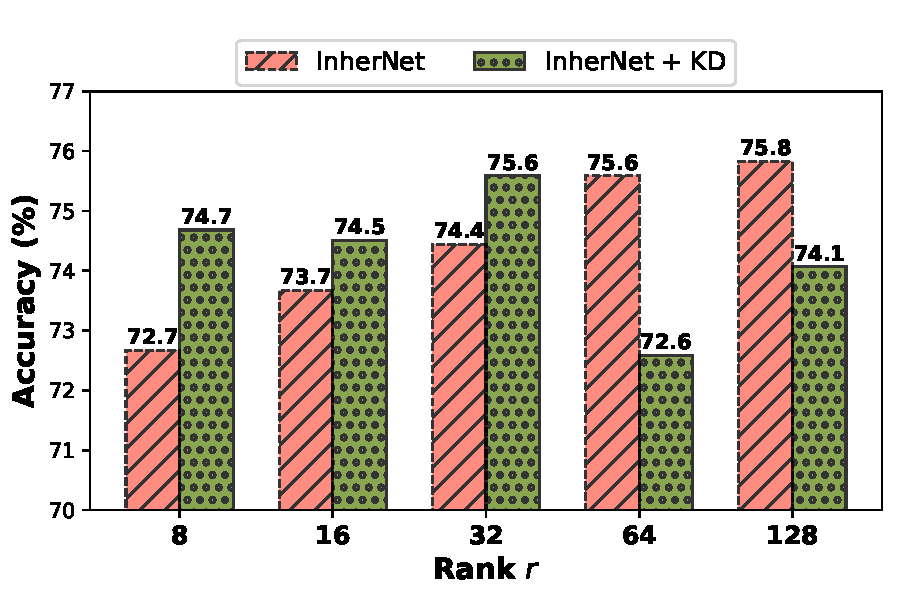
\includegraphics[width=0.6\linewidth]{figures/inhernet_kd_.pdf}
    \vspace{-0.4cm}
    \textbf{\caption{\small The impact of distillation on InherNet of different scales with varying ranks.}
    \label{fig:inhernet_kd}}
    % \vspace{-0.5cm}
\end{figure}

We construct InherNets of different scales based on various ranks ($r = 8, 16, 32, 64, 128$), using them as student networks, and adopt ResNet-56 as the teacher network for knowledge distillation~\citep{hinton2015distilling}. Figure~\ref{fig:inhernet_kd} shows the performance changes of InherNets of different scales before and after distillation. The results indicate that small-scale InherNets ($r \leq 32$) benefit significantly from distillation, with smaller models showing greater improvement. In contrast, large-scale InherNets experience a performance drop after distillation. We speculate that this is because large-scale InherNets already inherit most of the teacher's knowledge and may even outperform the teacher through independent training, InherNet\textsubscript{\ Large} consistently outperforms the teacher network). Therefore, further distillation offers little benefit to such networks and may even have a negative effect.


\begin{figure}[t]
%     % \vspace{-0.1cm}
\centering
    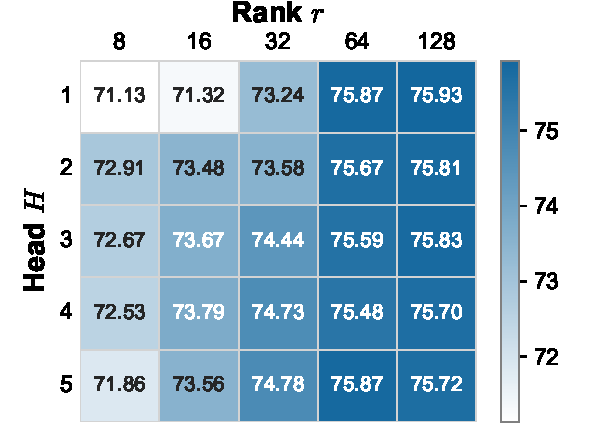
\includegraphics[width=0.5\linewidth]{figures/rank_head.pdf}
    \vspace{-0.4cm}
    \textbf{\caption{\small The impact of rank size $r$ and the number of expert heads $H$ on the performance of the  proposed InherNet.}
    \label{fig:rank_head}}
    % \vspace{-0.5cm}
\end{figure}


\begin{githubquote}
\textbf{Insight 2. Rank significantly affects model performance; using multiple expert heads performs better than a single head.}
\end{githubquote}

We investigate the impact of rank size $r$ and the number of expert heads $H$ on the performance of InherNet. As shown in Figure~\ref{fig:rank_head}, rank exerts a more significant influence on InherNet. We attribute this to the fact that rank directly determines how well InherNet inherits core knowledge from the teacher network, which is crucial for subsequent learning—an advantage that cannot be compensated by simply increasing model parameters such as the number of expert heads. Moreover, we also observe that single-head structures perform worse than multi-head ones. However, increasing the number of heads beyond one ($H > 1$) does not necessarily lead to further gains. We speculate that while multi-head mechanisms combined with gating improve generalization and diversity, too many expert heads may cause overfitting.


\begin{figure*}
    \centering
    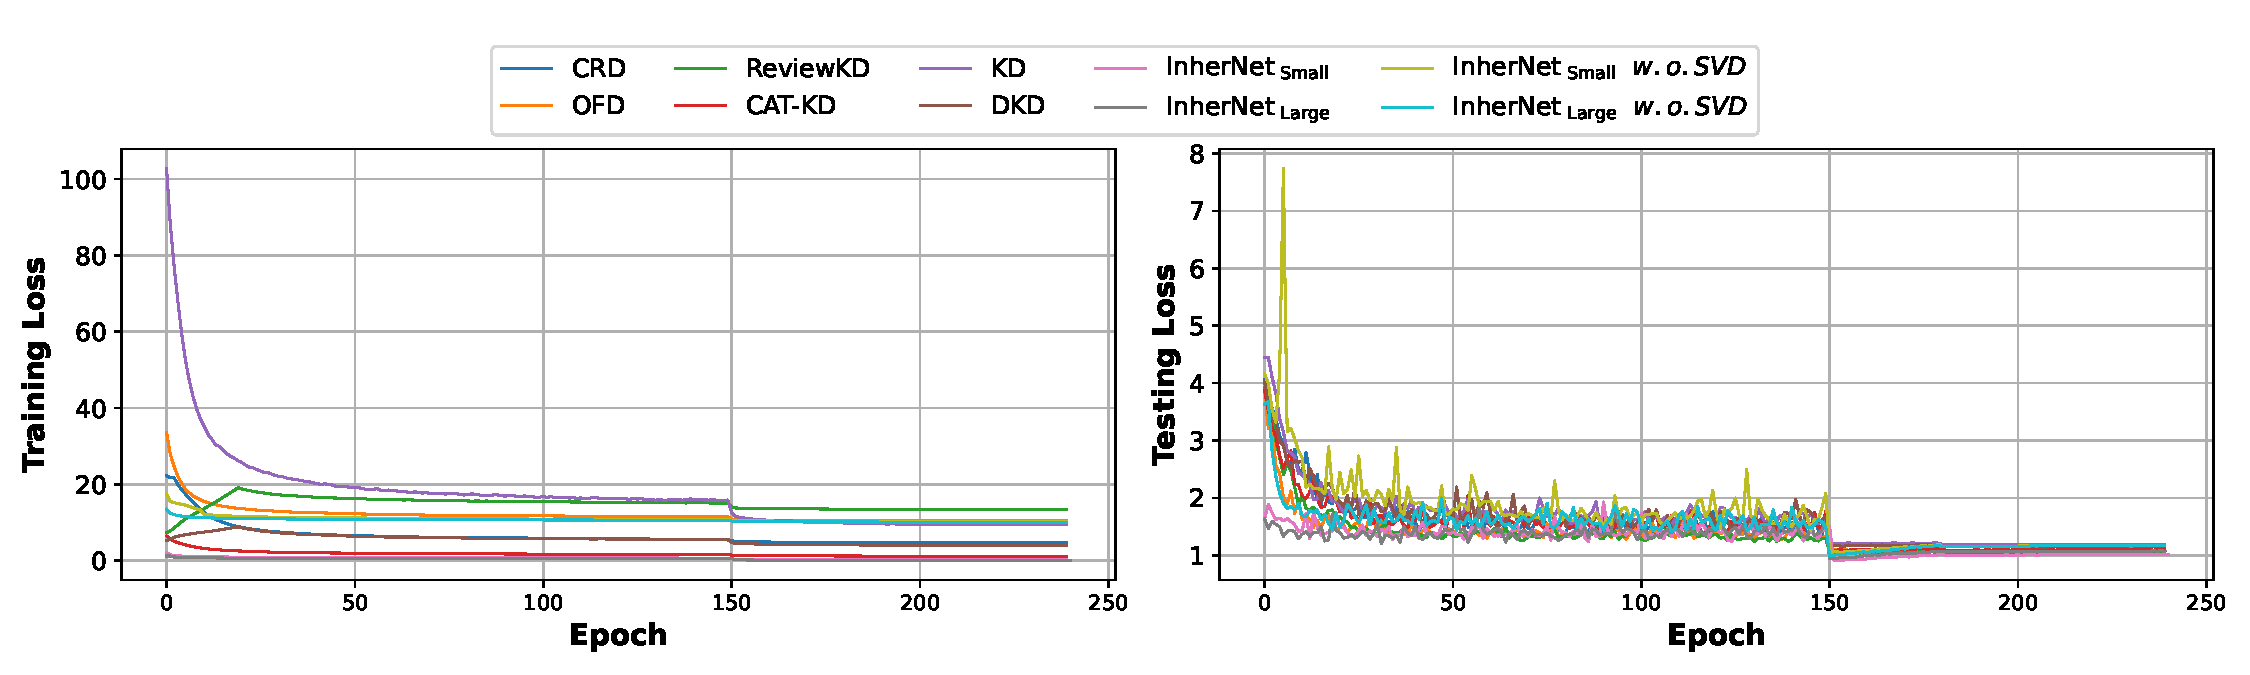
\includegraphics[width=0.9\linewidth]{figures/loss.pdf}
    \vspace{-0.4cm}
    \textbf{\caption{The training and testing loss curves of InherNet and various KD methods during training.}
    \label{fig:loss}}
    % \vspace{-0.5cm}
\end{figure*}

\begin{githubquote}
\textbf{Insight 3. Compared to traditional distillation methods, InherNet converges significantly faster.}
\end{githubquote}

We select the commonly used KD method with epoch=240 as the subject for studying model convergence speed. Figure~\ref{fig:loss} shows the change in training and testing loss during the training process for different methods in a single experiment. The results indicate that InherNet converges significantly faster than traditional KD methods. However, InherNet without SVD initialization shows highly unstable generalization performance during training. This phenomenon strongly supports the effectiveness of the proposed extended SVD method in accelerating model convergence.


\section{Related Work}
\label{sec:related_work}

\subsection{Knowledge Distillation}
\label{sec:kd}
Knowledge distillation (KD)~\citep{hinton2015distilling} is an efficient model compression technique that helps a smaller student network learn better during training by transferring the knowledge of a larger teacher network. Traditional knowledge distillation methods typically focus on minimizing the prediction differences between the teacher and student networks, typically using loss functions like KL divergence calculated from the teacher's logit outputs. ecent research has focused on two main directions: logit distillation~\citep{hinton2015distilling, chen2020online, li2020online, li2022curriculum, zhao2022decoupled, jin2023multi, zhang2023blindly, sun2024logit} and feature distillation~\citep{yim2017gift, peng2019correlation, heo2019comprehensive, chen2021distilling, li2021online, chen2022knowledge, lin2022knowledge, guo2023class}. In logit distillation, the goal is to optimize the similarity of the outputs by matching the prediction probabilities of the teacher and the student, while feature distillation focuses on transferring the intermediate feature representation within the model, providing more fine-grained learning information. However, due to the limited capacity of the student network, especially the performance ceiling imposed by the teacher network, the student's performance often struggles to match that of the teacher~\citep{gou2021knowledge, hu2023teacher, xu2024survey}.

\subsection{Low-Rank Decomposition}
\label{sec:lora}
In recent years, low-rank decomposition has become a key focus in model compression, aiming to reduce storage requirements and improve inference efficiency by approximating weight matrices through the product of low-rank matrices. Initially applied to the weight matrices in convolutional neural networks (CNNs), particularly the 4D tensors of convolutional kernels, early studies~\citep{denton2014exploiting, lebedev2014speeding, tai2015convolutional, xu2019trained, yang2020learning} focused on effective matrix and tensor decomposition methods, such as using CP decomposition to decompose convolutional kernels into multiple low-rank layers~\citep{lebedev2014speeding}. While this approach reduces model complexity, it can lead to issues like vanishing or exploding gradients when scaling to large, deep networks, making training and fine-tuning more challenging~\citep{tai2015convolutional}. To address this, subsequent research has reshaped high-dimensional tensors into 2D matrices and applied techniques like singular value decomposition (SVD) for compression, effectively reducing computational load. For example, channel decomposition~\citep{zhang2015accelerating} using SVD reduces convolution layers to two, with one layer being a $1\times 1$ convolution, and further eliminates small singular value channels to reduce computation. However, these low-rank decomposition methods are typically applicable to specific CNN structures and vision tasks~\citep{wang2026unified}. Moreover, existing methods have not explored the potential link with student networks in KD, while our proposed InherNet aims to establish an effective bridge between the two.

\paragraph{Low-precision low-rank compression.}
Recent work has explored randomized low-precision low-rank factorization for compressing individual matrices and large language models. \cite{saha2023matrix} propose LPLR, a general matrix-compression algorithm that approximates a single matrix $A$ as $A \approx LR$ using randomized sketching and joint low-rank and low-precision factors, with approximation-error guarantees. \cite{saha2024compressing} builds on this idea and applies low-rank and low-precision decompositions to all weight matrices in an LLM, yielding a post-training compression scheme that focuses on bit- and rank-efficient storage while keeping the network architecture unchanged. 

In contrast, our work is not a generic matrix-compression routine but an SVD-driven network inheritance framework: we reparameterize the teacher model into a low-rank, gated one-down-many-ups module and train the resulting InherNet end-to-end. Our analysis centers on inheritance-aware architecture and optimization, including convergence guarantees, parameter-efficiency bounds, and expert specialization, which is theoretically instructive and complementary to \cite{saha2023matrix} and \cite{saha2024compressing}.

\section{The Use of Large Language Models}
\label{sec:LLM}
A Large Language Model (LLM) provided assistance in the preparation of this manuscript. Its role was strictly limited to:

\begin{itemize}
    \item {Proofreading: Checking the text for spelling errors and grammatical accuracy.}
    \item {Improving Clarity: Suggesting alternative phrasing to enhance readability and flow, without changing the scientific meaning.}
\end{itemize}


All changes suggested by the tool were manually reviewed and implemented by the authors to maintain the integrity of the work.



\end{document}
